\begin{table*}[ht]
    \footnotesize
    \setlength{\tabcolsep}{0.9mm}
    \centering

  \caption{
Classification results on three variants of the ScanObjectNN~\cite{uy2019revisiting} dataset and the ModelNet40~\cite{wu20153d} dataset, including the number of trainable parameters and overall accuracy (OA). All methods apply default data augmentation as used in~\cite{zhou2024dynamic}. \textcolor{red}{$^*$} indicates reproduced results. For ScanObjectNN~\cite{uy2019revisiting}, results are reported without voting. For ModelNet40~\cite{wu20153d}, results are shown without and with voting, respectively denoted as (-/-).
}
  \vspace{-10pt}
    \begin{tabular}{lcccccccc}
    
    \toprule
    \multirow{2.3}{*}{Method} &\multirow{2.3}{*}{Reference} &\multirow{2.3}{*}{Tunable params. (M)} &\multirow{2.3}{*}{FLOPs (G)} &\multicolumn{3}{c}{ScanObjectNN} &\multicolumn{2}{c}{ModelNet40}\\
		\cmidrule(r){5-7} \cmidrule{8-9}
	& & & &OBJ\_BG & OBJ\_ONLY &PB\_T50\_RS & Points Num. & OA (\%)      \\
    \midrule
    \multicolumn{9}{c}{\textit{Supervised Learning Only}} \\
    \midrule
    PointNet~\cite{qi2017pointnet} & CVPR 17 & 3.5 & 0.5  & 73.3  & 79.2  & 68.0 & 1k & - / 89.2 \\
    PointNet++~\cite{qi2017pointnet++}   & NeurIPS 17 & 1.5 & 1.7 & 82.3  & 84.3  & 77.9 & 1k & - / 90.7\\
    DGCNN~\cite{wang2019dynamic}  & TOG 19 & 1.8 & 2.4 & 82.8  & 86.2  & 78.1 & 1k & - / 92.9 \\
    MVTN~\cite{hamdi2021mvtn}  & ICCV 21 & 11.2 & 43.7 & -     & -     & 82.8 & 1k & - / 93.8\\
    PointNeXt~\cite{qian2022pointnext} & NeurIPS 22  & 1.4 & 1.6 & -     & -  & 87.7 & 1k & - / 94.0\\
    PointMLP~\cite{ma2022rethinking}  & ICLR 22 &  13.2 & 31.4  & -    & -     & 85.4  & 1k & - / 94.5\\
    RepSurf-U~\cite{ran2022surface} & CVPR 22 & 1.5   & 0.8 &  -  & -    & 84.3  & 1k  & - / 94.4 \\
    ADS~\cite{hong2023attention} & ICCV 23 & -  & -  &  - & -   & 87.5 & 1k  & - / 95.1 \\
    \midrule
    \multicolumn{9}{c}{\textit{ Self-Supervised Representation Learning (Full fine-tuning)}} \\
    \midrule
    % Transformer~\cite{} &  & 22.1 & & 79.86 & 80.55 &  77.24 & 1k & 91.4 \\
    OcCo~\cite{wang2021unsupervised} & ICCV 21 & 22.1 & 4.8 & 84.85 & 85.54 & 78.79 & 1k & - / 92.1 \\
    Point-BERT~\cite{yu2022point}  & CVPR 22 & 22.1 & 4.8  & 87.43 & 88.12 &  83.07 & 1k & - / 93.2 \\
    MaskPoint~\cite{liu2022masked} & ECCV 22 & 22.1 & - & 89.70 & 89.30 &  84.60 & 1k & - / 93.8 \\
    Point-MAE~\cite{pang2022masked}  & ECCV 22 & 22.1 & 4.8 & 90.02 & 88.29 & 85.18 & 1k & - / 93.8 \\
    Point-M2AE~\cite{zhang2022point}  & NeurIPS 22 & 15.3 & 3.6 & 91.22 & 88.81 & 86.43 
 & 1k & - / 94.0\\
    ACT~\cite{dong2022autoencoders} & ICLR 23 & 22.1 & 4.8 & 93.29 & 91.91  & 88.21 & 1k & - / 93.7\\
    \recon~\cite{qi2023contrast} & ICML 23& 43.6 & 5.3 & 94.15 & 93.12  & 89.73 & 1k & - / 93.9  \\
    
    \midrule
    \multicolumn{9}{c}{\textit{Self-Supervised Representation Learning (Efficient fine-tuning)}} \\
    
    \midrule
    Point-BERT~\cite{yu2022point} (baseline)  & CVPR 22 & 22.1 (100\%) & 4.8 & 87.43 & 88.12 & 83.07& 1k & {92.7} / {\color{gray}{93.2}}\\
    + IDPT~\cite{zha2023instance}& ICCV 23 & 1.7 (7.69\%) & 7.2 & {88.12}\dplus{+0.69} & {88.30}\dplus{+0.18} & {83.69}\dplus{+0.62} &1k & {92.6}{\dtplus{-0.1}} / {\color{gray}{{93.4}}}{\color{gray}{\ddplus{+0.2}}} \\
    + DAPT~\cite{zhou2024dynamic}& CVPR 24 & 1.1 (4.97\%) & 5.0 & {91.05}\dplus{+3.62} & {89.67}\dplus{+1.55} & {85.43}\dplus{+2.36} &1k & {93.1}{\dplus{+0.4}} / {\color{gray}{{93.6}}}{\color{gray}{\ddplus{+0.4}}} \\
    + PointGST~\cite{liang2024parameter}& Arxiv 24 & \textbf{0.6} (\textbf{2.71}\%) & 5.0 & {91.39}\dplus{+3.96} & {89.67}\dplus{+1.55} & {85.64}\dplus{+2.57} &1k & {93.4}{\dplus{+0.7}} / {\color{gray}{{93.8}}}{\color{gray}{\ddplus{+0.6}}} \\
    + LST~\cite{sung2022lst}& NeurIPS 22 & 0.8 (3.38\%) & - & {89.15}\dplus{+2.72} & {89.50}\dplus{+1.38} & {83.17}\dplus{+0.10} &1k & {92.9}{\dplus{+0.2}} / {\color{gray}{{93.3}}}{\color{gray}{\ddplus{+0.1}}} \\
    \rowcolor{linecolor!40}+ PLT ({ours})& - & \textbf{0.6} (\textbf{2.71}\%) & 5.0 & {91.57}\dplus{+4.14} & {89.85}\dplus{+1.73} & {86.09}\dplus{+3.02} &1k & {93.5}{\dplus{+0.8}} / {\color{gray}{{94.2}}}{\color{gray}{\ddplus{+1.0}}} \\
    \midrule
    Point-MAE~\cite{pang2022masked} (baseline)& ECCV 22 & 22.1 (100\%)& 4.8& 90.02 & 88.29 & {85.18} & 1k & 93.2 / {\color{gray}{93.8}}\\
    + IDPT~\cite{zha2023instance}& ICCV 23 & 1.7 (7.69\%) & 7.2 & {91.22}\dplus{+1.20} & {90.02}\dplus{+1.73} & {84.94}\dtplus{-0.24} &1k & {93.3}{\dplus{+0.1}} / {\color{gray}{{94.4}}}{\color{gray}{\ddplus{+0.6}}} \\
    + Point-PEFT\textcolor{red}{$^*$}~\cite{tang2024point}& AAAI 24 & 0.7 (3.13\%) & - & {90.19}\dplus{+0.17} & {89.50}\dplus{+1.21} & {84.35}\dtplus{-0.83} &1k & {94.2}{\dplus{+1.0}} / ~~-~~~~~~~~~~~~\\
   + DAPT~\cite{zhou2024dynamic}& CVPR 24 & 1.1 (4.97\%) & 5.0 & {90.88}\dplus{+0.86} & {90.19}\dplus{+1.90} & {85.08}\dtplus{-0.10} &1k & {93.5}{\dplus{+0.3}} / {\color{gray}{{94.0}}}{\color{gray}{\ddplus{+0.2}}} \\
    + PPT\textcolor{red}{$^*$}~\cite{zhang2024positional}& Arxiv 24 & 1.1 (4.97\%) & 5.0 & {89.50}\dtplus{-0.52} & {89.50}\dplus{+1.21} & {84.91}\dtplus{-0.27} &1k & {93.7}{\dplus{+0.5}} / ~~-~~~~~~~~~~~ \\
    + PointGST\cite{liang2024parameter}& Arxiv 24 & \textbf{0.6} (\textbf{2.71}\%) & 5.0 & {91.74}\dplus{+1.72} & {90.19}\dplus{+1.90} & {85.29}\dplus{+0.11} &1k & {93.5}{\dplus{+0.3}} / {\color{gray}{{94.0}}}{\color{gray}{\ddplus{+0.2}}} \\
    + LST~\cite{sung2022lst}& NeurIPS 22 & 0.8 (3.38\%) & 5.0 & {89.67}\dtplus{-0.35} & {89.67}\dplus{+1.38} & {82.75}\dtplus{-2.43} &1k & {93.2}{\ddplus{+0.0}} / {\color{gray}{{93.8}}}{\color{gray}{\ddplus{+0.0}}} \\
    \rowcolor{linecolor!40}+ PLT ({ours})& - & \textbf{0.6} (\textbf{2.71}\%) & 5.0 & {90.88}\dplus{+0.86} & {90.02}\dplus{+1.73} & {85.46}\dplus{+0.28} &1k & {93.8}{\dplus{+0.6}} / {\color{gray}{{94.0}}}{\color{gray}{\ddplus{+0.2}}} \\
    \bottomrule
    \end{tabular}%
  
      \label{tab:sota}

\end{table*}%


\section{Experiments}
\label{sec:experiments}
In this section, we conduct an extensive evaluation of the proposed Point Ladder Tuning (PLT) method across multiple point cloud datasets and tasks. Our experiments aim to validate the effectiveness of PLT in achieving high performance while maintaining parameter efficiency, comparing it against state-of-the-art methods to highlight its advantages.
\subsection{Experimental Settings}
To ensure a fair comparison, we adopted the same experimental setup as used in previous fine-tuning methods~\cite{zha2023instance, zhou2024dynamic} for each baseline. During training, the weights of the pre-trained model were frozen, and only a limited number of parameters in the added modules were fine-tuned. All experiments were performed on a single GeForce RTX 3090 GPU.

\subsection{3D Object Classification}
\label{sec:classification}
\textbf{Object Classification on Real-World Dataset.} While most pre-trained point cloud models are trained on synthetic datasets like ShapeNet~\cite{chang2015shapenet}, which consist of clean, uniformly distributed point clouds, real-world point clouds often present additional challenges such as noise, missing data, and diverse distributions. To evaluate performance in these more realistic scenarios, we use the ScanObjectNN dataset~\cite{uy2019revisiting}, which comprises approximately 15k point cloud samples across 15 categories captured in indoor scenes, often containing background interference and occlusions. As shown in Tab.~\ref{tab:sota}, we evaluate PLT on three variants of the ScanObjectNN dataset (OBJ\_BG, OBJ\_ONLY, and PB\_T50\_RS), using PointBERT~\cite{yu2022point} and PointMAE~\cite{pang2022masked} as baselines.

Our PLT method demonstrates notable accuracy improvements over full fine-tuning in all settings, using only 2.71\% of the parameters. Specifically, PLT achieves gains of 4.14\%, 1.73\%, and 3.02\% on the three ScanObjectNN variants with PointBERT. Compared to the state-of-the-art model, PointGST, PLT achieves accuracy improvements of 0.45\% on PointBERT and 0.17\% on PointMAE under the most challenging PB\_T50\_RS setting in ScanObjectNN, showcasing the robustness and efficiency of our approach in handling real-world point cloud data.


%\textbf{Object Classification on Real-World Dataset.} Pre-trained Point cloud models are typically trained on the ShapeNet dataset~\cite{chang2015shapenet}, which consists of clean, uniformly distributed point clouds. However, real-world point clouds often suffer from issues such as noise and missing point, leading to diverse and challenging distributions. To evaluate the performance in these more realistic conditions, we use the ScanObjectNN dataset~\cite{uy2019revisiting}, which contains approximately 15k point cloud samples across 15 categories. These point clouds are captured in indoor scenes and often include background interference and occlusions from other objects. As shown in Tab.\ref{tab:sota} We conduct experiments on on three variants of the ScanObjectNN dataset~\cite{uy2019revisiting} (OBJ\_BG, OBJ\_ONLY, and PB\_T50\_RS), using two baseline models, PointBERT~\cite{yu2022point} and PointMAE~\cite{pang2022masked}, to assess the effectiveness of our PLT. 

%Notably, PLT achieved better accuracy than full fine-tuning across all settings while utilizing only 2.71\% of the parameters. Especially, PLT achieved increases of 4.14\%, 1.73\%, and 3.02\% in the three ScanObjectNN~\cite{uy2019revisiting} variants on Point-BERT. Compared to the state-of-the-art model PointGST, our LST improved accuracy by 0.45\% on PointBERT~\cite{yu2022point} and 0.17\% on PointMAE~\cite{pang2022masked} under the most challenging setting, PB\_T50\_RS, in ScanObjectNN~\cite{uy2019revisiting}.

%\textbf{Object Classification on Synthetic Dataset.} We also conduct experiments on the ModelNet dataset~\cite{wu20153d}, which includes 12,311 clean 3D CAD models across 40 categories. Following DAPT~\cite{zhou2024dynamic}, we split the ModelNet40 dataset into 9,843 training samples and 2,468 testing samples. During training, we applied standard data augmentation techniques, including random scaling and random translation. As shown in Tab.\ref{tab:sota}, without voting, our PLT achieved accuracy rates of 93.8\% and 93.5\% on PointMAE and PointBERT, respectively, which were 0.6\% and 0.8\% higher than full fine-tuning.. With voting, PLT continues to outperform full fine-tuning, especially on PointBERT, with an accuracy increase of 1.0\%.

%\textbf{Few-shot Learning.}We further conduct experiments on ModelNet40 to evaluate its transfer learning ability in few-shot setting. Following prior work~\cite{pang2022masked,zha2023instance,zhou2024dynamic}, we adopt the n-way, n-shot setting. As shown in Tab.~\ref{tab:fewshot}, PLT outperforms fully fine-tuned models and state-of-the-art models like IDPT~\cite{zha2023instance} and DAPT~\cite{zhou2024dynamic} in most cases, demonstrating its effectiveness in few-shot learning.

%\textbf{Compared with Other PETL Methods.}As illustrated in Tab.~\ref{tab:origin_finetuning}, using VPT~\cite{jia2022visual} for fine-tuning in PointMAE~\cite{pang2022masked} leads to a notable performance drop compared to full fine-tuning, particularly with a 4.09\% decrease in the PB\_T5\_RS setting. Similarly, while adapters~\cite{houlsby2019parameter} shows slight improvements on the OBJ\_ONLY task, but significant performance drops in other settings. LST~\cite{sung2022lst} demonstrate substantial gains on OBJ\_ONLY, but underperformed elsewhere. We also compare PEFT methods PEFT methods from various fields on the challenging PB\_T50\_RS variant of ScanObjectNN~\cite{uy2019revisiting}. As shown in the Tab.~\ref{tab:compare}, our methods are more effective than those proposed in NLP, 2D, and 3D areas. 

\textbf{Object Classification on Synthetic Dataset.} We conduct experiments on the ModelNet dataset~\cite{wu20153d}, which contains 12,311 clean 3D CAD models spanning 40 categories. Following the protocol in DAPT~\cite{zhou2024dynamic}, we split ModelNet40 into 9,843 training samples and 2,468 testing samples. Standard data augmentation techniques, including random scaling and random translation, were applied during training. As shown in Tab.~\ref{tab:sota}, without voting, PLT achieves accuracy rates of 93.8\% and 93.5\% on PointMAE and PointBERT, respectively—representing gains of 0.6\% and 0.8\% over full fine-tuning. When using voting, PLT continues to outperform full fine-tuning, notably improving PointBERT’s accuracy by an additional 1.0\%.

\textbf{Few-shot Learning.} We further evaluate PLT’s transfer learning capabilities in a few-shot setting on ModelNet40. Adopting the n-way, n-shot setup used in prior works~\cite{pang2022masked,zha2023instance,zhou2024dynamic}, we observe that PLT consistently outperforms fully fine-tuned models and state-of-the-art methods such as IDPT~\cite{zha2023instance} and DAPT~\cite{zhou2024dynamic} across most scenarios, demonstrating its efficacy in few-shot learning (see Tab.~\ref{tab:fewshot}).

\textbf{Comparison with Other PETL Methods.} As illustrated in Tab.~\ref{tab:origin_finetuning}, using VPT~\cite{jia2022visual} for fine-tuning in PointMAE~\cite{pang2022masked} results in a marked performance drop compared to full fine-tuning, with a decrease of 4.09\% in the PB\_T50\_RS setting. Similarly, while adapters~\cite{houlsby2019parameter} show modest improvements on the OBJ\_ONLY task, they exhibit significant drops in other scenarios. LST~\cite{sung2022lst} provides substantial gains on OBJ\_ONLY but underperforms in other settings. We further compare various PEFT methods across challenging PETL scenarios, including the PB\_T50\_RS variant of ScanObjectNN~\cite{uy2019revisiting}. As shown in Tab.~\ref{tab:compare}, our PLT method demonstrates superior effectiveness across NLP, 2D, and 3D applications.

\begin{table}[!t]
  \centering
  \scriptsize
    \setlength{\tabcolsep}{0.7mm}
  \caption{Few-shot learning on ModelNet40\cite{wu20153d}. Overall accuracy (\%)$\pm$the standard deviation (\%) without voting is reported.}
    \begin{tabular}{lccccc}
    \toprule
   \multirow{2.3}{*}{Methods}&\multirow{2.3}{*}{Reference} & \multicolumn{2}{c}{5-way} & \multicolumn{2}{c}{10-way} \\
\cmidrule{3-6}  &        & 10-shot & 20-shot & 10-shot & 20-shot \\
    % \midrule
    % \multicolumn{6}{c}{\textit{with Self-Supervised Representation Learning (Full fine-tuning)}} \\
    % \midrule
    % % OcCo~\cite{wang2021unsupervised} & ICCV 21      & 94.0$\pm$3.6& 95.9$\pm$2.3 & 89.4$\pm$5.1 & 92.4$\pm$4.6 \\
    % % Point-BERT~\cite{yu2022point}  &  CVPR 22    & 94.6$\pm$3.1 & 96.3$\pm$2.7 & 91.0$\pm$5.4 & 92.7$\pm$5.1 \\
    % MaskPoint~\cite{liu2022masked}  &   ECCV 22   & 95.0$\pm$3.7 & 97.2$\pm$1.7 & 91.4$\pm$4.0 & 93.4$\pm$3.5 \\
    % % Point-MAE~\cite{pang2022masked} &   ECCV 22   & 96.3$\pm$2.5 & 97.8$\pm$1.8 & 92.6$\pm$4.1 & 95.0$\pm$3.0 \\
    % Point-M2AE~\cite{zhang2022point} &  NeurIPS 22    & 96.8$\pm$1.8 & 98.3$\pm$1.4 & 92.3$\pm$4.5 & 95.0$\pm$3.0 \\
    % % ACT~\cite{dong2022autoencoders}  & ICLR 23      & 96.8$\pm$2.3 & 98.0$\pm$1.4 & 93.3$\pm$4.0 & 95.6$\pm$2.8 \\
    % VPP~\cite{qi2024vpp} &  NeurIPS 23    & 96.9$\pm$1.9 & 98.3$\pm$1.5 & 93.0$\pm$4.0 & 95.4$\pm$3.1 \\
    % I2P-MAE~\cite{zhang2023learning} &  CVPR 23    & 97.0$\pm$1.8 & 98.3$\pm$1.3 & 92.6$\pm$5.0 & 95.5$\pm$3.0 \\
    % \recon~\cite{qi2023contrast}  & ICML 23      & 97.3$\pm$1.9 & 98.9$\pm$1.2 & 93.3$\pm$3.9 & 95.8$\pm$3.0 \\
    % PointMamba~\cite{liang2024pointmamba} &  NeurIPS 24 & 96.9$\pm$2.0 & 99.0$\pm$1.1 & 93.0$\pm$4.4 & 95.6$\pm$3.2 \\
    % \midrule
    % \multicolumn{6}{c}{\textit{with Self-Supervised Representation Learning (Efficient fine-tuning)}} \\
    \midrule
   Point-BERT~\cite{yu2022point} (baseline) & CVPR 22 &94.6$\pm$3.1 & 96.3$\pm$2.7 & 91.0$\pm$5.4 & 92.7$\pm$5.1 \\
   + IDPT~\cite{zha2023instance} & ICCV 23    & 96.0$\pm$\textbf{1.7}& 97.2$\pm$2.6& 91.9$\pm$4.4& 93.6$\pm$3.5\\
   + DAPT~\cite{zhou2024dynamic} & CVPR 24&95.8$\pm$2.1 &97.3$\pm$1.3 &92.2$\pm$4.3 &94.2$\pm$3.4 \\
   + PointGST~\cite{liang2024parameter}  & Arxiv 24&96.5$\pm$2.4 &97.9$\pm$2.0 &92.7$\pm$4.2 &95.0$\pm$\textbf{2.8} \\
   + LST~\cite{sung2022lst}  & NIPS 22&94.3$\pm$2.6 &97.1$\pm$1.8 &90.6$\pm$4.7 &93.7$\pm$3.7 \\
   \rowcolor{linecolor!40}+ PLT (\textbf{ours}) & -&\textbf{96.9}$\pm$2.0 &\textbf{98.8}$\pm$\textbf{1.1}&\textbf{93.3}$\pm$\textbf{4.0} &\textbf{95.5}$\pm$3.1 \\
    \midrule
    Point-MAE~\cite{pang2022masked} (baseline) &ECCV 22 & 96.3$\pm$2.5 & 97.8$\pm$1.8 & 92.6$\pm$4.1 & 95.0$\pm$3.0\\
   + IDPT~\cite{zha2023instance} &   ICCV 23    & 97.3$\pm$2.1& 97.9$\pm$1.1& 92.8$\pm$4.1& 95.4$\pm$\textbf{2.9}\\
   + DAPT~\cite{zhou2024dynamic} & CVPR 24 & 96.8$\pm$\textbf{1.8}  &  98.0$\pm$1.0 & 93.0$\pm$\textbf{3.5} & \textbf{95.5}$\pm$3.2  \\
   % + PointGST~\cite{liang2024parameter} & Arxiv 24 & \textbf{98.0}$\pm$\textbf{1.8}  &  98.3$\pm$\textbf{0.9} & \textbf{93.7}$\pm$\textbf{4.0} & \textbf{95.7}$\pm$\textbf{2.4}  \\
   + LST~\cite{sung2022lst}  & NIPS 22&96.6$\pm$2.5 &97.5$\pm$1.7 &92.0$\pm$4.4 &94.9$\pm$3.2 \\
   \rowcolor{linecolor!40}+ PLT (\textbf{ours}) & - & \textbf{97.2}$\pm$2.2  &  \textbf{98.9}$\pm$\textbf{0.9} & \textbf{93.2}$\pm$4.2 & \textbf{95.5}$\pm$\textbf{2.9}  \\
   \midrule
   ACT~\cite{dong2022autoencoders} (baseline) & ICLR 23 & 96.8$\pm$2.3 & 98.0$\pm$1.4 & 93.3$\pm$4.0 & 95.6$\pm$2.8\\
   + IDPT~\cite{zha2023instance} &   ICCV 23    & 96.8$\pm$1.9& 98.3$\pm$1.2& 92.5$\pm$4.1& 95.3$\pm$3.3\\
   + DAPT~\cite{zhou2024dynamic} & CVPR 24 & 95.3$\pm$2.8  &  97.1$\pm$1.7 & 89.8$\pm$4.8 & 94.1$\pm$3.6  \\
   + PPT~\cite{zhang2024positional}  & Arxiv 24 & \textbf{97.1}$\pm$2.3 &98.1$\pm$1.8 &91.8$\pm$4.3 &94.9$\pm$3.4 \\
   + PointGST~\cite{liang2024parameter} & Arxiv 24 & 97.2$\pm$1.9  &  98.3$\pm$1.3 & 92.9$\pm$4.2 & 95.7$\pm$\textbf{2.6}  \\
   + LST~\cite{sung2022lst}  & NIPS 22&96.2$\pm$2.6 &98.0$\pm$1.9 &92.6$\pm$4.4 &94.9$\pm$3.4 \\
   \rowcolor{linecolor!40}+ PLT (\textbf{ours}) & - & 96.9$\pm$\textbf{1.8}  &  \textbf{98.9}$\pm$\textbf{1.0} & \textbf{93.4}$\pm$\textbf{4.0} & \textbf{95.9}$\pm$3.1  \\
    \bottomrule
    % \vspace{-12pt}
    \end{tabular}%
  \label{tab:fewshot}%
\end{table}%

\begin{table}
\scriptsize
\setlength{\tabcolsep}{1.9mm}
\centering
\caption{Comparisons of parameter efficient transfer learning methods from NLP and 2D Vision on the hardest variant of ScanObjectNN~\cite{uy2019revisiting}. Overall accuracy (\%) without voting is reported. \#TP represents the tunable parameters. \textcolor{red}{$^*$} denotes reproduced results.}
\label{tab:compare}
\begin{tabular}{ lcccc }
\toprule
 Method &Reference& Design for &\#TP (M) & PB\_T50\_RS \\
\midrule
 Point-MAE~\cite{pang2022masked}  &ECCV 22 & - & 22.1 & 85.18  \\
 Linear probing &- & - & 0.3& 75.99\\
 \midrule
  + Adapter~\cite{houlsby2019parameter}&ICML 19 & NLP & 0.9 & 83.93 \\
  + Perfix tuning~\cite{li2021prefix}& ACL 21 & NLP &0.7 & 77.72  \\
  + BitFit~\cite{zaken2022bitfit} & ACL 21 & NLP &0.3 & 82.62    \\
  + LST~\cite{sung2022lst} & NeurIPS 22 & NLP & 0.8 & 82.75\\
  + LoRA~\cite{hu2021lora} & ICLR 22 & NLP & 0.9&  81.74   \\
  % + DEPT~\cite{shi2024dept} & ICLR 24 & NLP & 0.3 & 79.70\\
  + FourierFT~\cite{Gao2024Fourier} & ICML 24 & NLP &0.3 & 78.57\\
  \midrule
  + VPT-Deep~\cite{jia2022visual}&ECCV 22 & 2D &0.4 &  81.09 \\
  + AdaptFormer~\cite{chen2022adaptformer} &NeurIPS 22 & 2D &0.9  & 83.45 \\
  + SSF~\cite{lian2022scaling} & NeurIPS 22 & 2D &0.4  & 82.58\\
  + FacT~\cite{jie2023fact} & AAAI 23 & 2D & 0.5 & 78.76\\
  % + BI-AdaptFormer~\cite{jie2023revisiting} & ICCV 23 & 2D & 0.4 & 83.66\\
  + SCT~\cite{zhao2024sct} & IJCV 24 & 2D & 0.3 & 80.40\\
  \midrule
  + IDPT~\cite{zha2023instance} &ICCV 23 & 3D & 1.7 &84.94\\
  + Point-PEFT\textcolor{red}{$^*$}~\cite{tang2024point} & AAAI 24 & 3D & 0.7 &84.35\\
  + DAPT~\cite{zhou2024dynamic} & CVPR 24 & 3D & 1.1 & 85.08 \\
  + PPT\textcolor{red}{$^*$}~\cite{zhang2024positional} & Arxiv 24 & 3D & 1.1 & 84.91\\
  + PointGST~\cite{liang2024parameter} & Arxiv 24 & 3D & 0.6 & 85.29\\
  % + PointLoRA~\cite{wang2025pointlora} & CVPR 25 & 3D & 0.8 & \textbf{85.53}\\
  \rowcolor{linecolor!40}+ PLT (\textbf{ours}) & - & 3D & 0.6 & \textbf{85.53} \\
\bottomrule
\end{tabular}
\end{table}


\begin{figure}
    \centering
    \begin{subfigure}{0.235\textwidth}
        \centering
        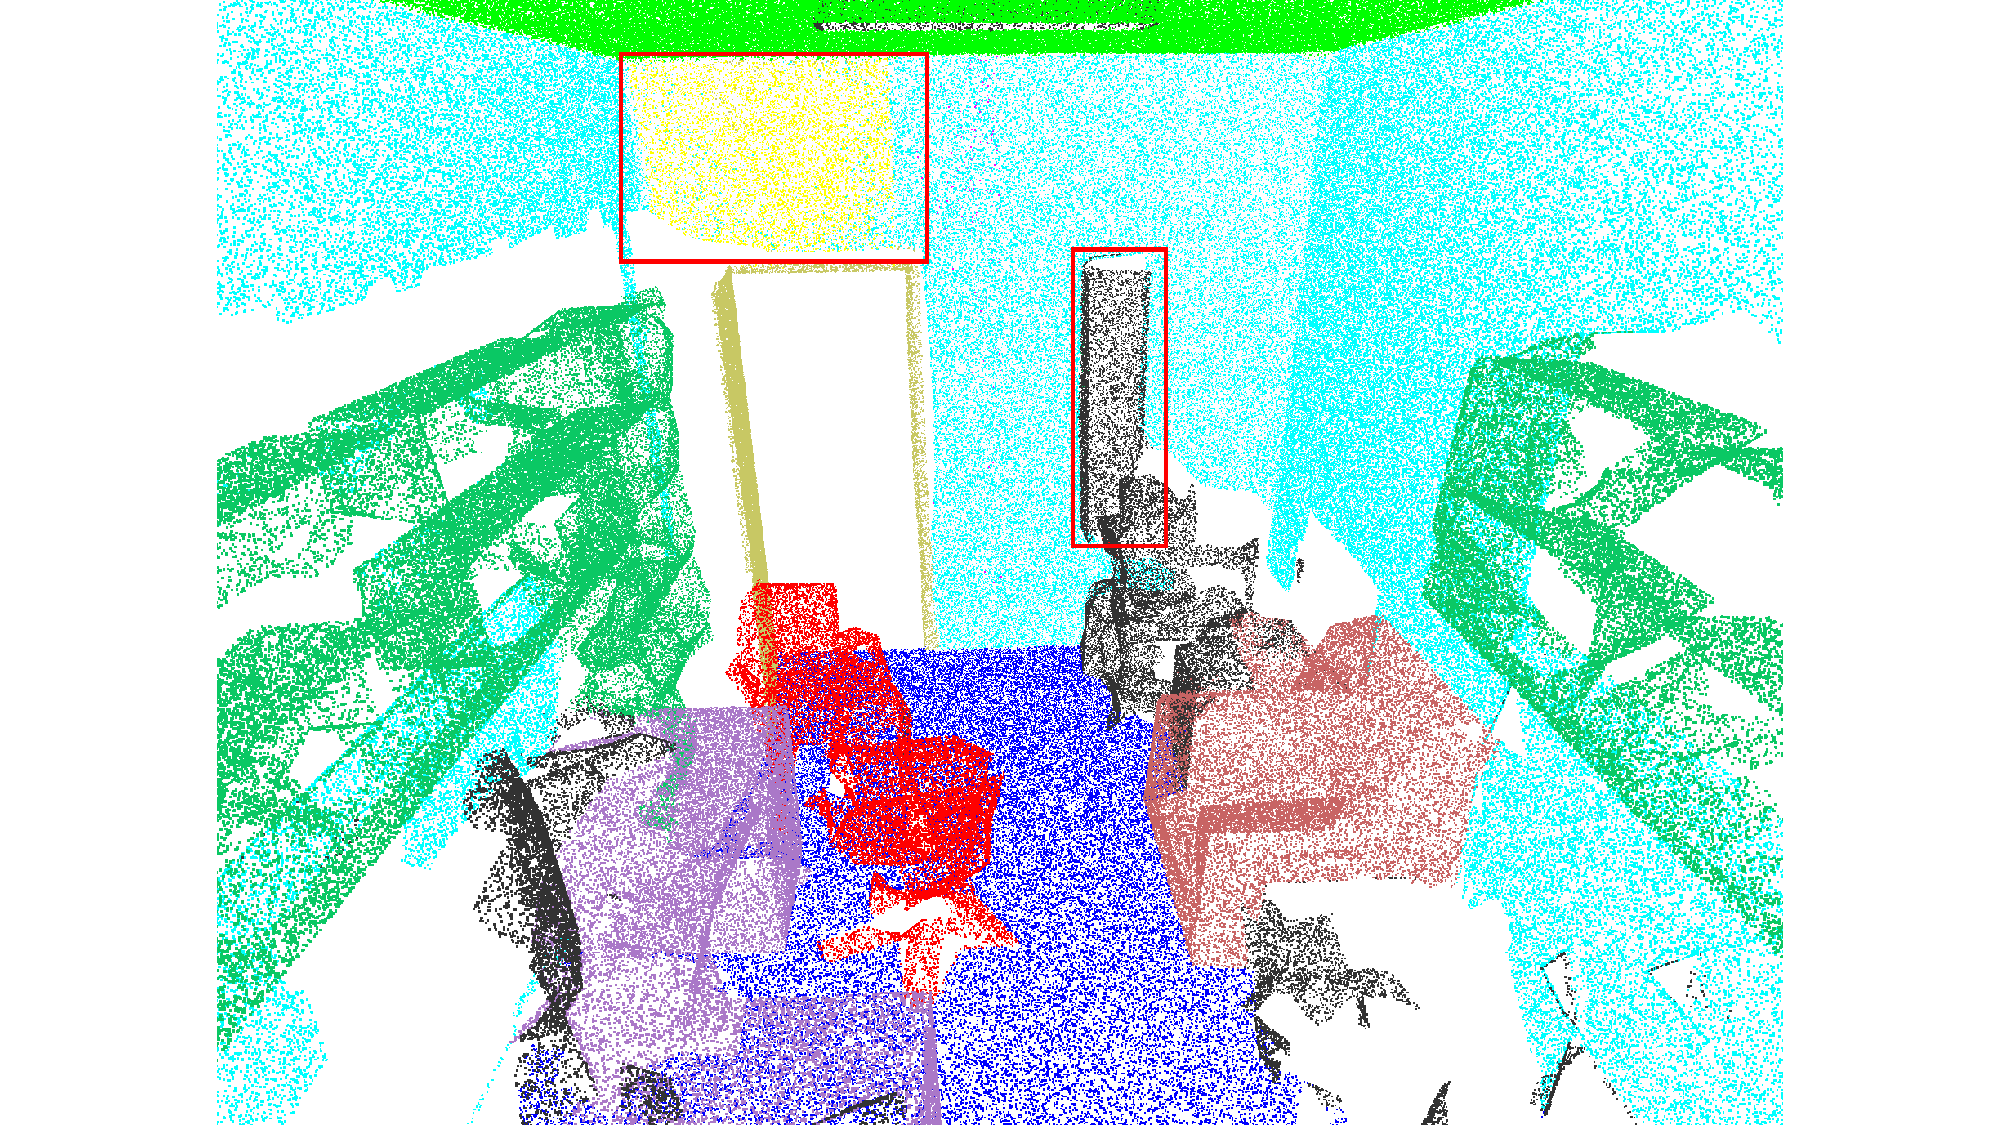
\includegraphics[width=\linewidth]{fig/S3DIS/PointMAE.pdf}
        % \caption*{\textbf{\#TP}:22.1M \textbf{\#OA}:85.18}
        \caption{Full fine-tuning}
        \label{fig:s3dis1}
    \end{subfigure}
    \hfill
    \begin{subfigure}{0.235\textwidth}
        \centering
        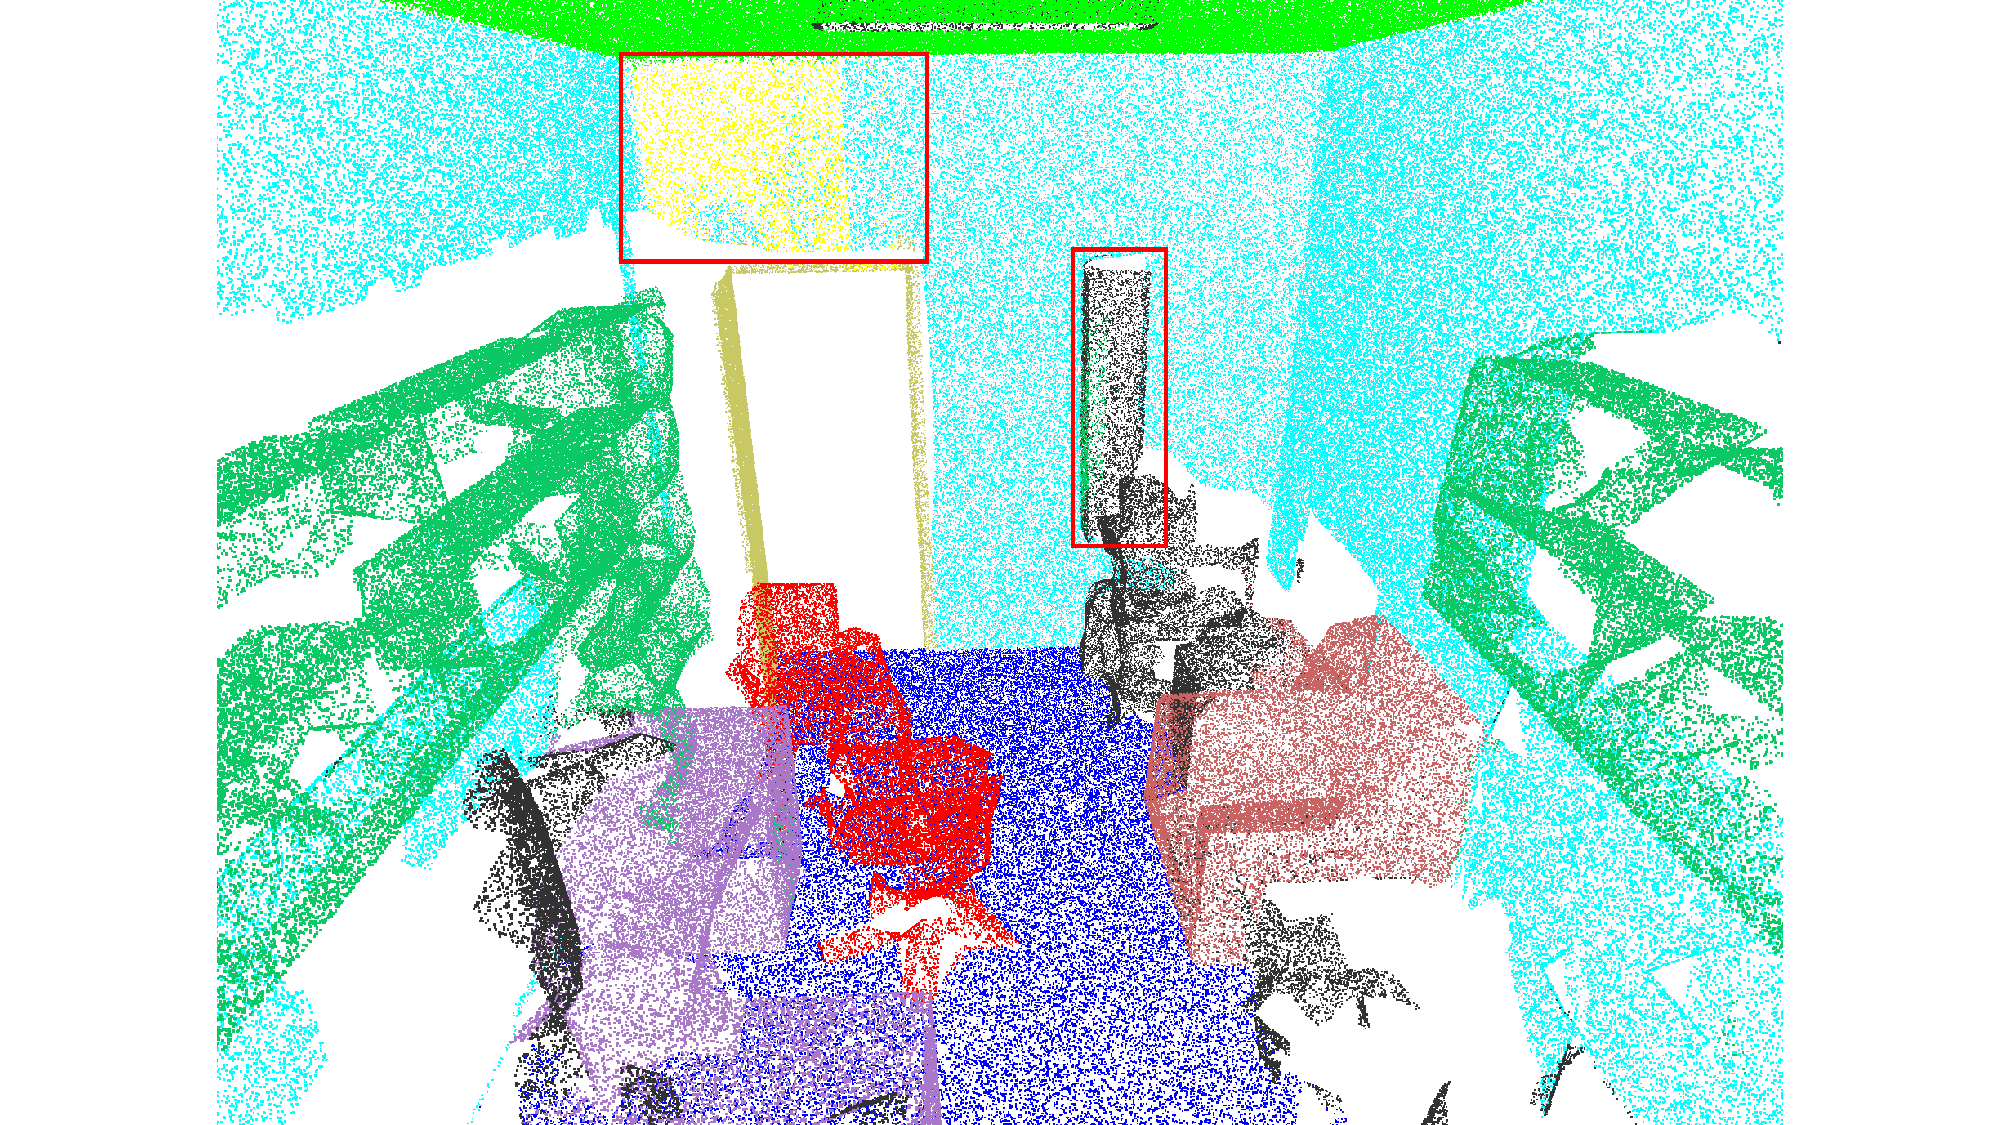
\includegraphics[width=\linewidth]{fig/S3DIS/DAPT.pdf}
        % \caption*{\textbf{\#TP}:1.7M \textbf{\#OA}:84.94}
        \caption{DAPT~\cite{zhou2024dynamic}}
        \label{fig:s3dis2}
    \end{subfigure}
    \hfill
    \begin{subfigure}{0.235\textwidth}
        \centering
        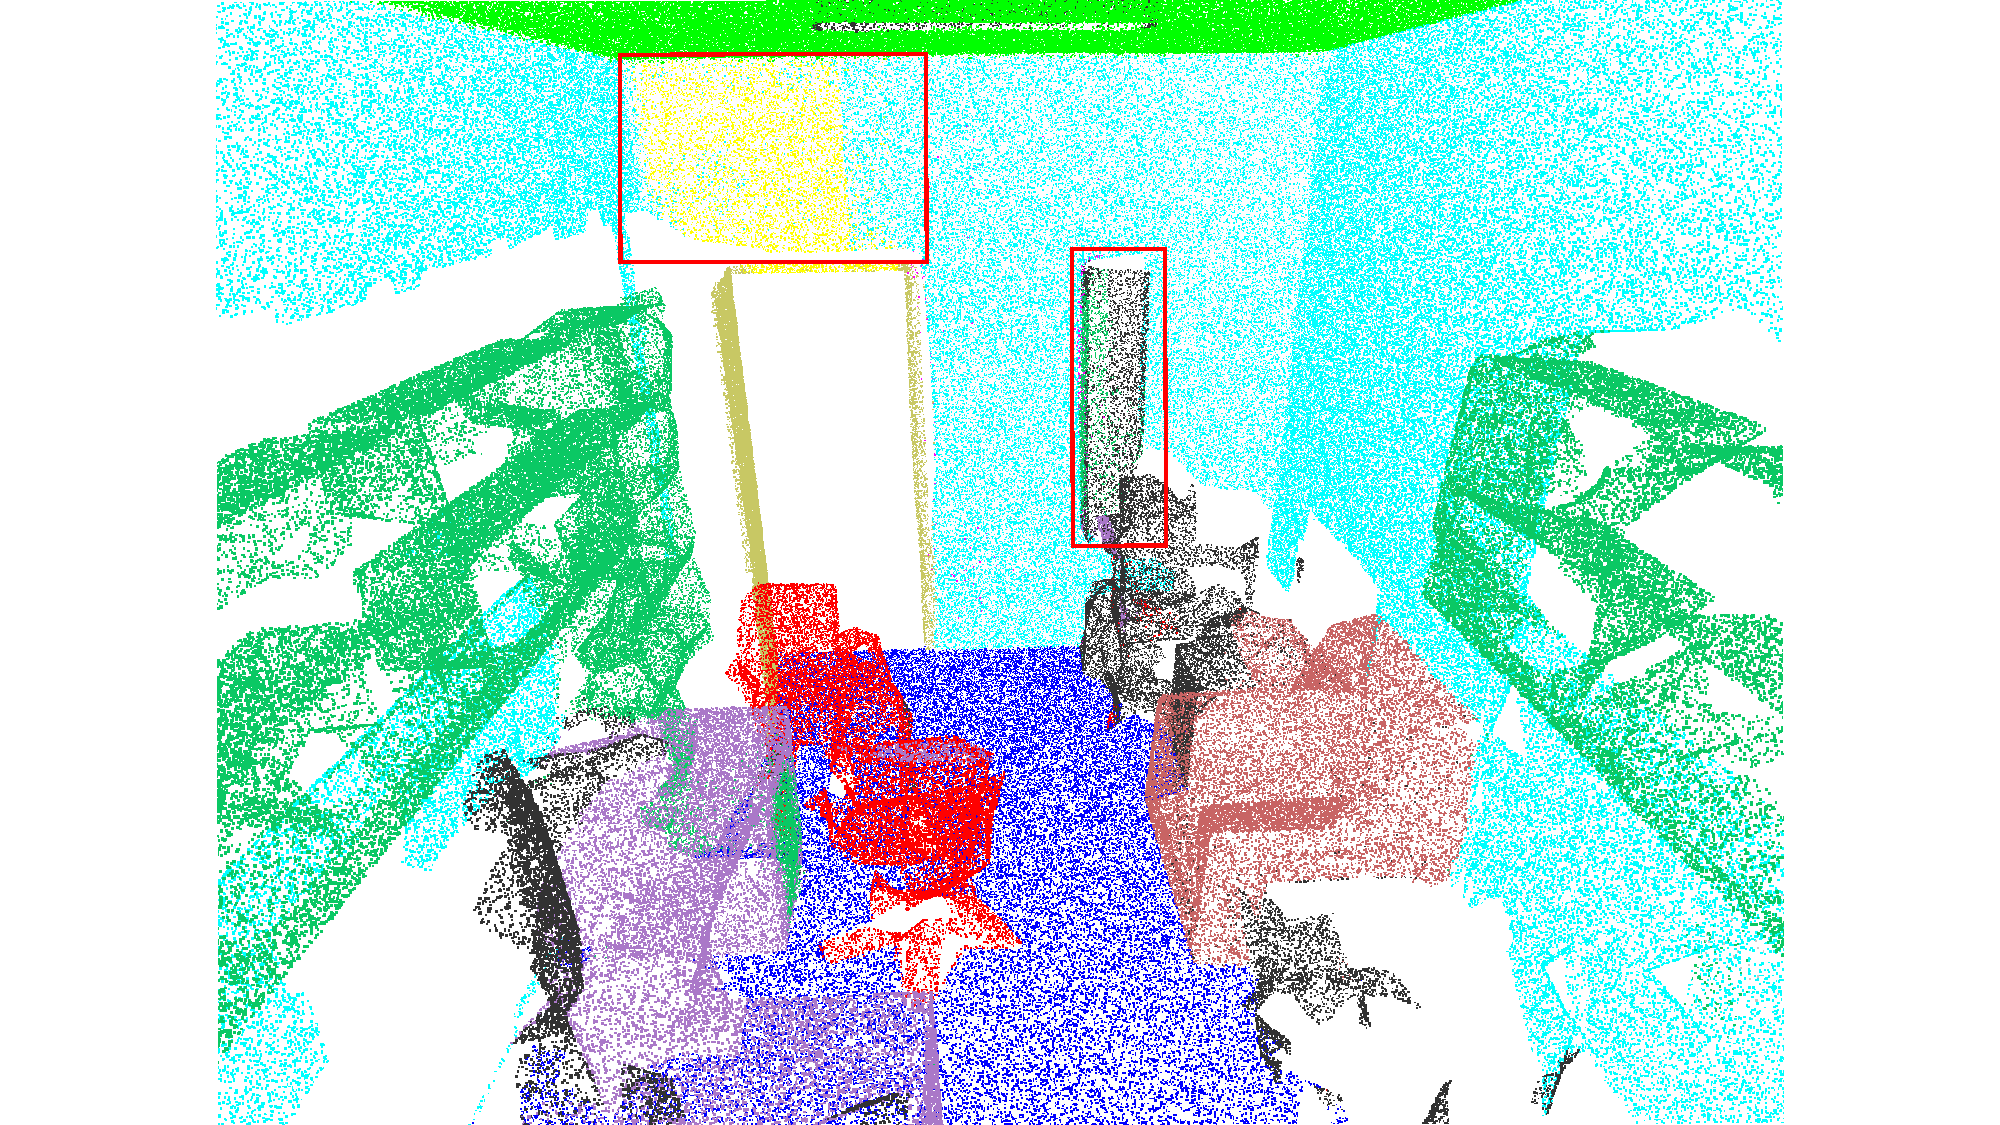
\includegraphics[width=\linewidth]{fig/S3DIS/IDPT.pdf}
        % \caption*{\textbf{\#TP}:1.1M \textbf{\#OA}:85.08}
        \caption{IDPT~\cite{zha2023instance}}
        \label{fig:s3dis3}
    \end{subfigure}
    \hfill
    \begin{subfigure}{0.235\textwidth}
        \centering
        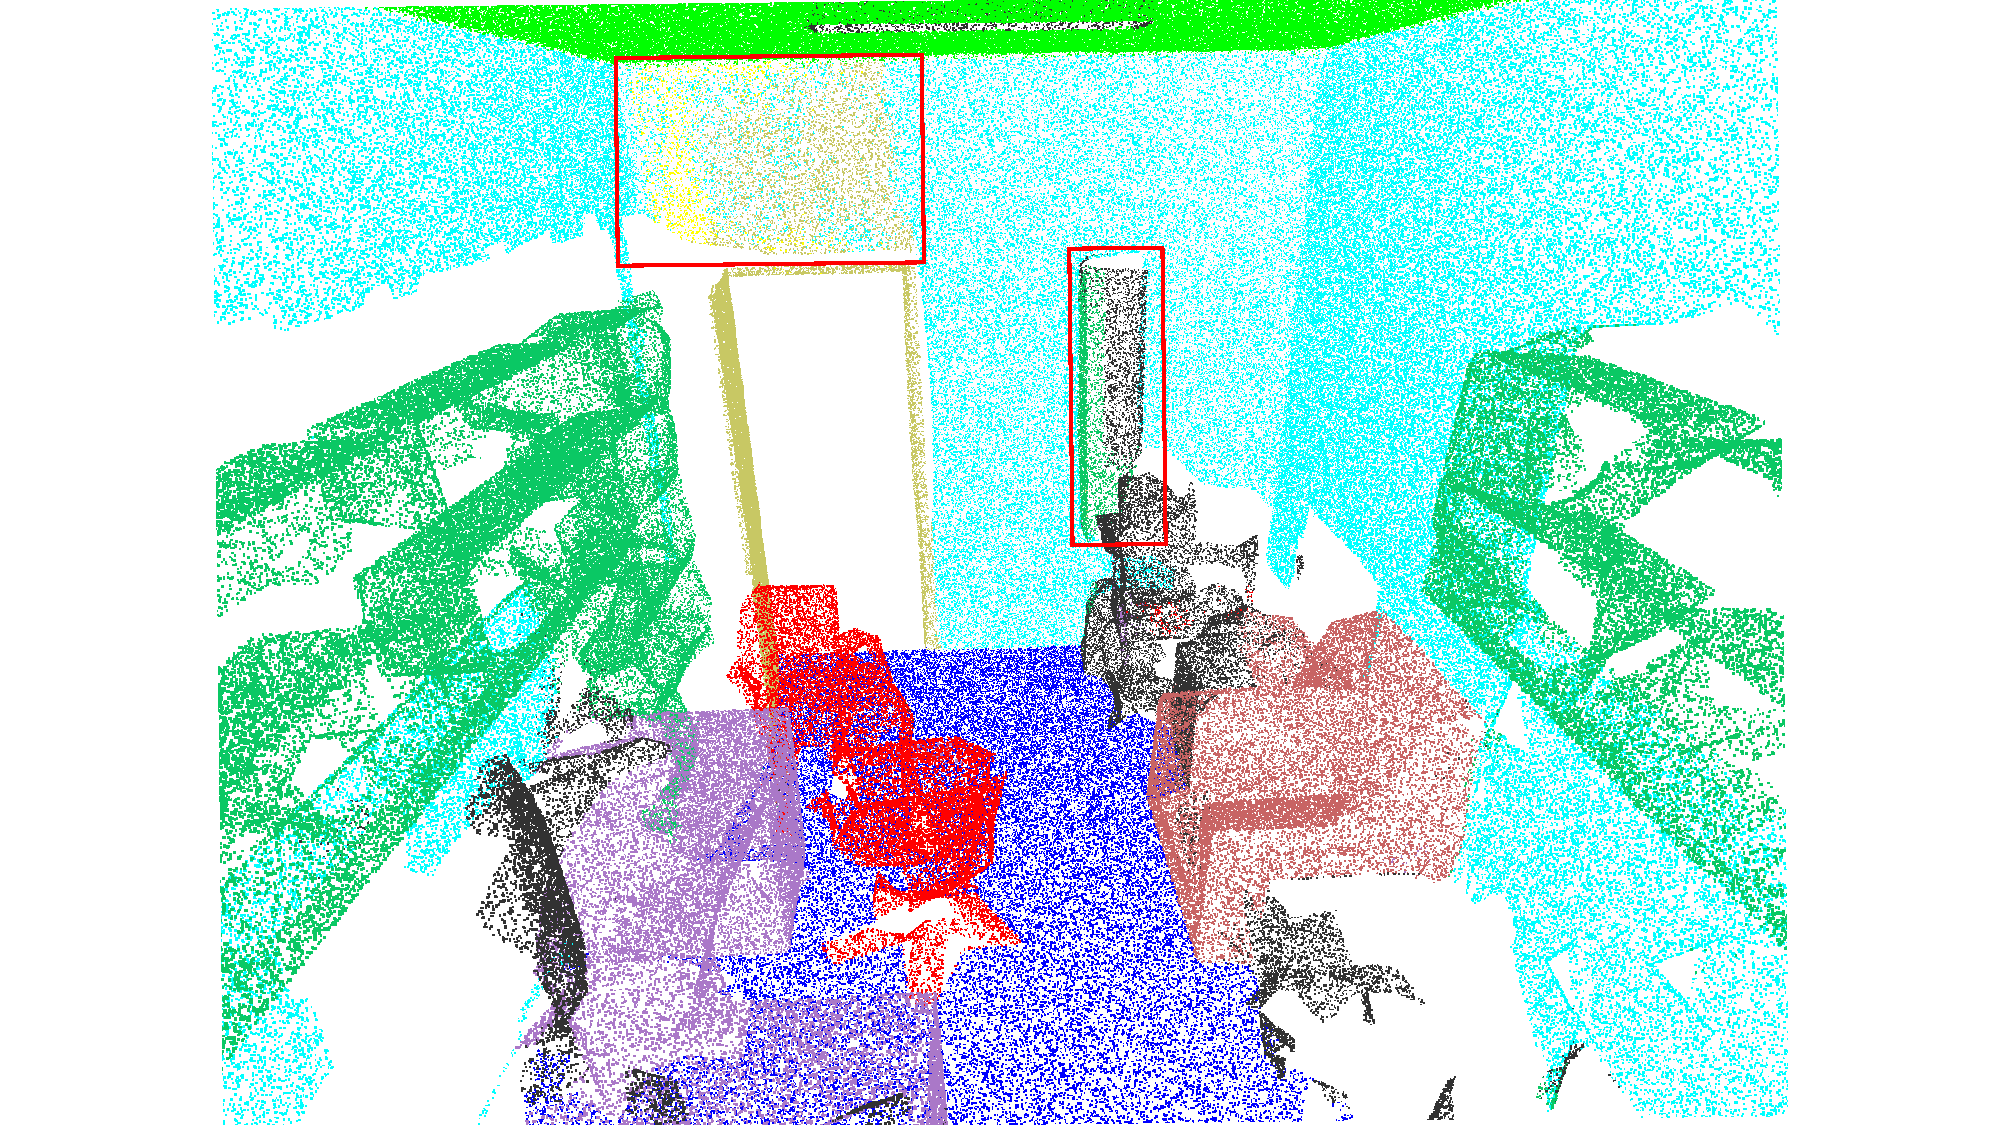
\includegraphics[width=\linewidth]{fig/S3DIS/PPT.pdf}
        % \caption*{\textbf{\#TP}:1.1M \textbf{\#OA}:84.91}
        \caption{PPT~\cite{zhang2024positional}}
        \label{fig:s3dis4}
    \end{subfigure}
    \hfill
    \begin{subfigure}{0.235\textwidth}
        \centering
        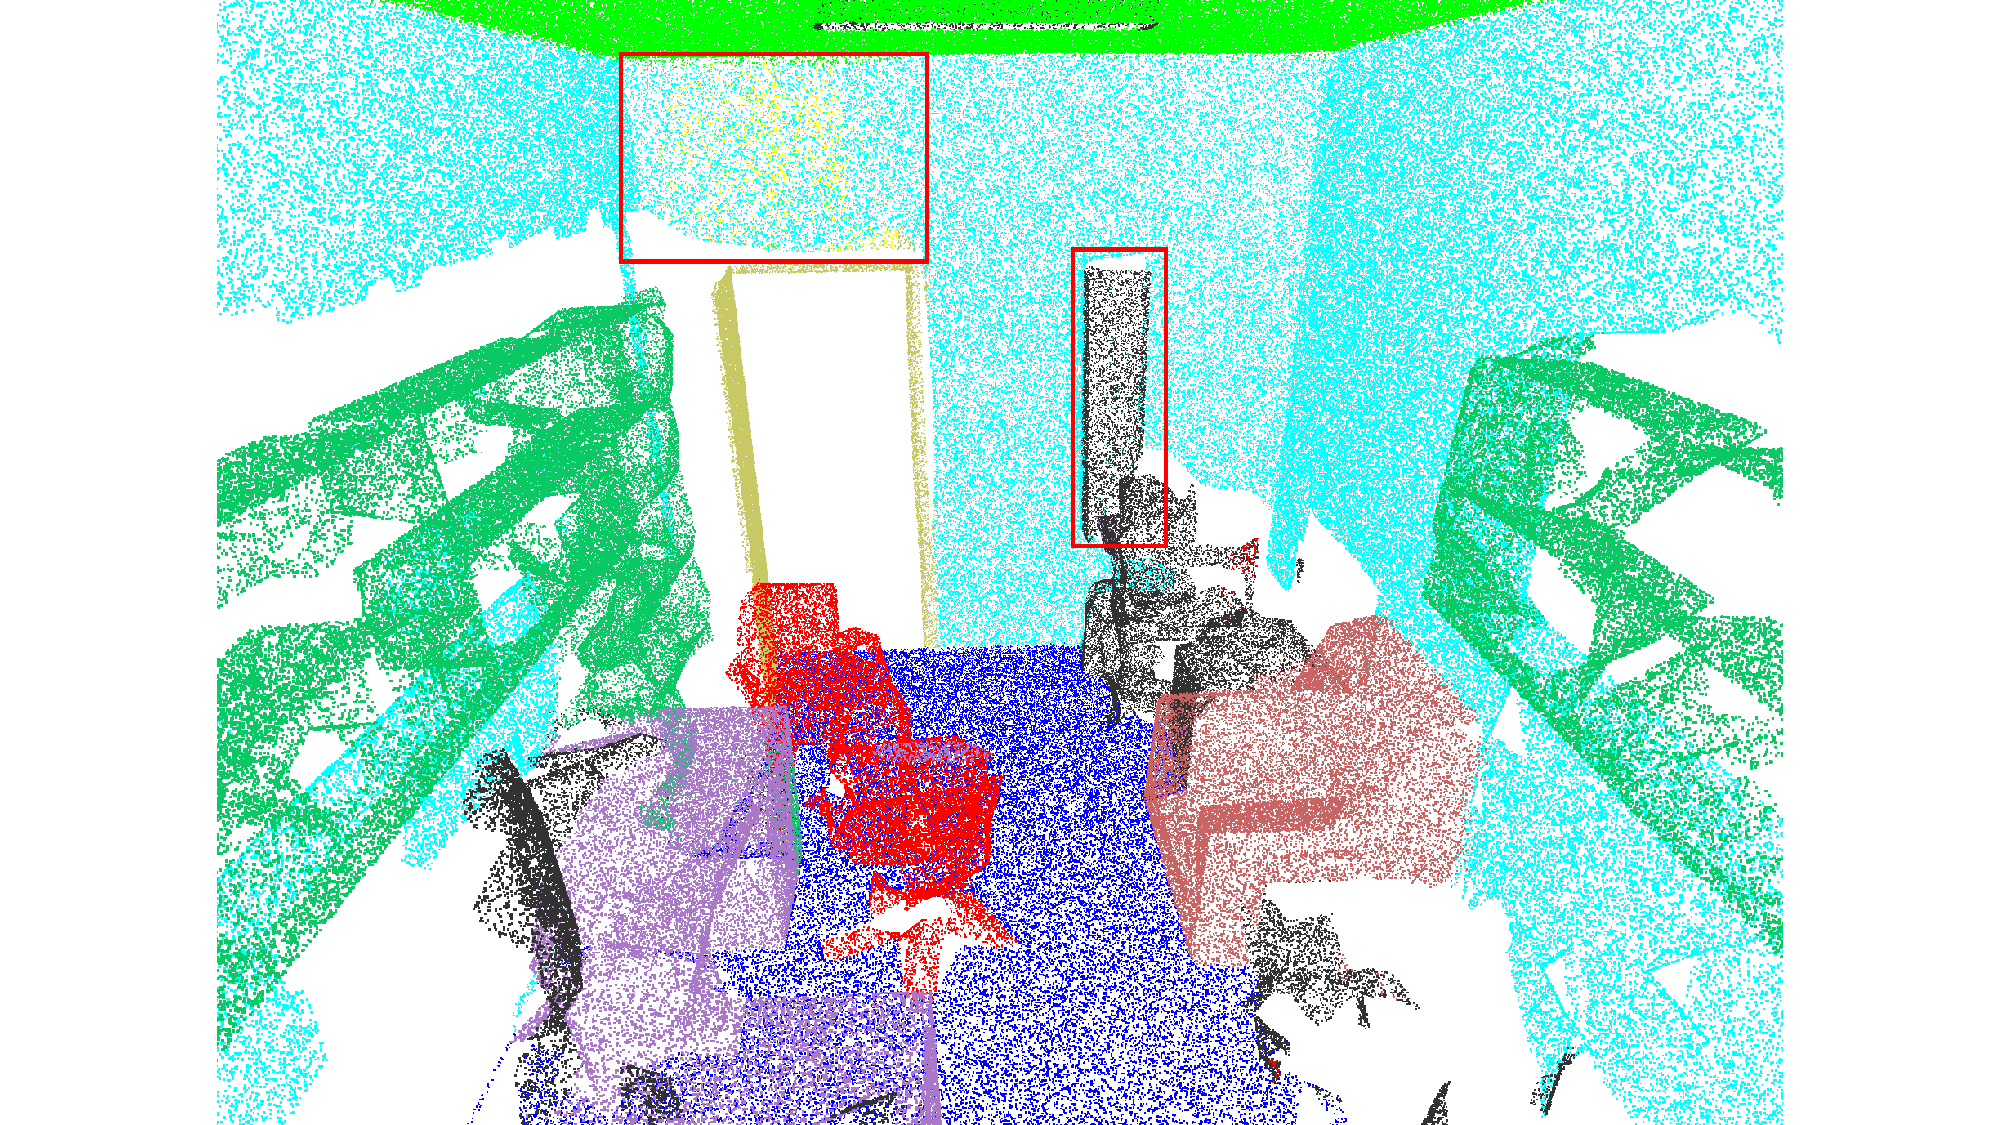
\includegraphics[width=\linewidth]{fig/S3DIS/PLT.pdf}
        % \caption*{\textbf{\#TP}:0.8M \textbf{\#OA}:82.75}
        \caption{PLT (Ours)}
        \label{fig:s3dis5}
    \end{subfigure}
    \hfill
    \begin{subfigure}{0.235\textwidth}
        \centering
        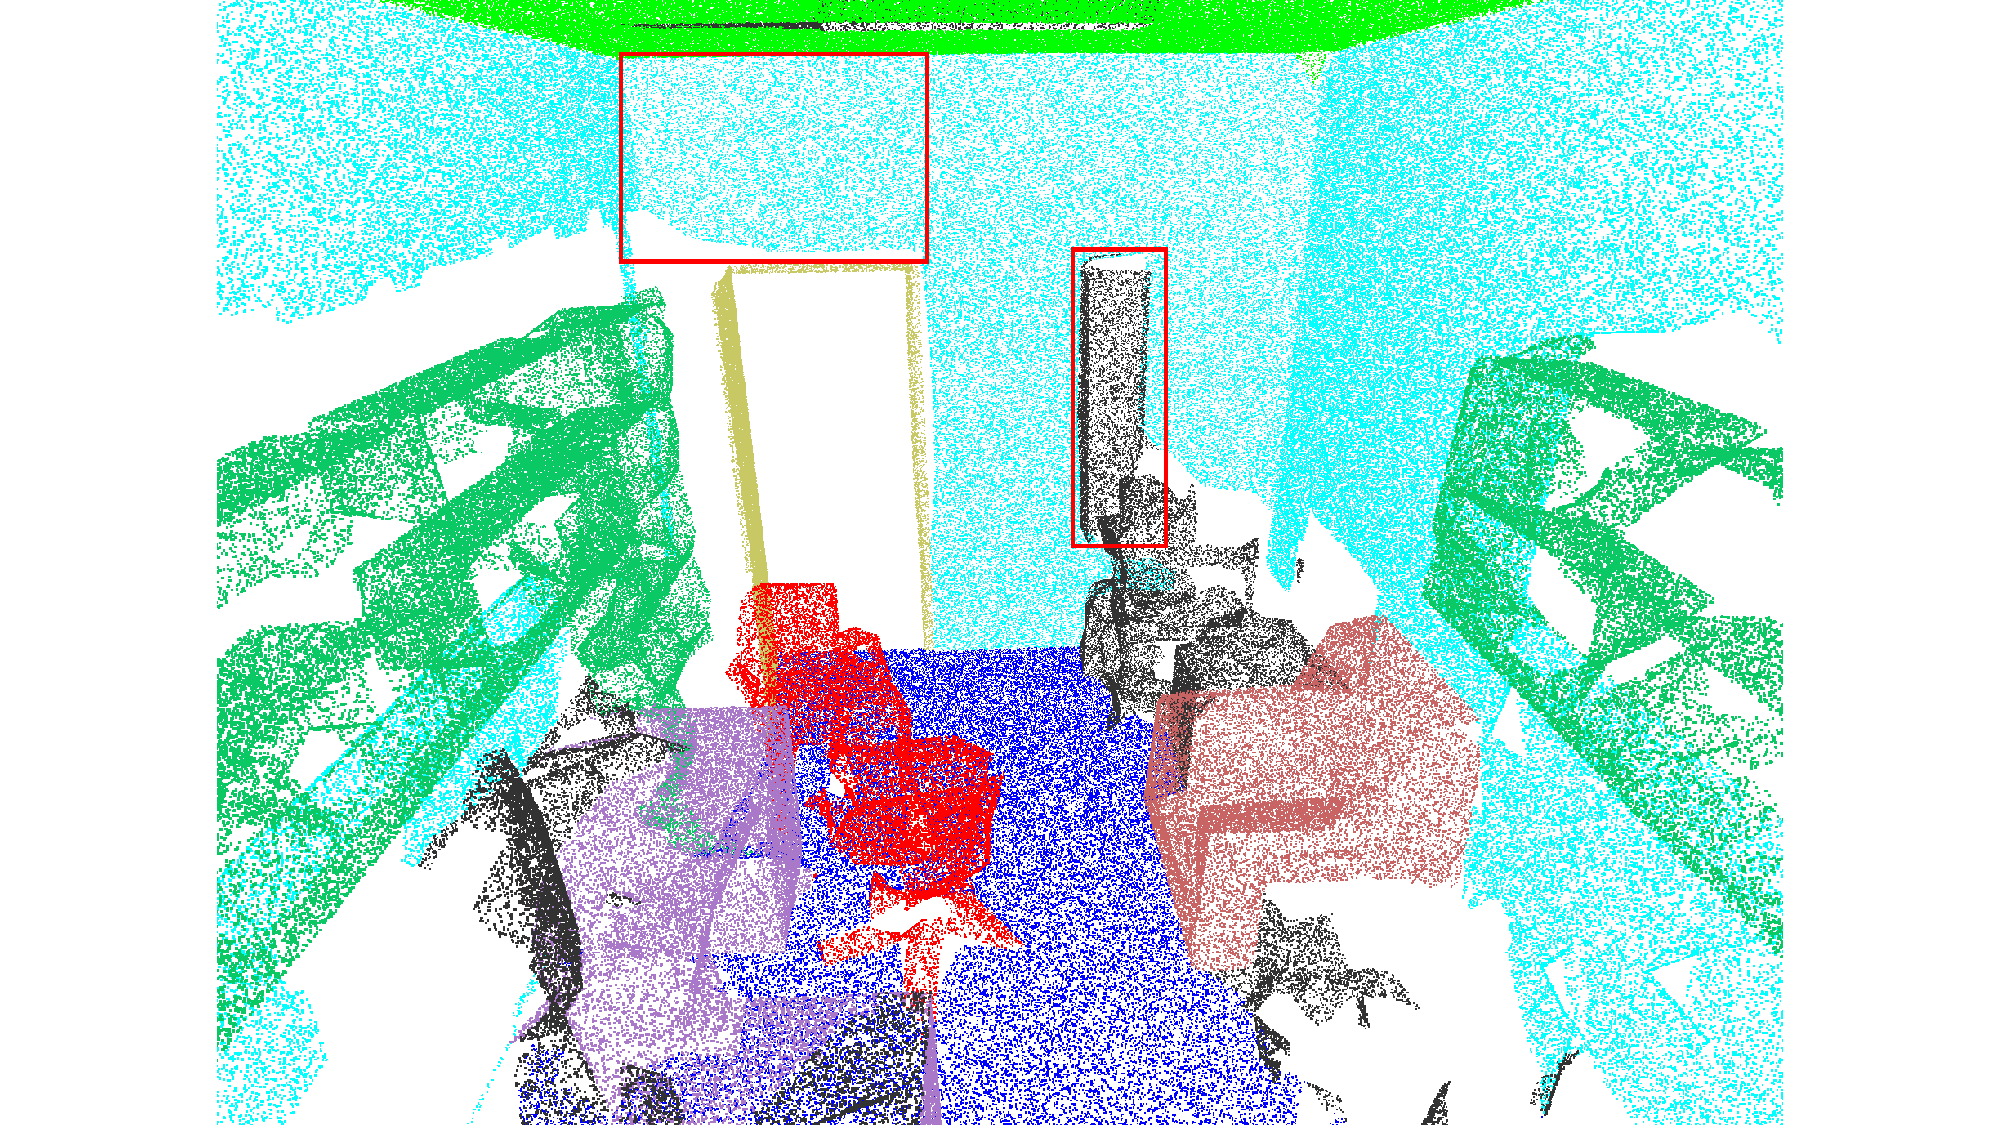
\includegraphics[width=\linewidth]{fig/S3DIS/GT.pdf}
        % \caption*{\textbf{\#TP}:0.6M \textbf{\#OA}:85.46}
        \caption{GT}
        \label{fig:s3dis6}
    \end{subfigure}
    \caption{The visualizations from the Area5 of S3DIS using a pre-trained PointMAE with different fine-tuning strategies.}
    \label{fig:s3dis}
\end{figure}

\begin{table}
\footnotesize
\setlength{\tabcolsep}{1.6mm}
\centering
\caption{The overall accuracy (\%) for classical fine-tuning strategies on three variants of ScanObjectNN~\cite{uy2019revisiting} is reported. `\#TP’ means the number of tunable parameters. Linear probing indicates head-tuned only.}
\label{tab:origin_finetuning}
\begin{tabular}{ lcccc }
\toprule
Tuning Strategy & \#TP(M) &OBJ\_BG &OBJ\_ONLY & PB\_T50\_RS \\
\midrule
Point-MAE~\cite{pang2022masked} & 22.1 & 90.02 & 88.29 & 85.18 \\
Linear probing & 0.3  & 87.26\dtplus{-2.76} & 84.85\dtplus{-3.44} & 75.99\dtplus{-9.19}\\
\midrule
+ Adapter~\cite{houlsby2019parameter} & 0.9  & 89.50\dtplus{-0.52} & 88.64\dplus{+0.35} & 83.93\dtplus{-1.25}\\
+ VPT~\cite{jia2022visual} & 0.4  & 87.26\dtplus{-2.76} & 87.09\dtplus{-1.20} &81.09\dtplus{-4.09} \\
+ LST~\cite{sung2022lst} & 0.8  & 89.67\dtplus{-0.25} & 89.67\dplus{+1.38} &82.75\dtplus{-2.43} \\
\bottomrule
\end{tabular}
\end{table}

\begin{table*}
    \centering
    \scriptsize
    \caption{Ablation on hyper-parameters and settings of LST, including the num of neighbors $K$, feature dim $d$ and the num of layers in Hierarchical Ladder Network (HLN). The tunable parameters (\#TP) and the overall accuracy (\%) on the hardest variant of ScanObjectNN\cite{uy2019revisiting} are reported.}
    \label{tab:ablation}
      \vspace{-5pt}
    \resizebox{0.95\linewidth}{!}{
    \begin{subtable}[t]{0.25\linewidth} % 0.245
        \centering
        \scriptsize
         \setlength{\tabcolsep}{1.2mm} % 1.2mm
        \caption{Ablation on $K$ in HLN.}
        \label{tab:k}
        \begin{tabular}{ccc}
           \toprule
            $K$ & \#TP (M) & PB\_T50\_RS \\
            \midrule
            \text{[16, 16, 16]} & 0.60 & 84.46 \\
            \text{[4, 4, 4]} & 0.60 & 84.66 \\
            \text{[4, 8, 16]} & 0.60 & 84.91 \\
            \rowcolor{linecolor!40} \text{[16, 8, 4]} & 0.60 & \textbf{85.46} \\
            \bottomrule
        \end{tabular}
    \end{subtable}

    \begin{subtable}[t]{0.4\linewidth} % 0.235
        \centering
        \scriptsize
         \setlength{\tabcolsep}{1.2mm} % 0.2mm
        \caption{Ablation on $d$ in HLN.}
        \label{tab:dim}
        \begin{tabular}{ccc}
            \toprule
            Feature Dim & \#TP (M) & PB\_T50\_RS \\
            \midrule
            \text{[8, 16, 32, 64]} & 0.46 & 83.17 \\
            \rowcolor{linecolor!40} \text{[16, 32, 64, 128]} & 0.60 & \textbf{85.46} \\
            \text{[32, 64, 128, 256]} & 1.00 & 84.25 \\
            \bottomrule
        \end{tabular}
    \end{subtable}

    \begin{subtable}[t]{0.24\linewidth} % 0.22
    \setlength{\tabcolsep}{1.0mm} % 1.3mm
        \centering
         \scriptsize
        \caption{Ablation on the num of layers.}
        \label{tab:layer}
     
        \begin{tabularx}{\textwidth}{ccc}
            \toprule
            Layer num & \#TP (M) & PB\_T50\_RS \\
            \midrule
            1 & 0.40 & 83.55 \\
            2 & 0.45 & 84.84 \\
            \rowcolor{linecolor!40}3 & 0.60 & \textbf{85.46} \\
            4 & 1.09 & 85.05 \\
            \bottomrule
        \end{tabularx}
    \end{subtable}
}
% \vspace{-10pt}
\end{table*}

\subsection{3D Dense Prediction Task}
For dense prediction tasks, including part segmentation and semantic segmentation, we adopt a prediction head similar to that of PointNext, allowing us to effectively utilize multi-scale information and enhance performance while maintaining a low number of trainable parameters.

We validate the effectiveness of PLT on the ShapeNetPart dataset~\cite{yi2016scalable}. As shown in Tab.~\ref{tab:segmentation}, PLT achieves results comparable to other methods in terms of instance-level mIoU (Inst. mIoU) while achieving notable improvements in class-level mIoU (Cls. mIoU). Specifically, PLT improves Cls. mIoU on PointBERT by 0.5\% over DAPT, demonstrating its effectiveness in capturing fine-grained details.

To evaluate PLT in the semantic segmentation task, we use the S3DIS dataset~\cite{armeni20163d}, with results presented in Tab.~\ref{tab:semantic_segmentation}. When using ACT as the baseline, PLT shows significant improvements of 7.2\%, 4.7\%, 4.8\%, and 1.9\% over IDPT, PointPEFT, DAPT, and PointGST, respectively. Likewise, with PointMAE as the baseline, PLT consistently outperforms other methods, further validating its effectiveness in dense prediction tasks. Additionally, as illustrated in Fig.~\ref{fig:s3dis}, the semantic segmentation results on the S3DIS dataset demonstrate that PLT achieves clearer segmentation boundaries and fewer misclassifications compared to other methods.


\begin{table}
  \centering
  \scriptsize
  \setlength{\tabcolsep}{0.6mm}
  \caption{Part segmentation on the ShapeNetPart~\cite{yi2016scalable}. The mIoU for all classes (Cls.) and for all instances (Inst.) are reported. \#TP represents the tunable parameters. \textcolor{red}{$^*$} denotes reproduced results.}
    \vspace{-10pt}
    \begin{tabular}{lcccc}
    \toprule
    Methods & Reference & \#TP (M)& Cls. mIoU (\%) & Inst. mIoU (\%) \\
    \midrule
    \multicolumn{5}{c}{\textit{Supervised Learning Only}} \\
    \midrule
    PointNet~\cite{qi2017pointnet}  & CVPR 17  &- & 80.39 & 83.7 \\
    PointNet++~\cite{qi2017pointnet++}    & NeurIPS 17 &-  & 81.85 & 85.1 \\
    DGCNN~\cite{wang2019dynamic}  & TOG 19 & - & 82.33 & 85.2 \\
    APES~\cite{wu2023attention} & CVPR 23& - & 83.67 & 85.8\\
    \midrule
    \multicolumn{5}{c}{\textit{ Self-Supervised Representation Learning (Full fine-tuning)}} \\
    \midrule
    % Transformer \cite{} & & 27.09 & 83.42 & 85.1 \\
    OcCo~\cite{wang2021unsupervised}  & ICCV 21 & 27.09 & 83.42 & 85.1 \\
    MaskPoint~\cite{liu2022masked}  & ECCV 22 & - & 84.60 & 86.0 \\
    Point-BERT~\cite{yu2022point}  & CVPR 22 & 27.09 & 84.11 & 85.6 \\
    Point-MAE~\cite{pang2022masked}  & ECCV 22 & 27.06 & 84.19 & 86.1 \\ 
    ACT~\cite{dong2022autoencoders}  & ICLR 23 &  27.06 & 84.66 & 86.1 \\
    \midrule
    \multicolumn{5}{c}{\textit{ Self-Supervised Representation Learning (Efficient fine-tuning)}} \\
    \midrule
    Point-BERT~\cite{yu2022point} (baseline) &  CVPR 22 & 27.09 & 84.11 & 85.6 \\ 
    + IDPT\textcolor{red}{$^*$}~\cite{zha2023instance} & ICCV 23 & 5.69  & 83.50  & 85.3  \\
    + DAPT~\cite{zhou2024dynamic} & CVPR 24 & 5.65  & 83.83 & 85.5 \\
    % + PointGST~\cite{liang2024parameter} & Arxiv 24 & 5.58  & \textbf{83.87} & 85.7 \\
    \rowcolor{linecolor!40}+ PLT (\textbf{ours})& - & \textbf{2.08}  & \textbf{83.85} & \textbf{86.0} \\
    \midrule
    Point-MAE~\cite{pang2022masked} (baseline) &  ECCV 22 & 27.06 & 84.19 & 86.1 \\ 
    + IDPT~\cite{zha2023instance} & ICCV 23 & 5.69  & 83.79  & 85.7  \\
    + DAPT~\cite{zhou2024dynamic} & CVPR 24 & 5.65  & 84.01 & 85.7 \\
    % + PPT~\cite{zhang2024positional} & Arxiv 24 & 5.62  & \textbf{84.07} & 85.7 \\
    % + PointGST~\cite{liang2024parameter} & Arxiv 24 & 5.59  & 83.98 & 85.8 \\
    \rowcolor{linecolor!40}+ PLT (\textbf{ours})& - & \textbf{2.08}  & 83.90 & \textbf{85.9} \\
    \bottomrule
    \end{tabular}
    % \vspace{-10pt}
  \label{tab:segmentation}
\end{table}

\begin{figure*}[htbp]
    \centering

    % 第一行左侧的竖排标签
    \begin{minipage}{0.09\textwidth}
        \centering
        Full
        Fine-tuning
    \end{minipage}
    \hfill
    % 第一行图片
    \begin{minipage}{0.22\textwidth}
        \centering
        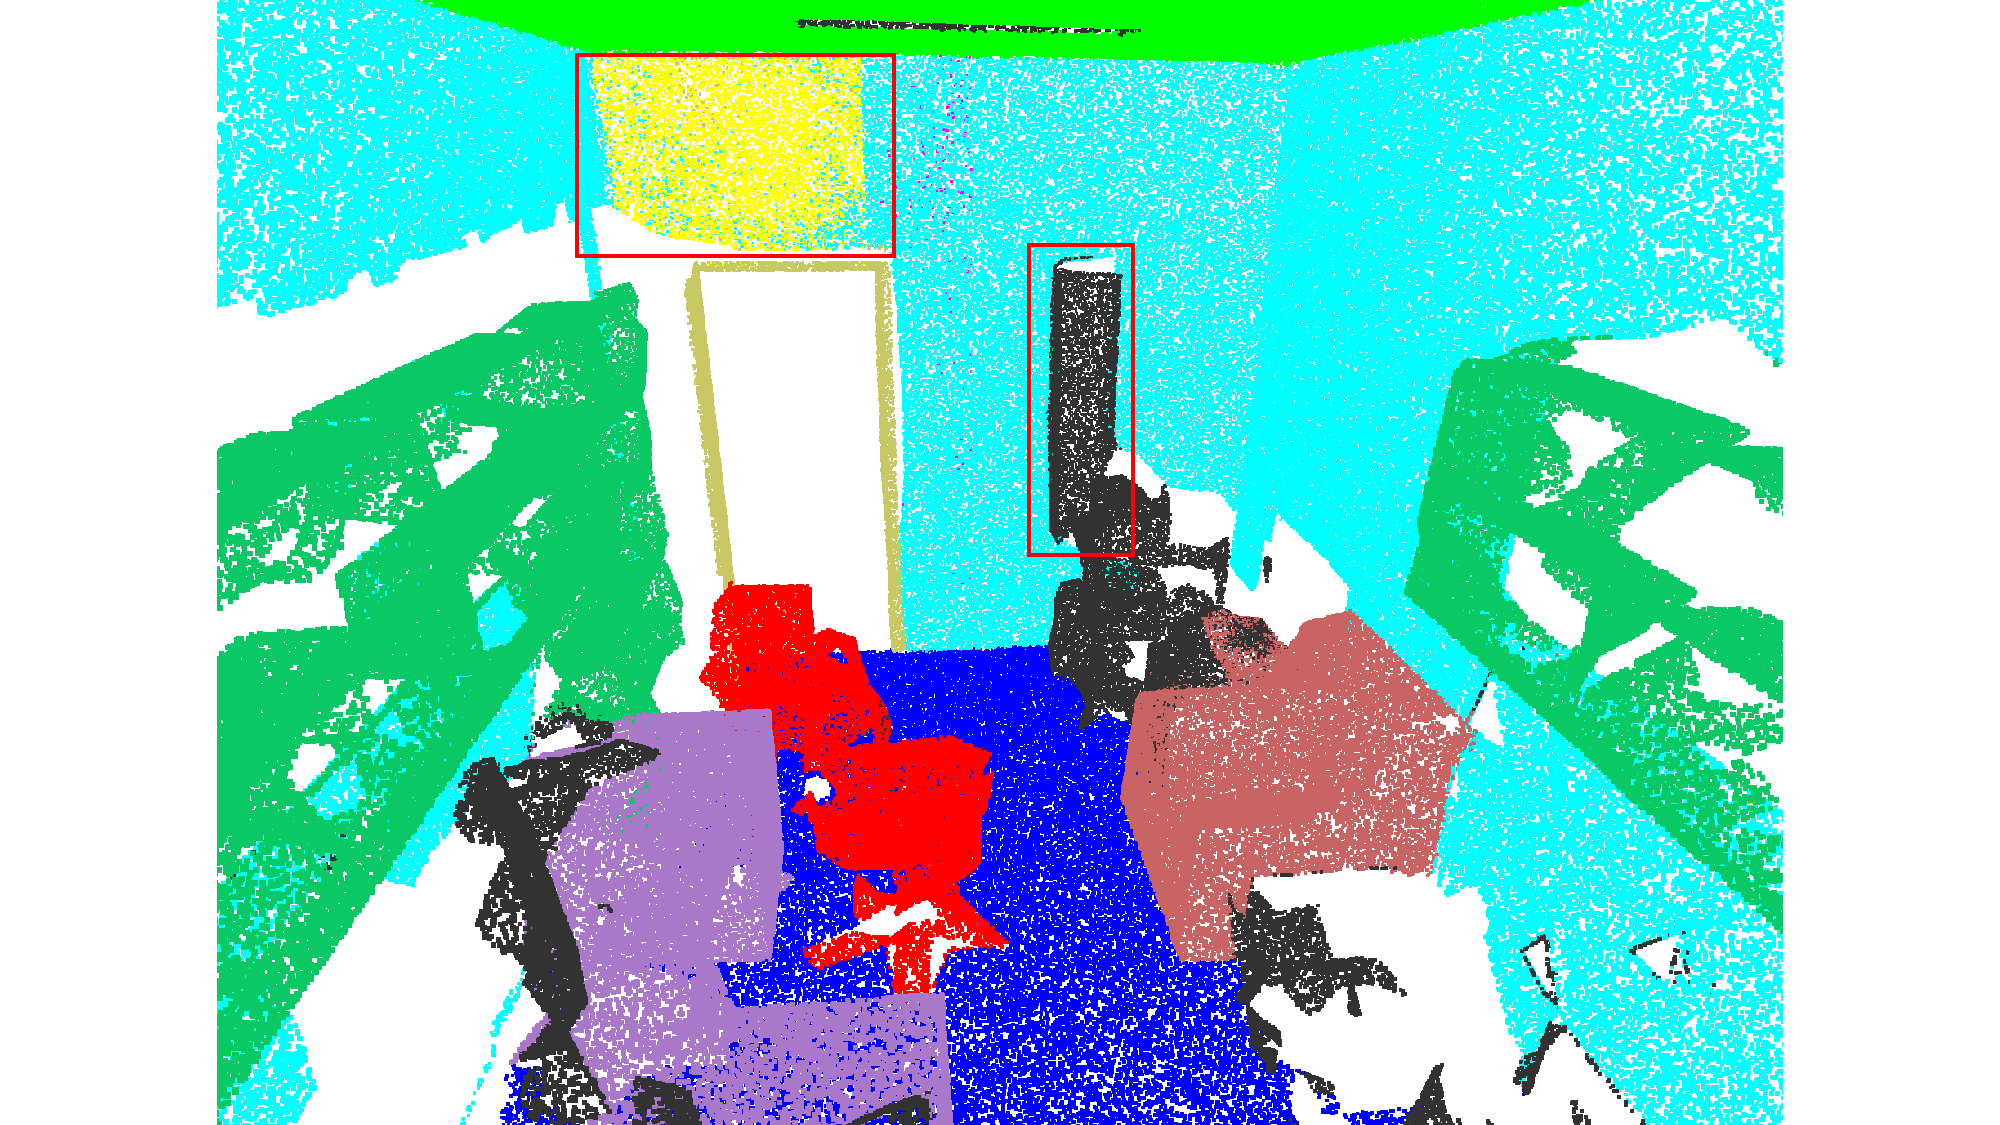
\includegraphics[width=\textwidth]{fig/supplement/semantic_segmentation/office_9/PT_office_9.pdf}
    \end{minipage}
    \hfill
    \begin{minipage}{0.22\textwidth}
        \centering
        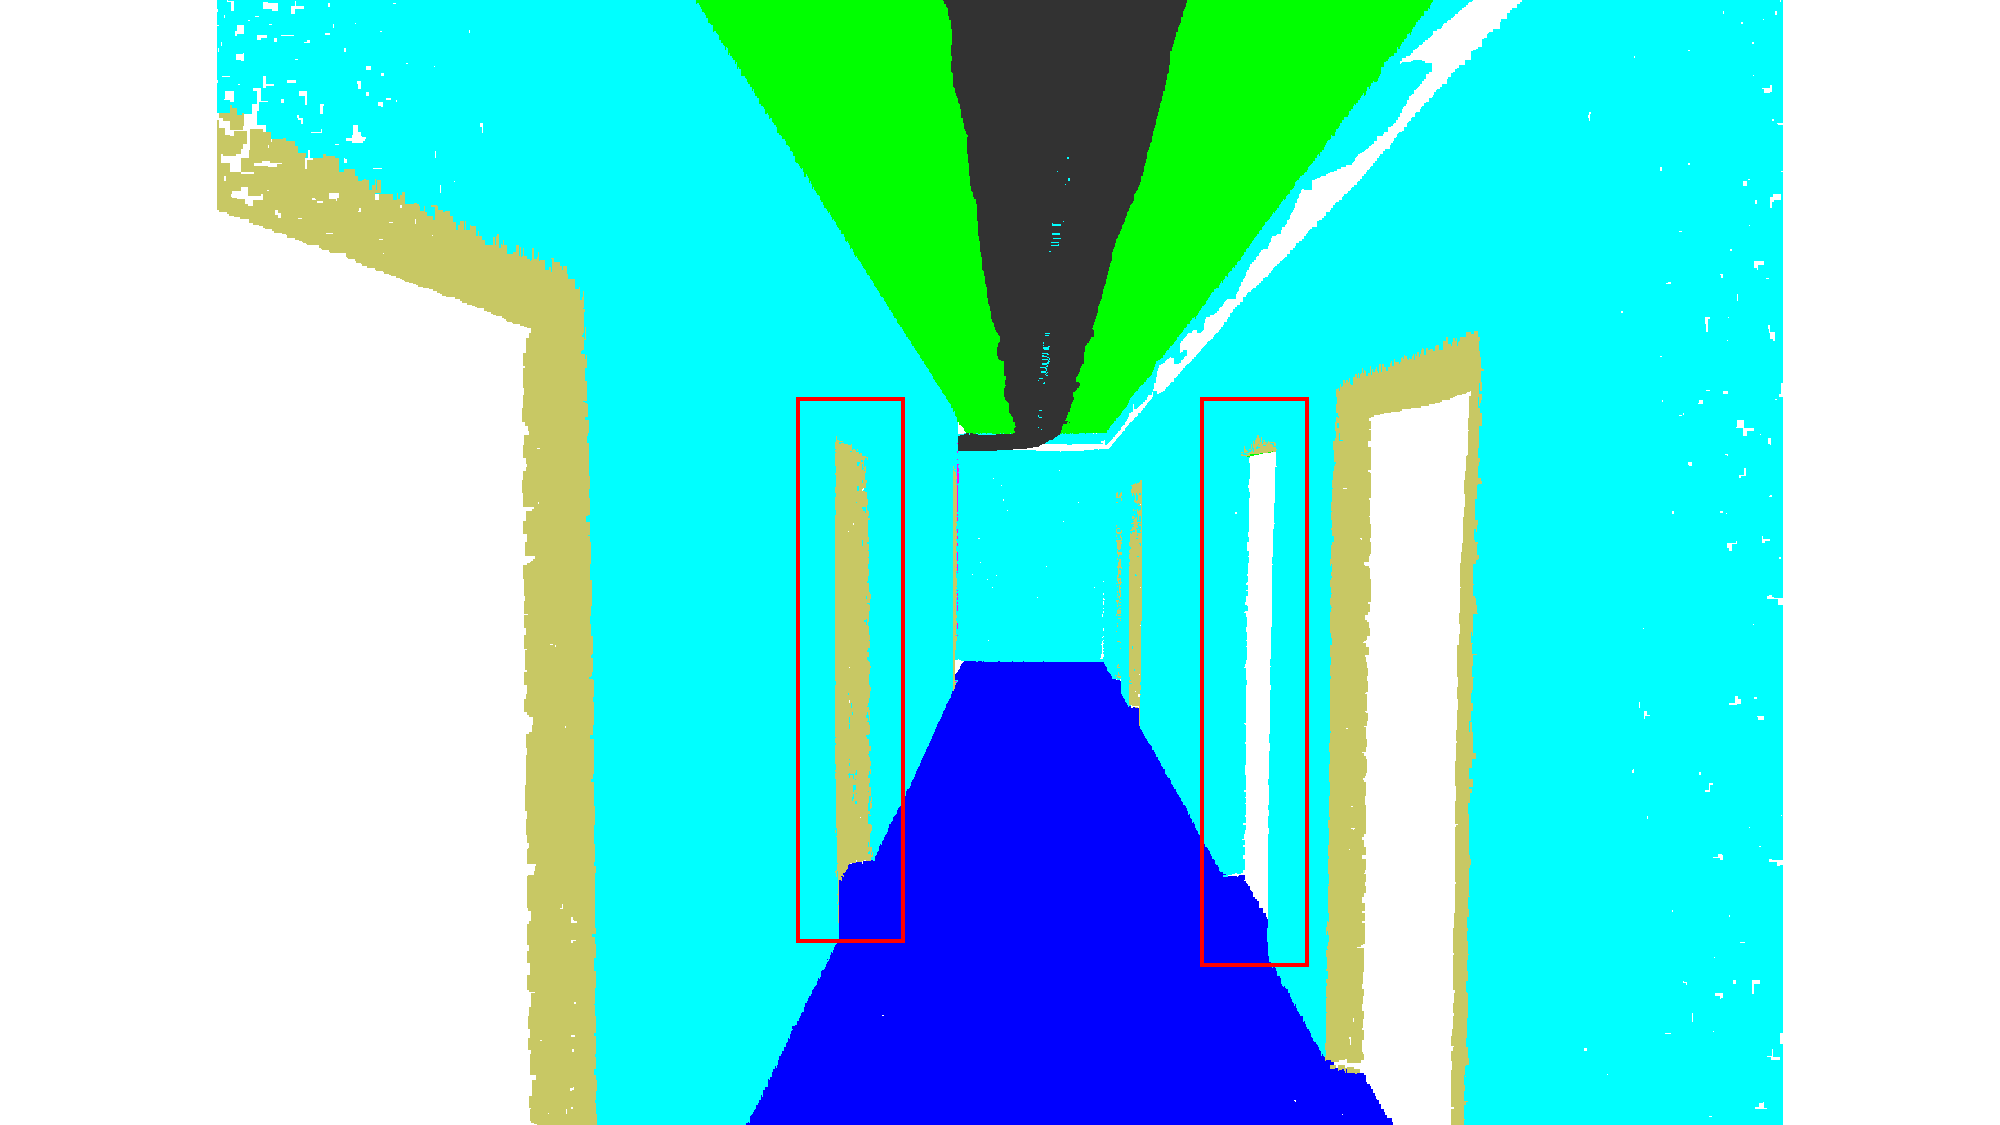
\includegraphics[width=\textwidth]{fig/supplement/semantic_segmentation/hallway_10/PT_hallway_10.pdf} % 替换为你的图片路径
    \end{minipage}
    \hfill
    \begin{minipage}{0.22\textwidth}
        \centering
        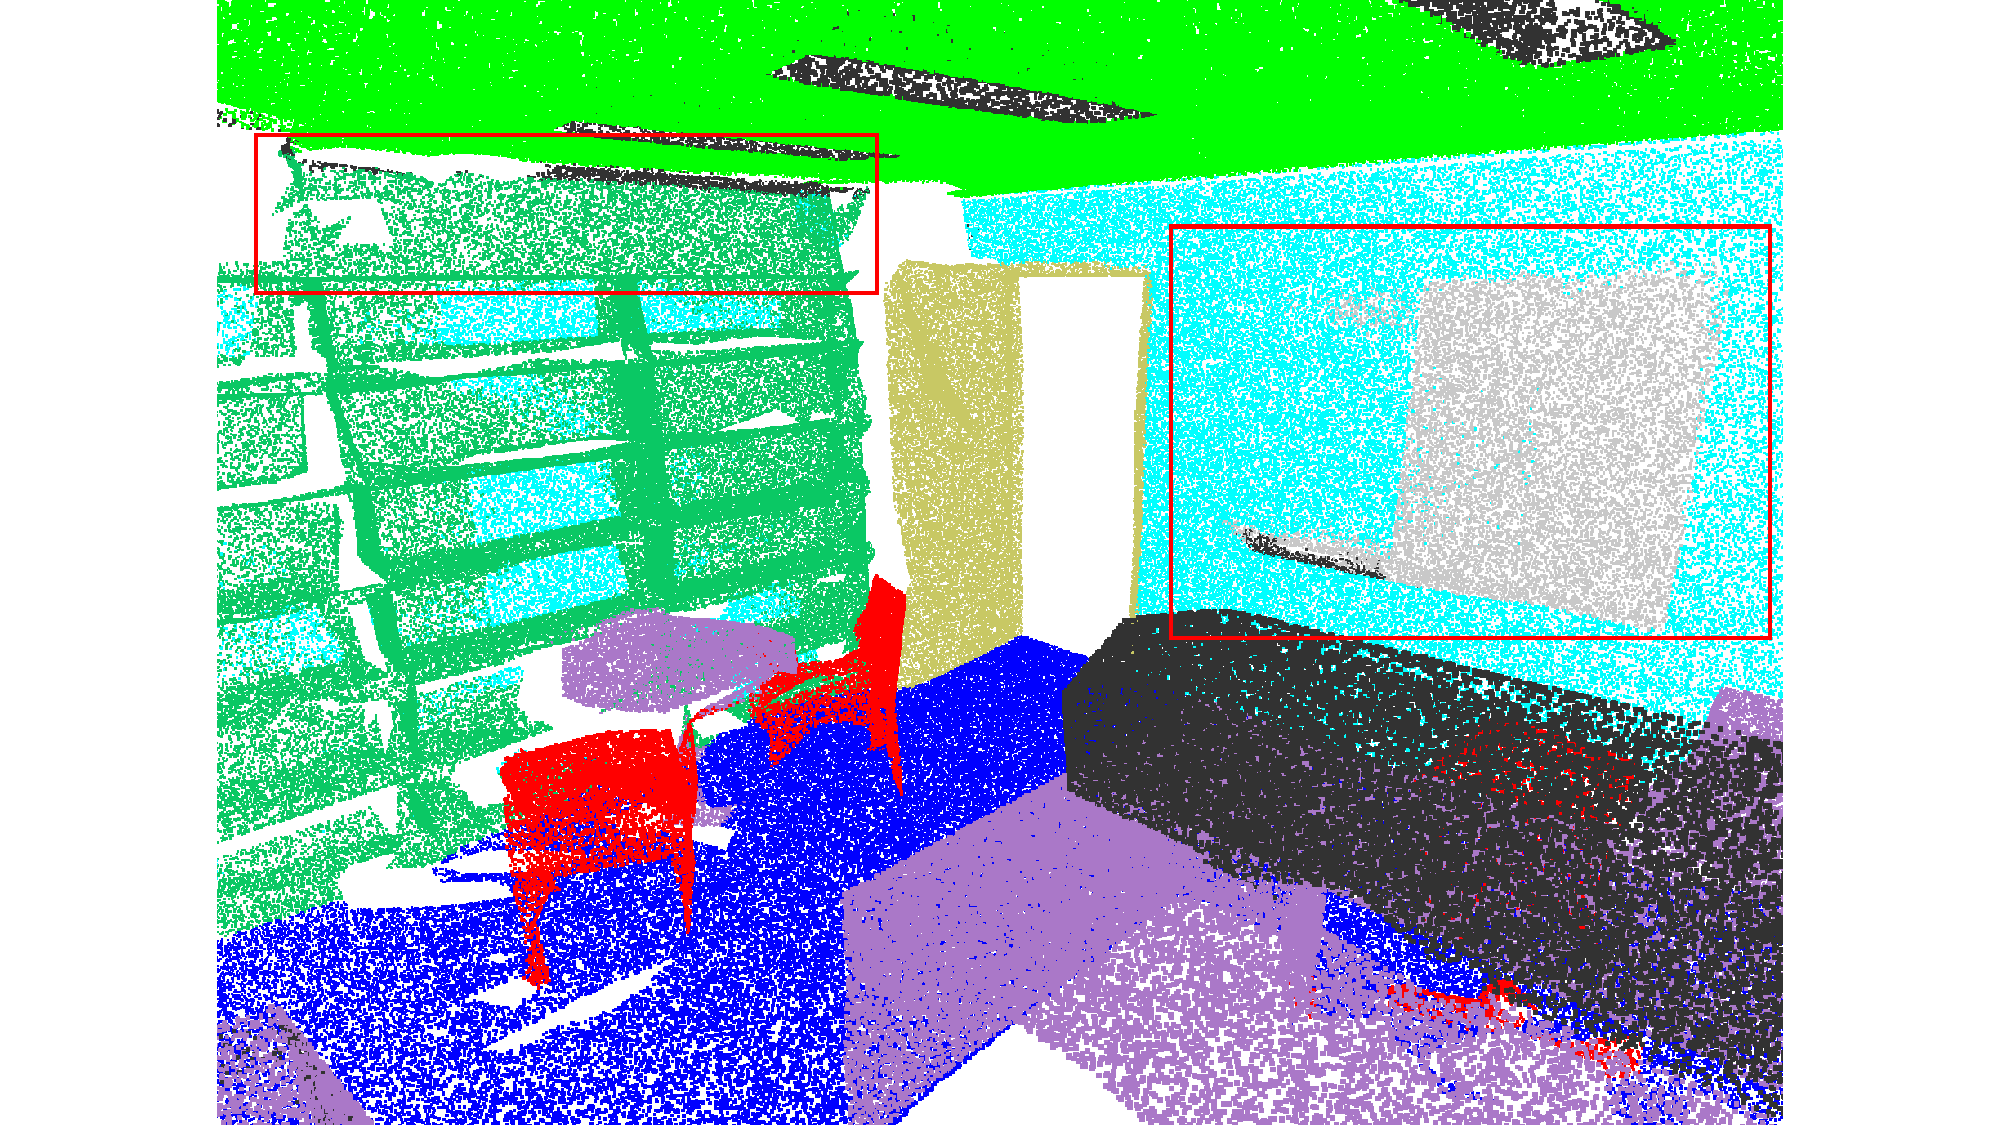
\includegraphics[width=\textwidth]{fig/supplement/semantic_segmentation/office_35/PT_office_35.pdf}
    \end{minipage}
    \hfill
    \begin{minipage}{0.22\textwidth}
        \centering
        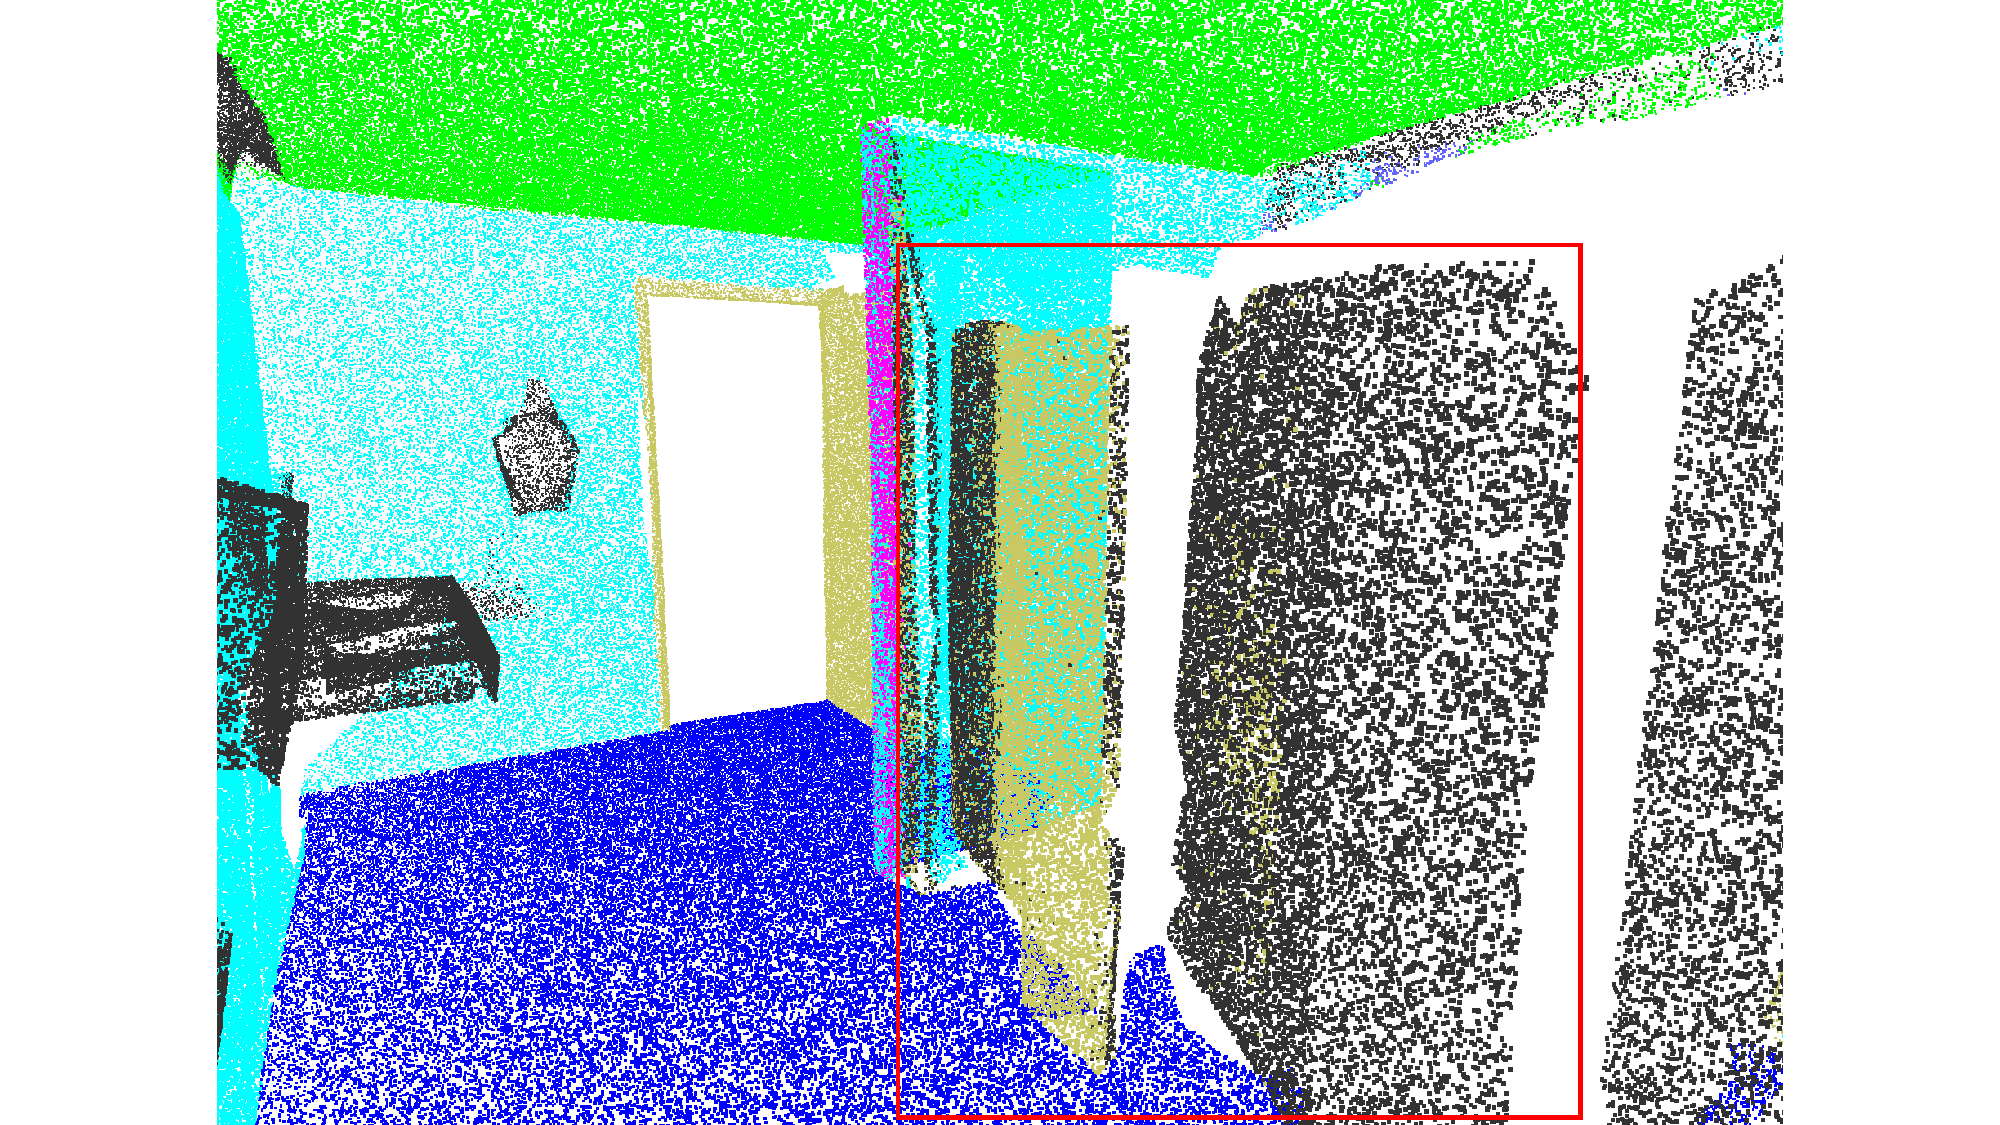
\includegraphics[width=\textwidth]{fig/supplement/semantic_segmentation/wc_2/PT_wc_2.pdf}
    \end{minipage}
    \hfill

    % 换行
    \vspace{0.5em}

    % 第二行左侧的竖排标签
    \begin{minipage}{0.09\textwidth}
        \centering
        DAPT
    \end{minipage}
    \hfill
    % 第二行图片
    \begin{minipage}{0.22\textwidth}
        \centering
        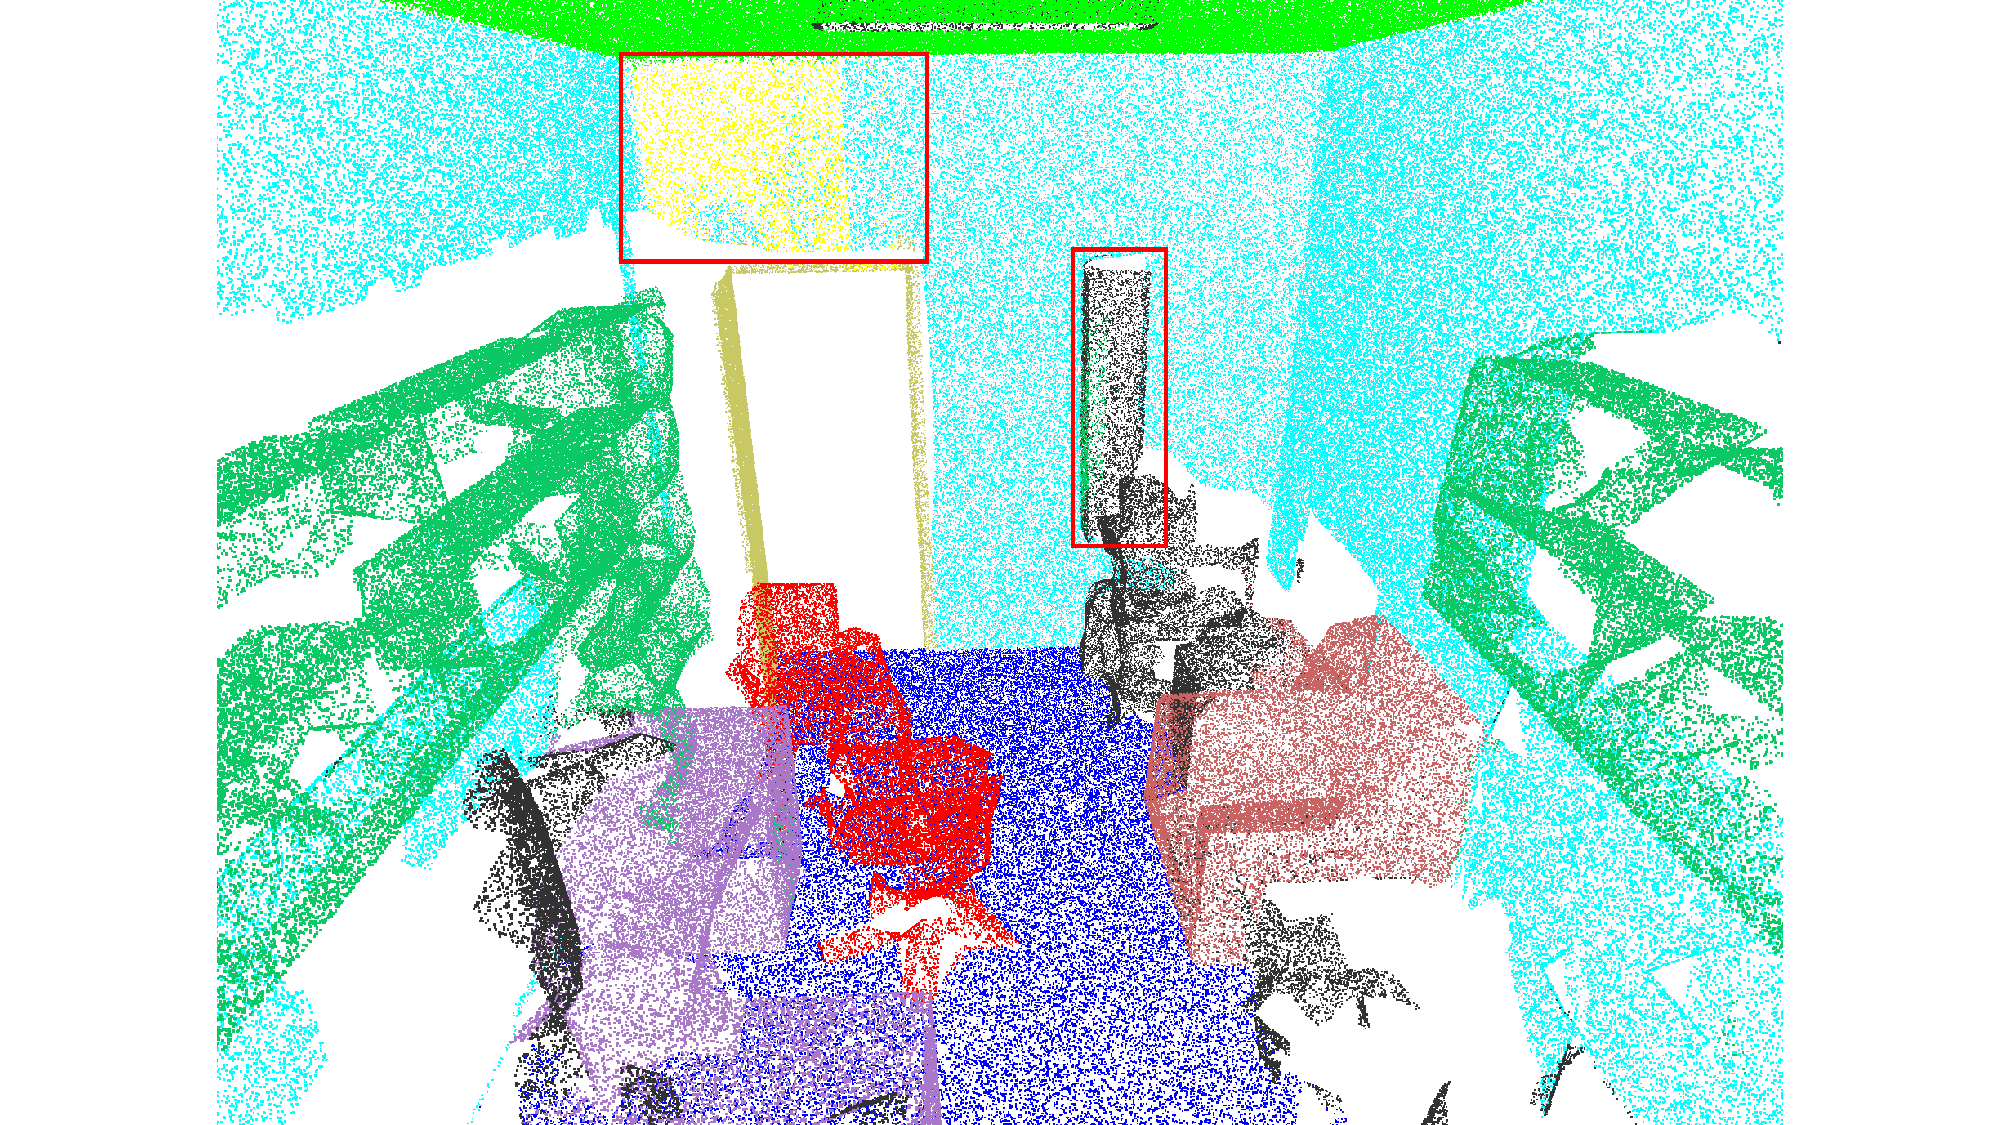
\includegraphics[width=\textwidth]{fig/supplement/semantic_segmentation/office_9/DAPT_office_9.pdf}
    \end{minipage}
    \hfill
    \begin{minipage}{0.22\textwidth}
        \centering
        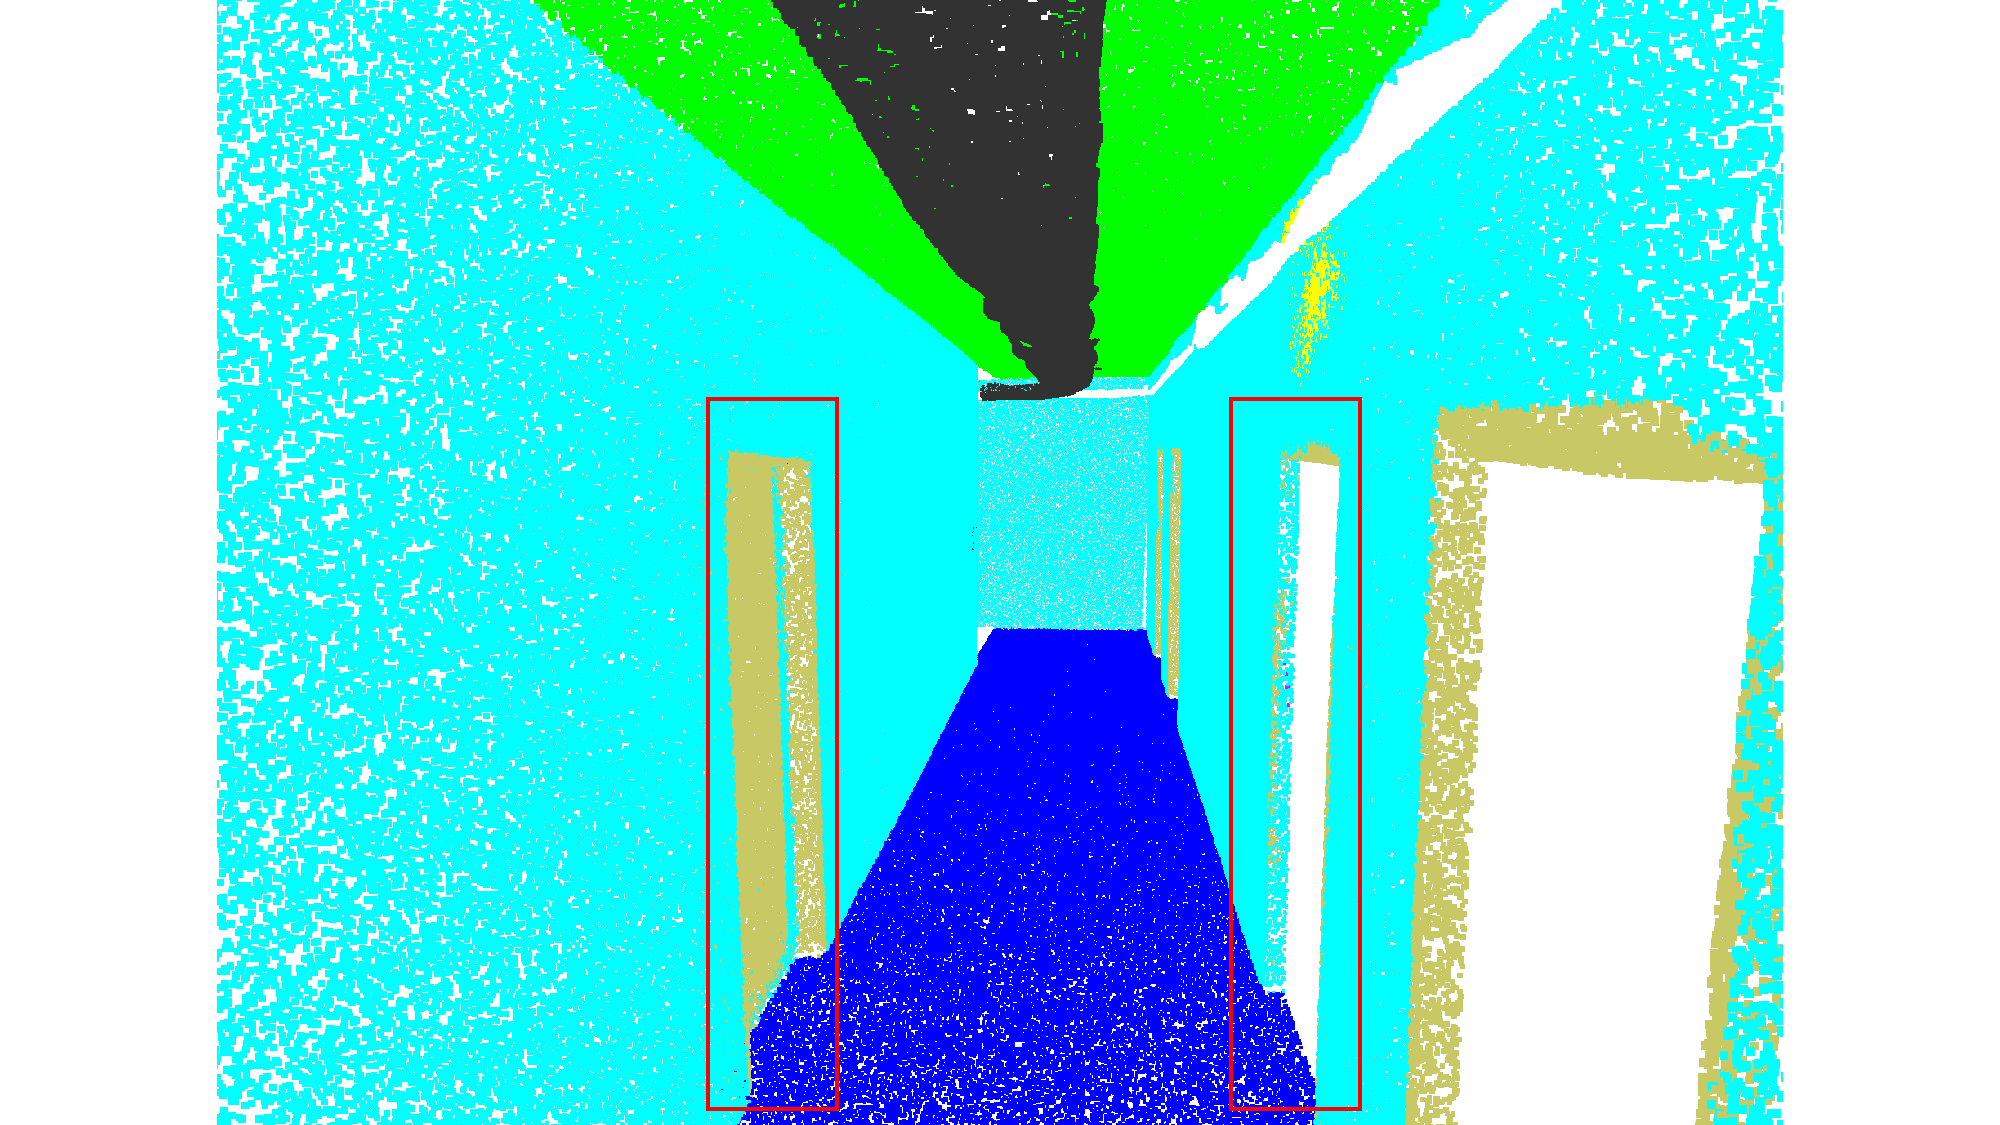
\includegraphics[width=\textwidth]{fig/supplement/semantic_segmentation/hallway_10/DAPT_hallway_10.pdf}
    \end{minipage}
    \hfill
    \begin{minipage}{0.22\textwidth}
        \centering
        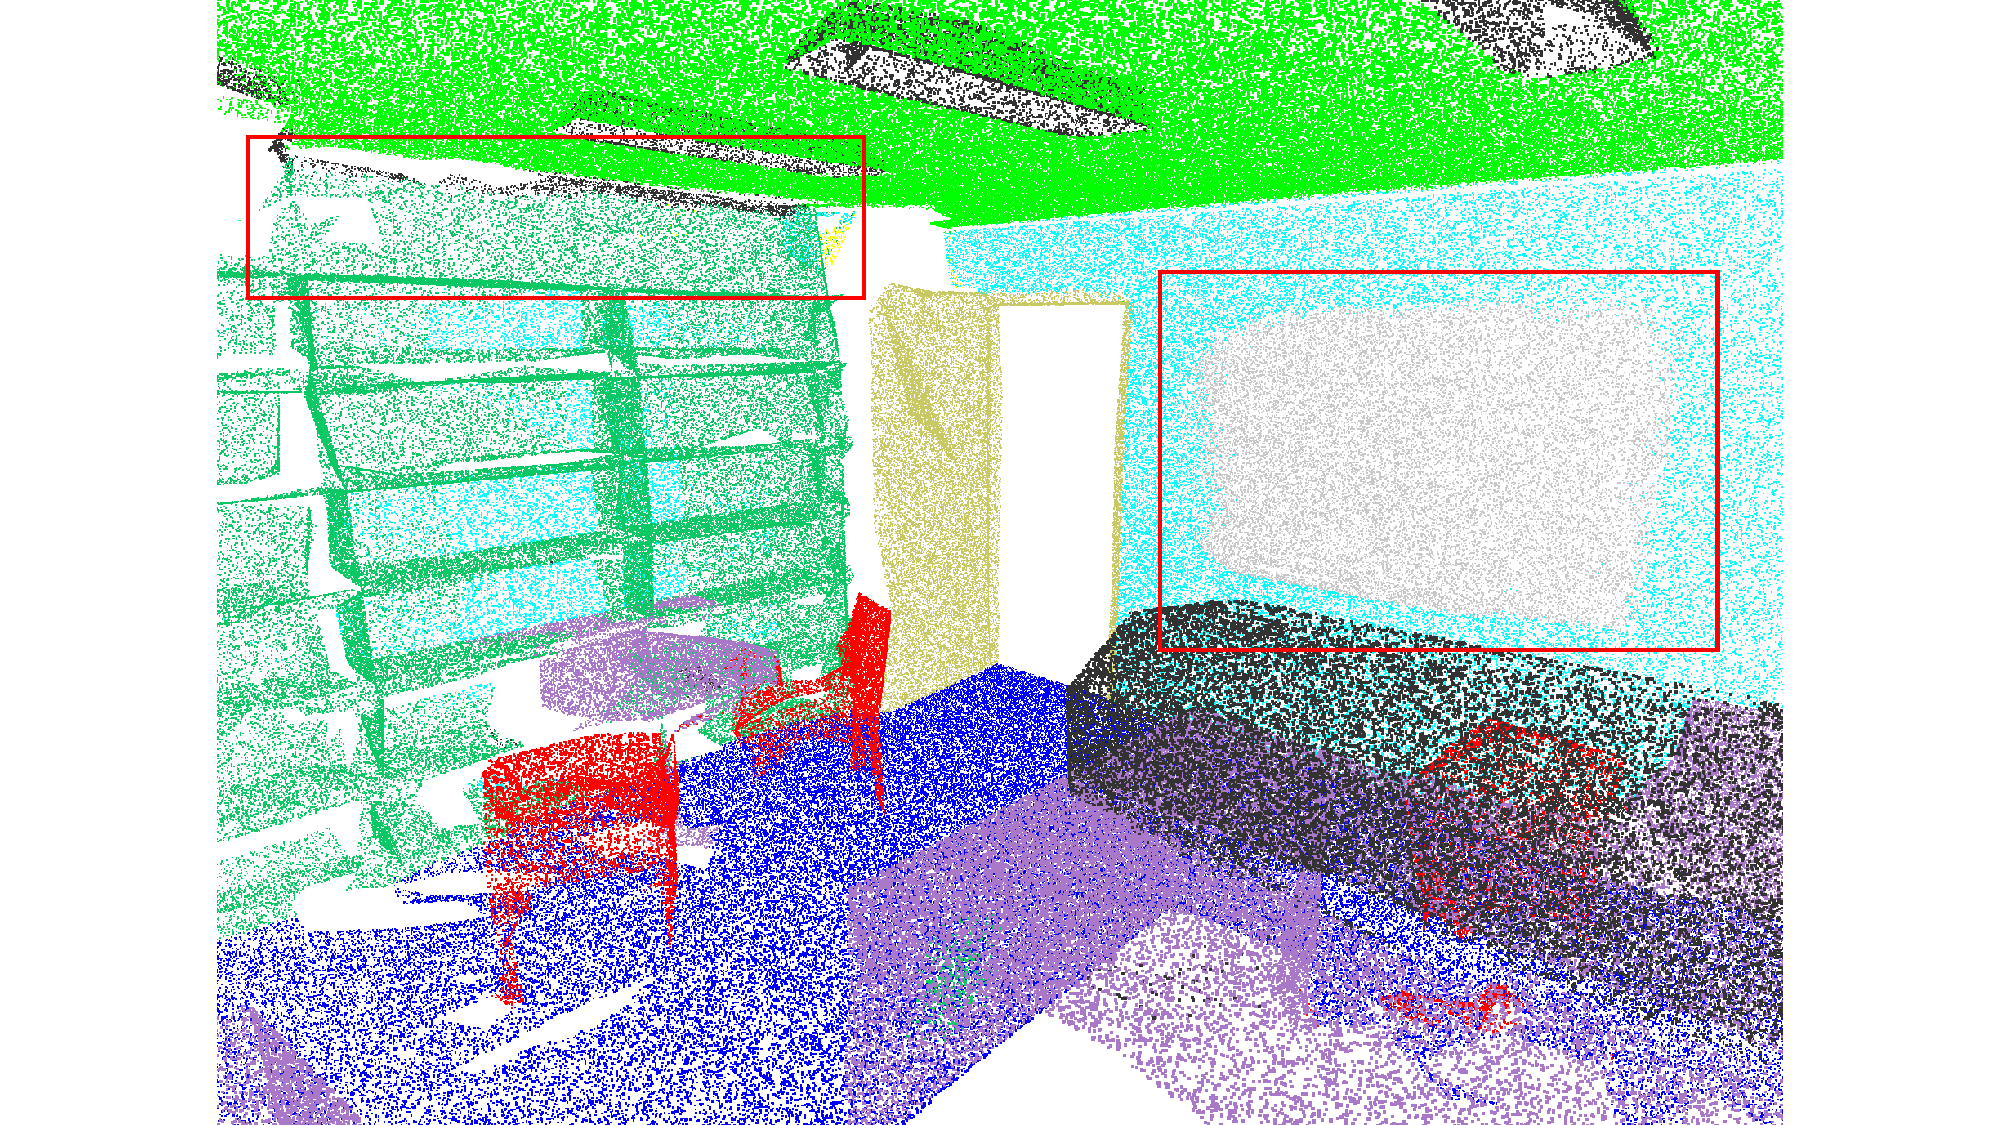
\includegraphics[width=\textwidth]{fig/supplement/semantic_segmentation/office_35/DAPT_office_35.pdf}
    \end{minipage}
    \hfill
    \begin{minipage}{0.22\textwidth}
        \centering
        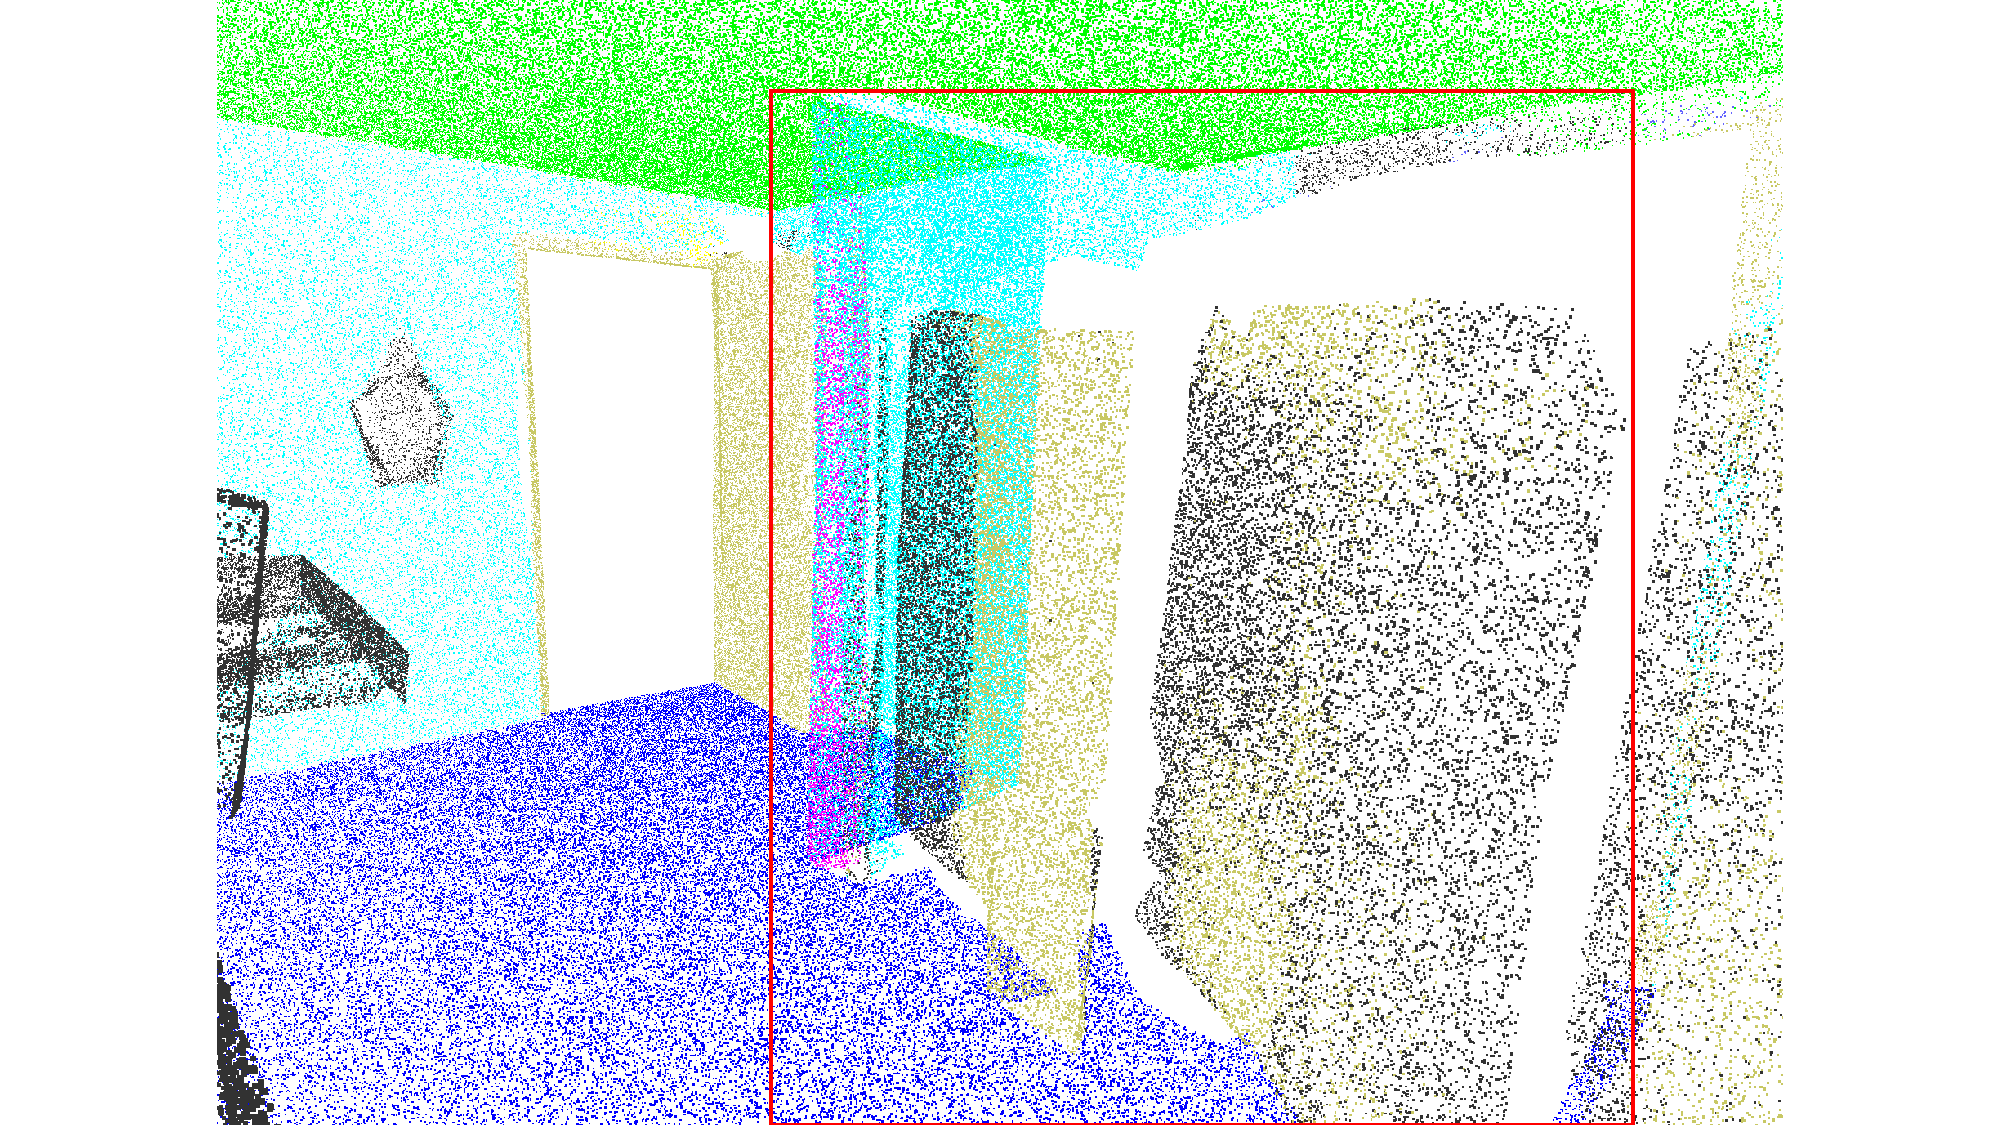
\includegraphics[width=\textwidth]{fig/supplement/semantic_segmentation/wc_2/DAPT_wc_2.pdf}
    \end{minipage}
    \hfill

    % 换行
    \vspace{0.5em}

    % 第三行左侧的竖排标签
    \begin{minipage}{0.09\textwidth}
        \centering
        IDPT
    \end{minipage}
    \hfill
    % 第三行图片
    \begin{minipage}{0.22\textwidth}
        \centering
        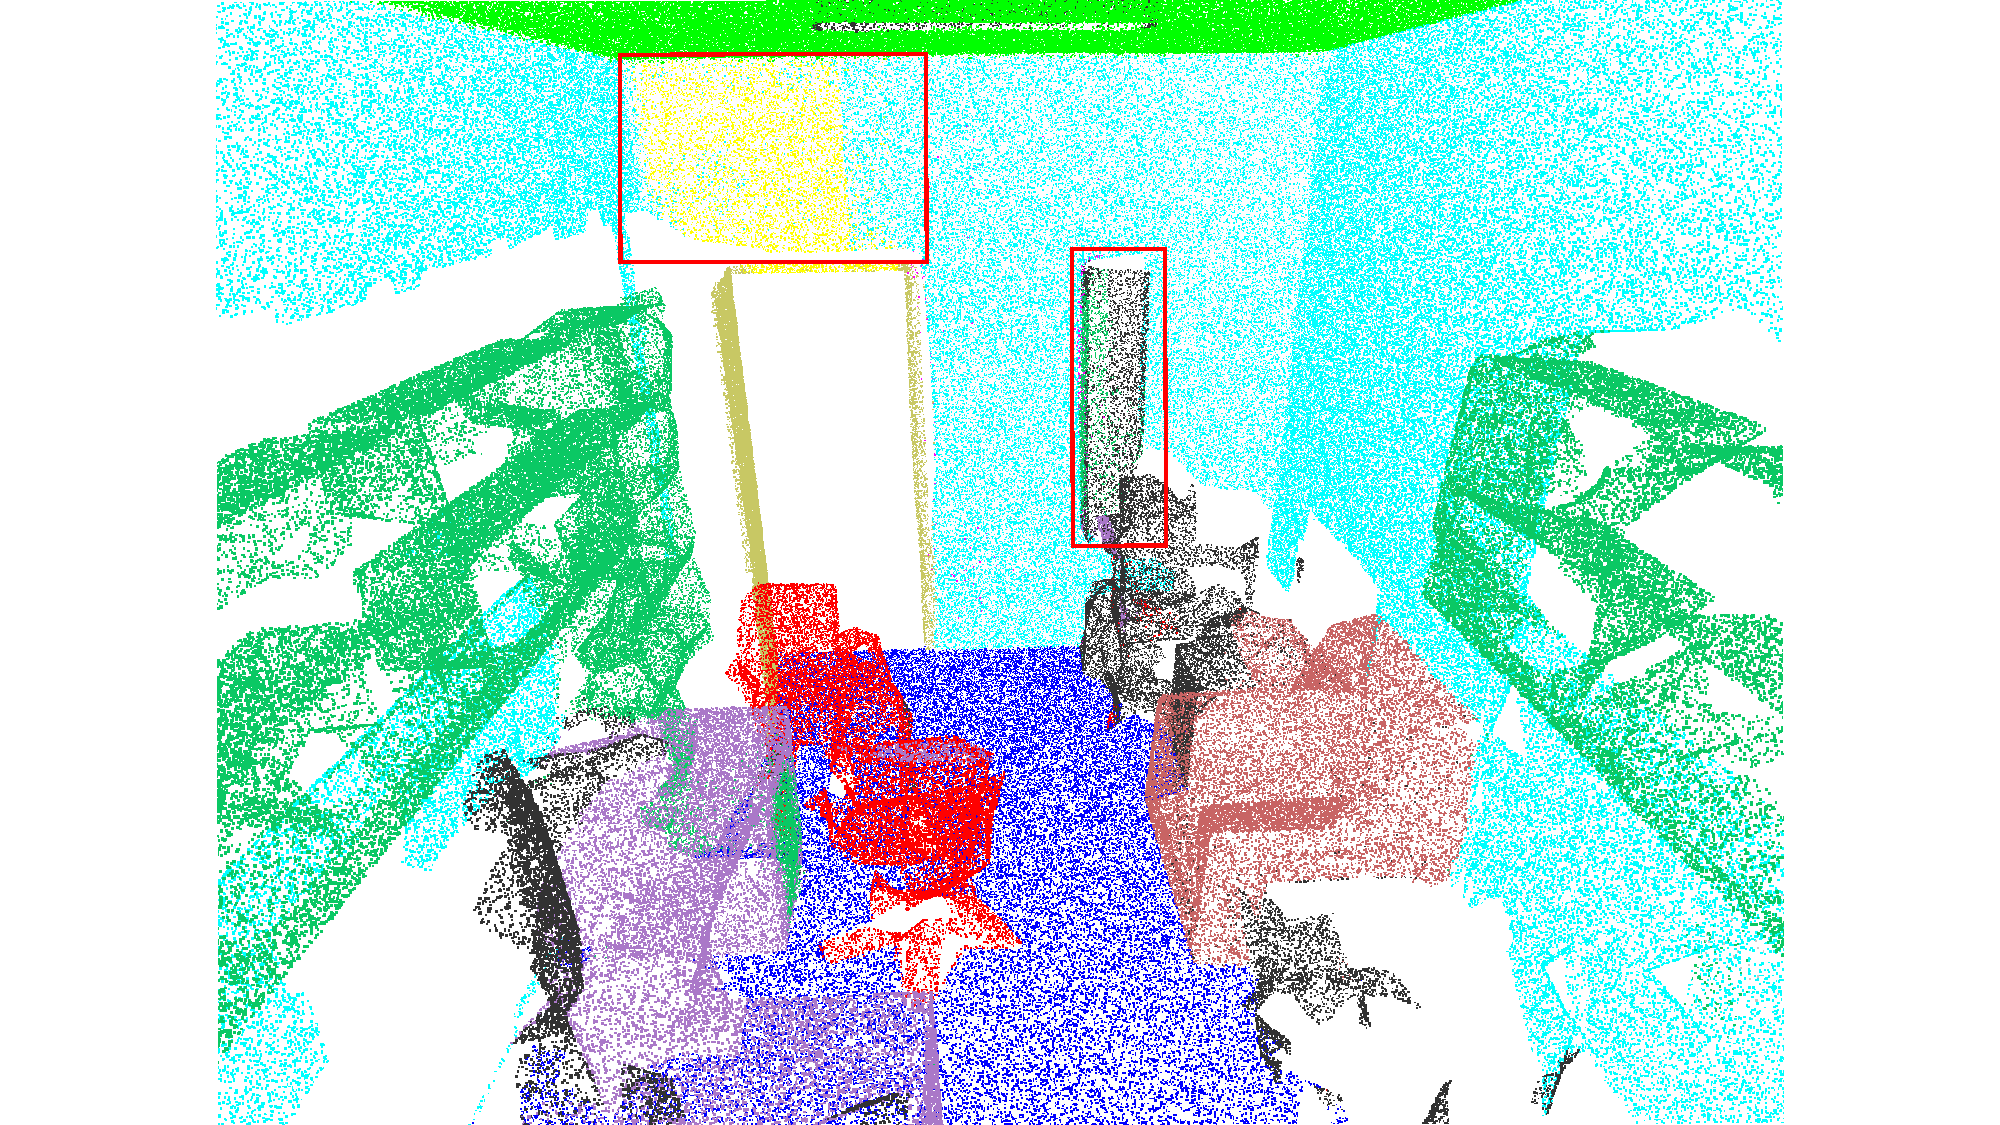
\includegraphics[width=\textwidth]{fig/supplement/semantic_segmentation/office_9/IDPT_office_9.pdf}
    \end{minipage}
    \hfill
    \begin{minipage}{0.22\textwidth}
        \centering
        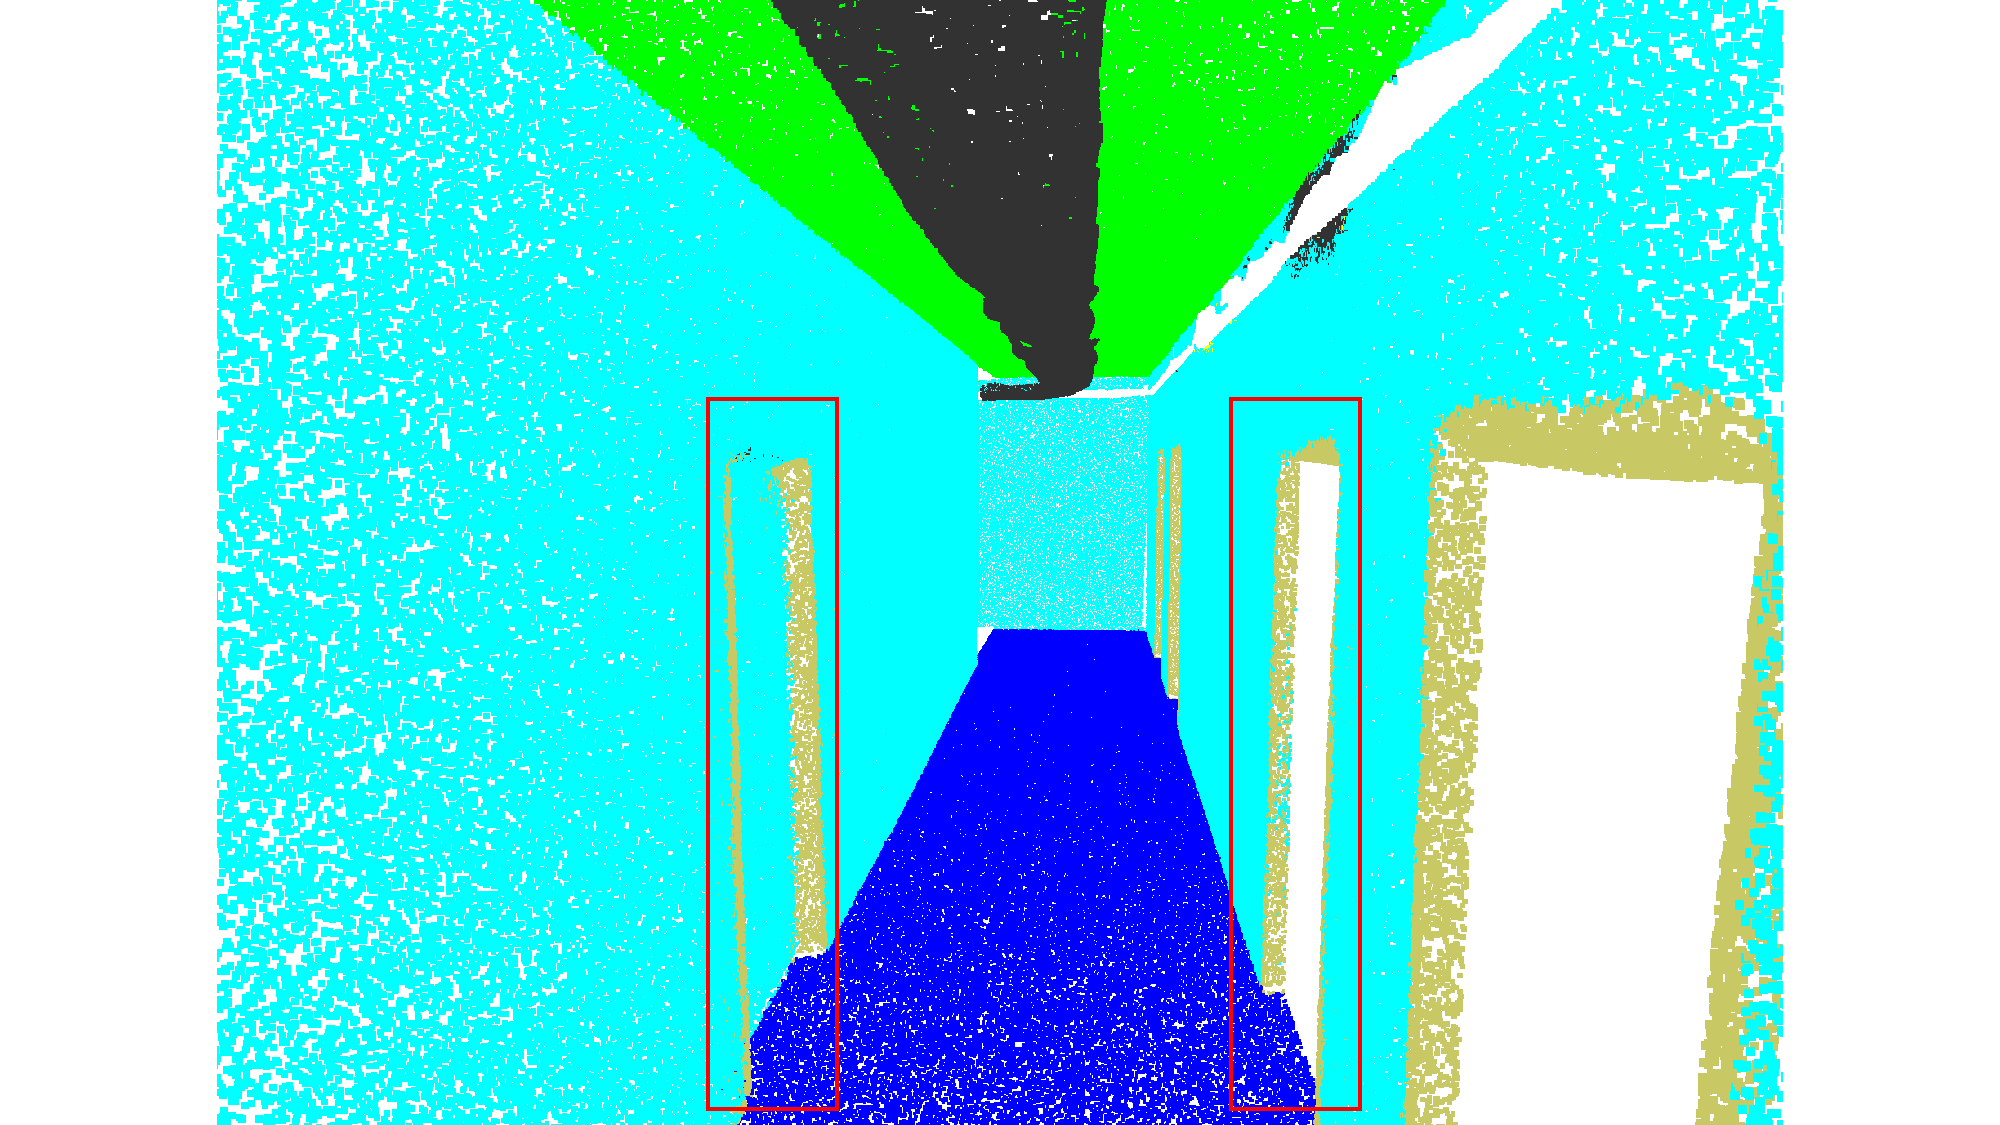
\includegraphics[width=\textwidth]{fig/supplement/semantic_segmentation/hallway_10/IDPT_hallway_10.pdf}
    \end{minipage}
    \hfill
    \begin{minipage}{0.22\textwidth}
        \centering
        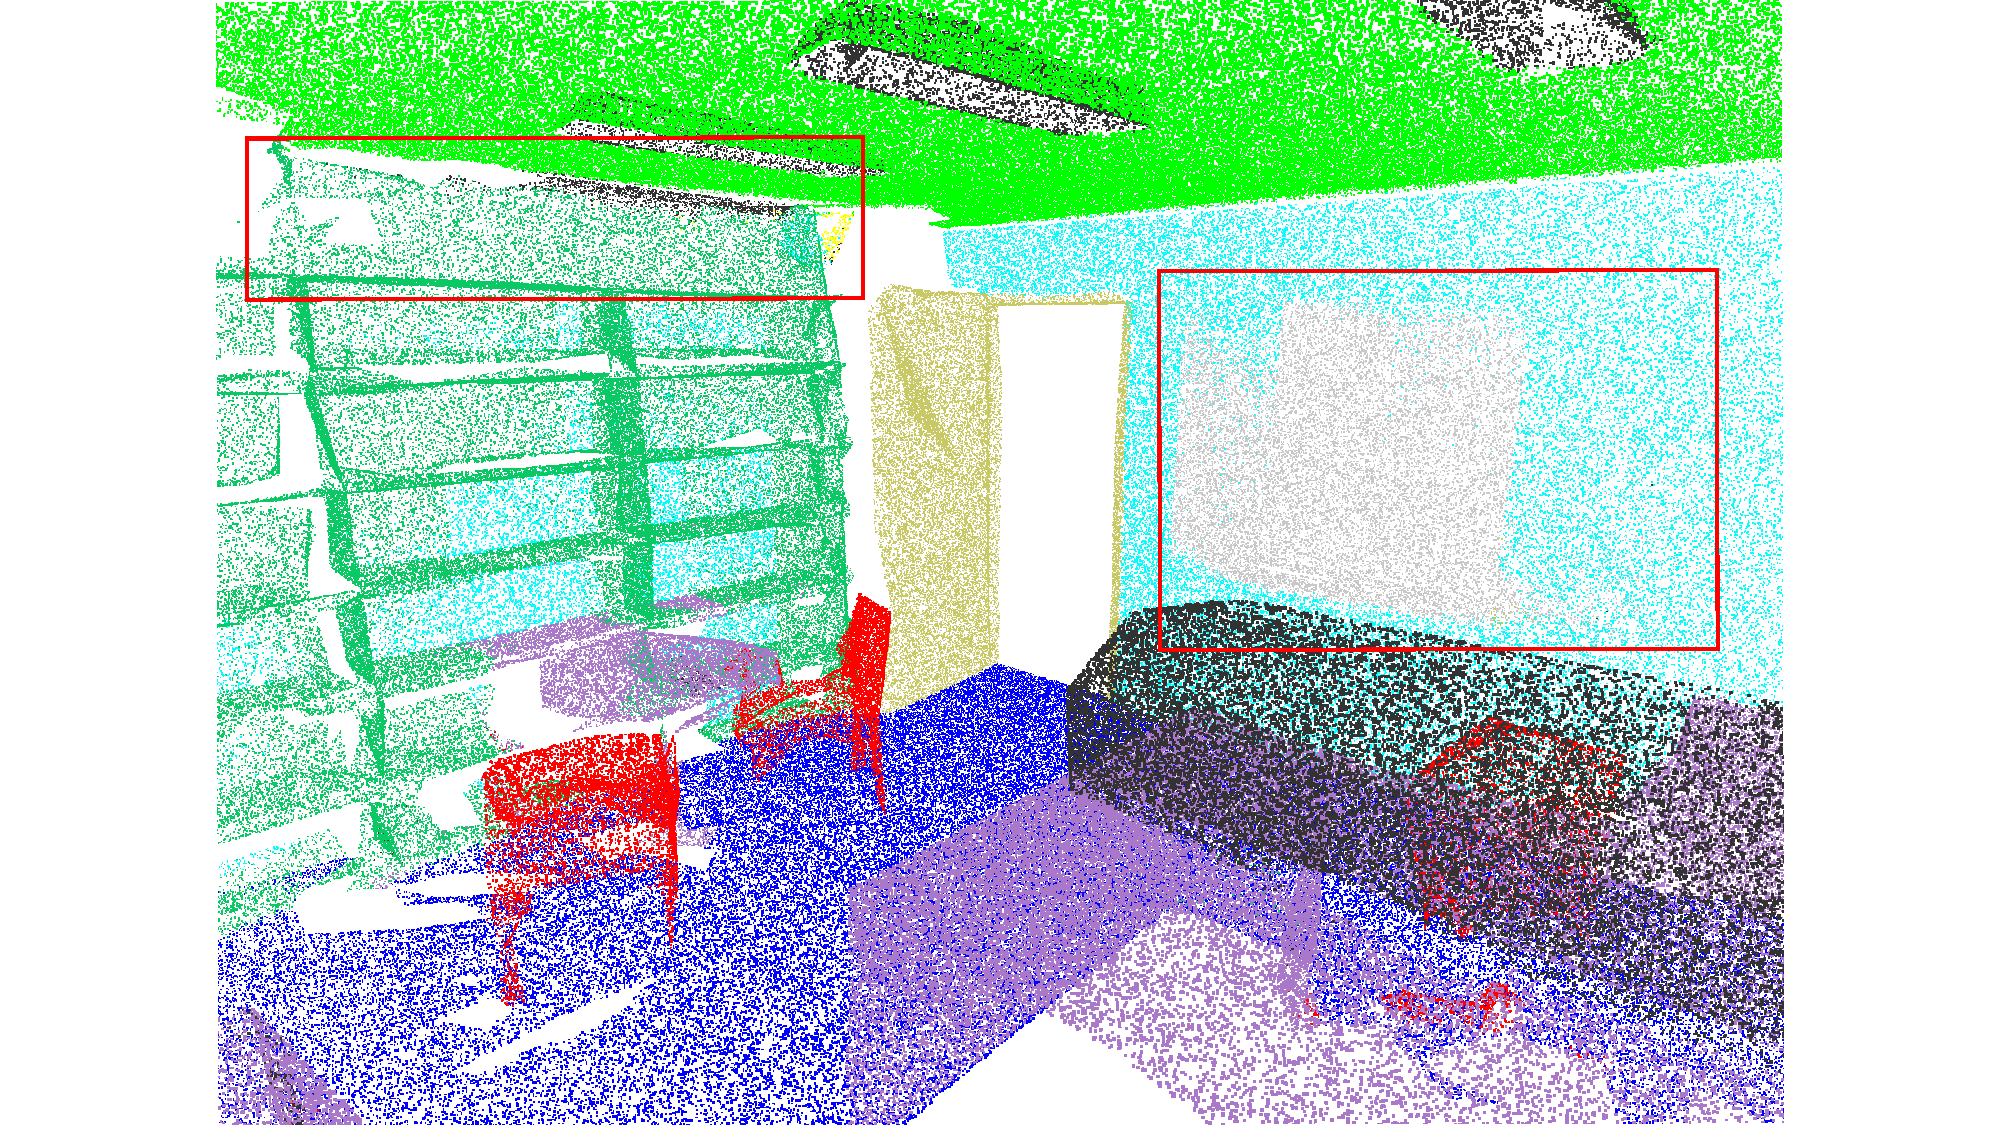
\includegraphics[width=\textwidth]{fig/supplement/semantic_segmentation/office_35/IDPT_office_35.pdf}
    \end{minipage}
    \hfill
    \begin{minipage}{0.22\textwidth}
        \centering
        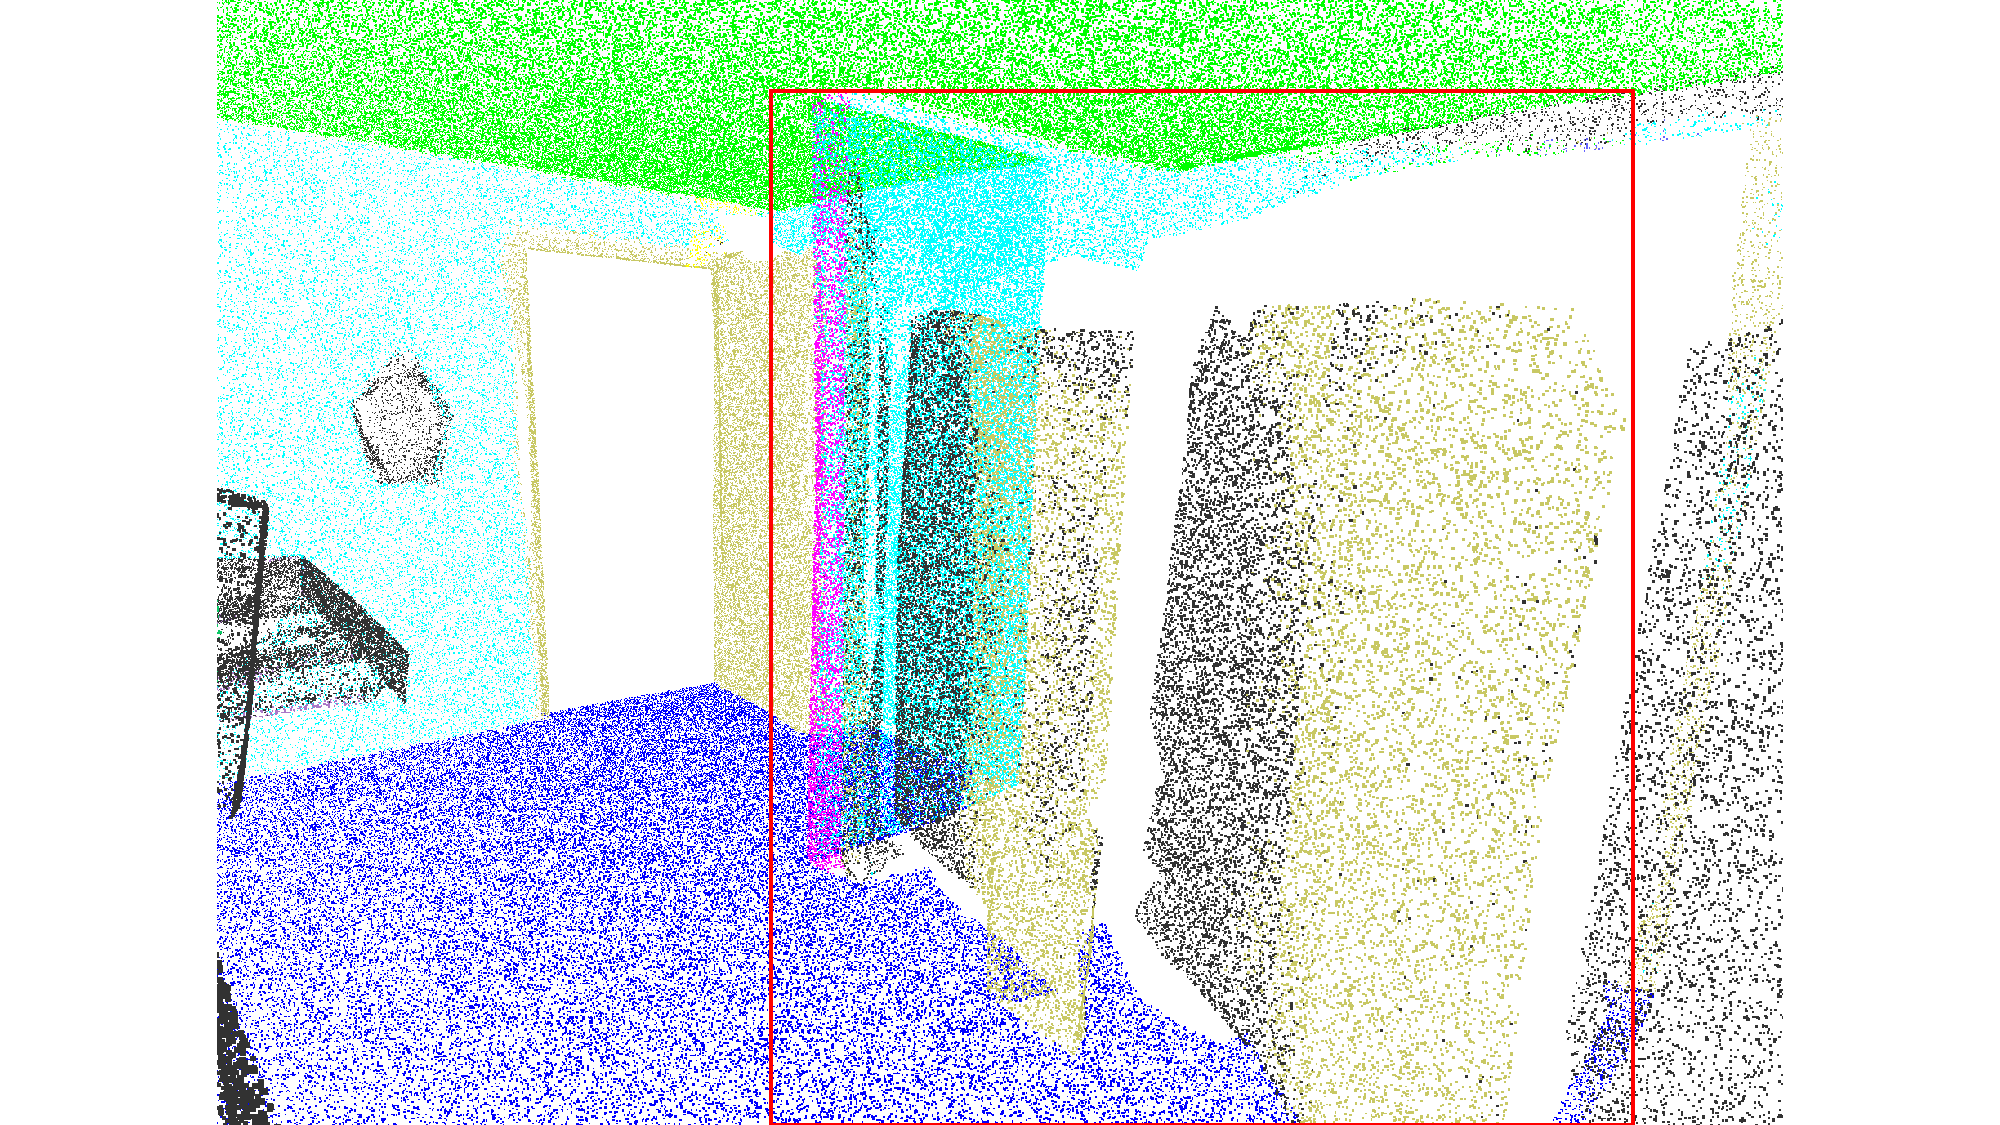
\includegraphics[width=\textwidth]{fig/supplement/semantic_segmentation/wc_2/IDPT_wc_2.pdf}
    \end{minipage}
    \hfill

    % 换行
    \vspace{0.5em}

    % 第四行左侧的竖排标签
    \begin{minipage}{0.09\textwidth}
        \centering
        PPT
    \end{minipage}
    \hfill
    % 第四行图片
    \begin{minipage}{0.22\textwidth}
        \centering
        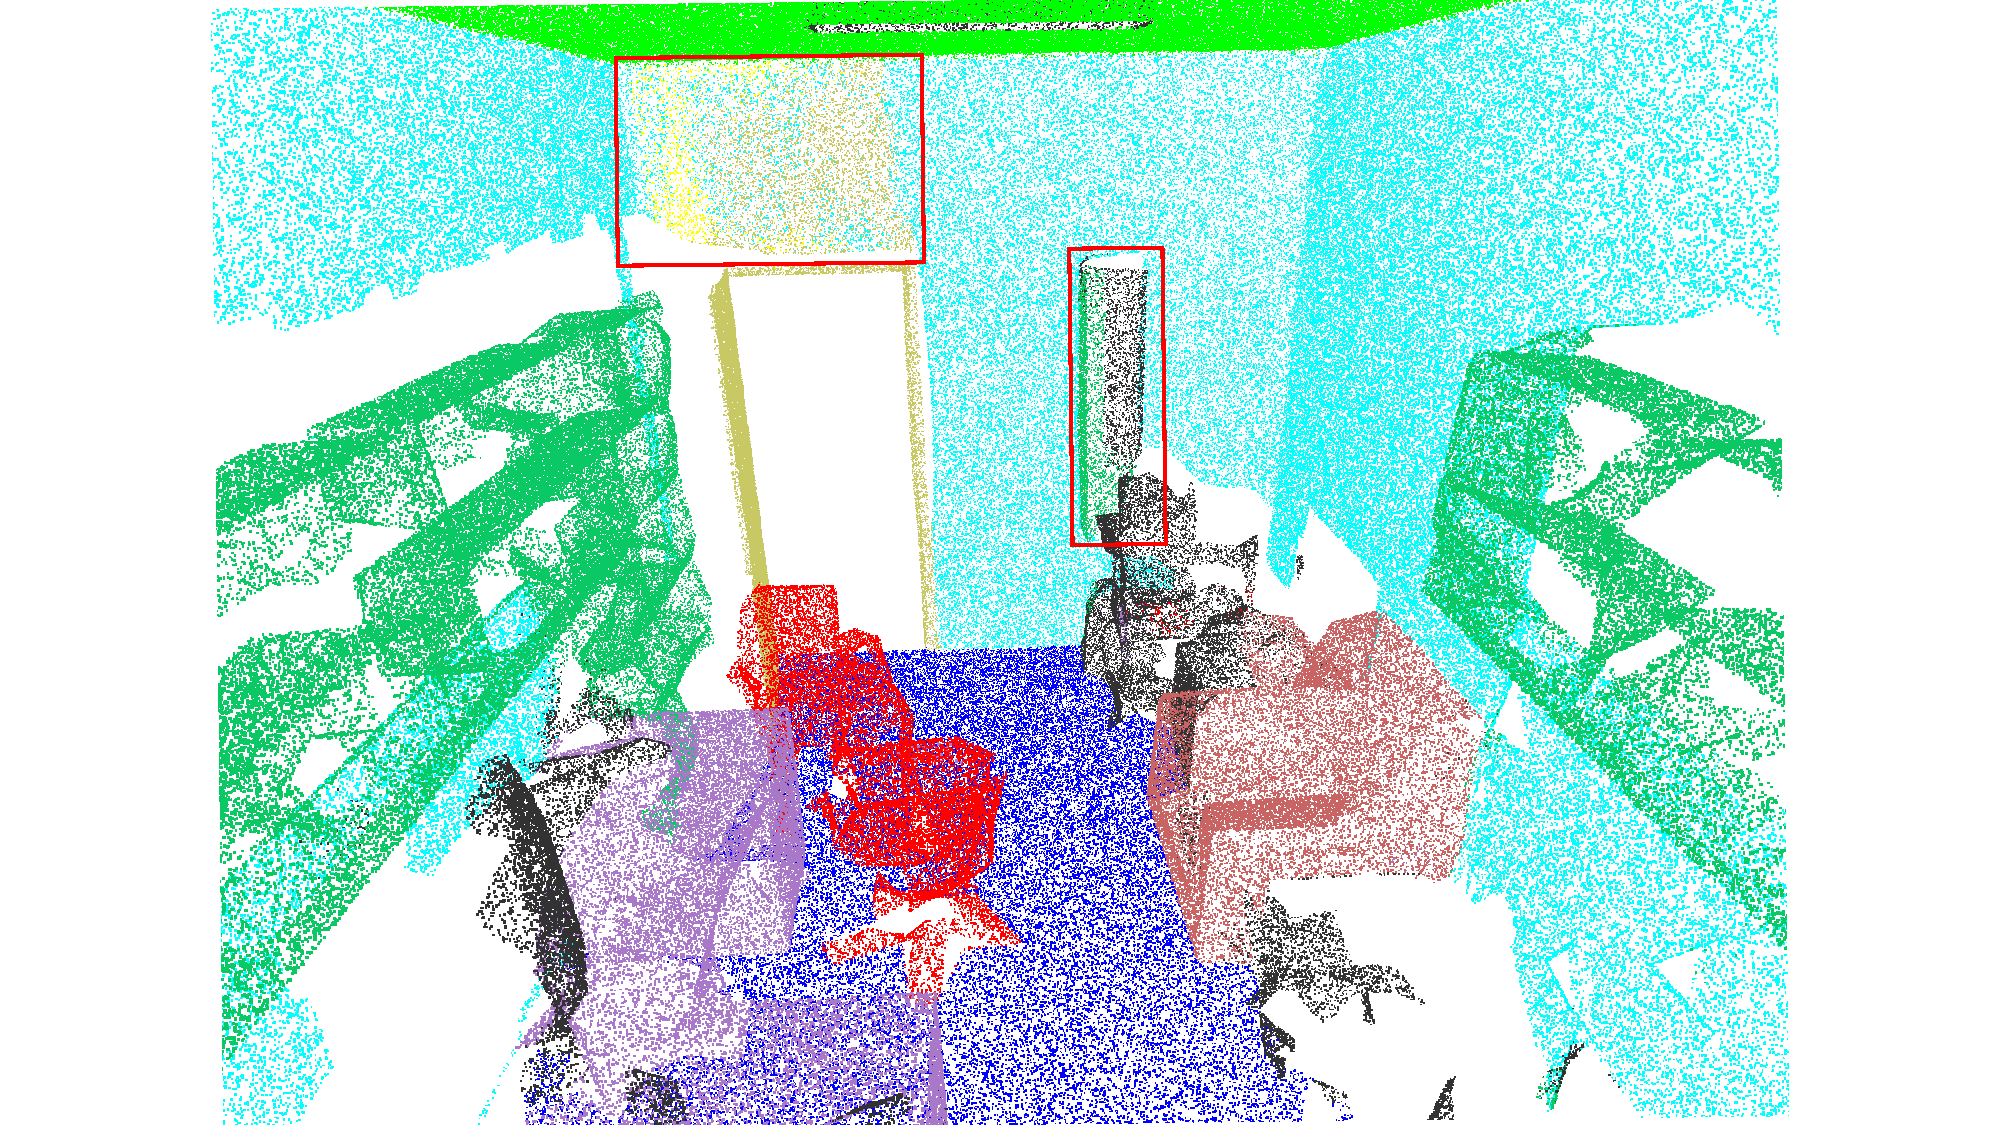
\includegraphics[width=\textwidth]{fig/supplement/semantic_segmentation/office_9/PPT_office_9.pdf}
    \end{minipage}
    \hfill
     \begin{minipage}{0.22\textwidth}
        \centering
        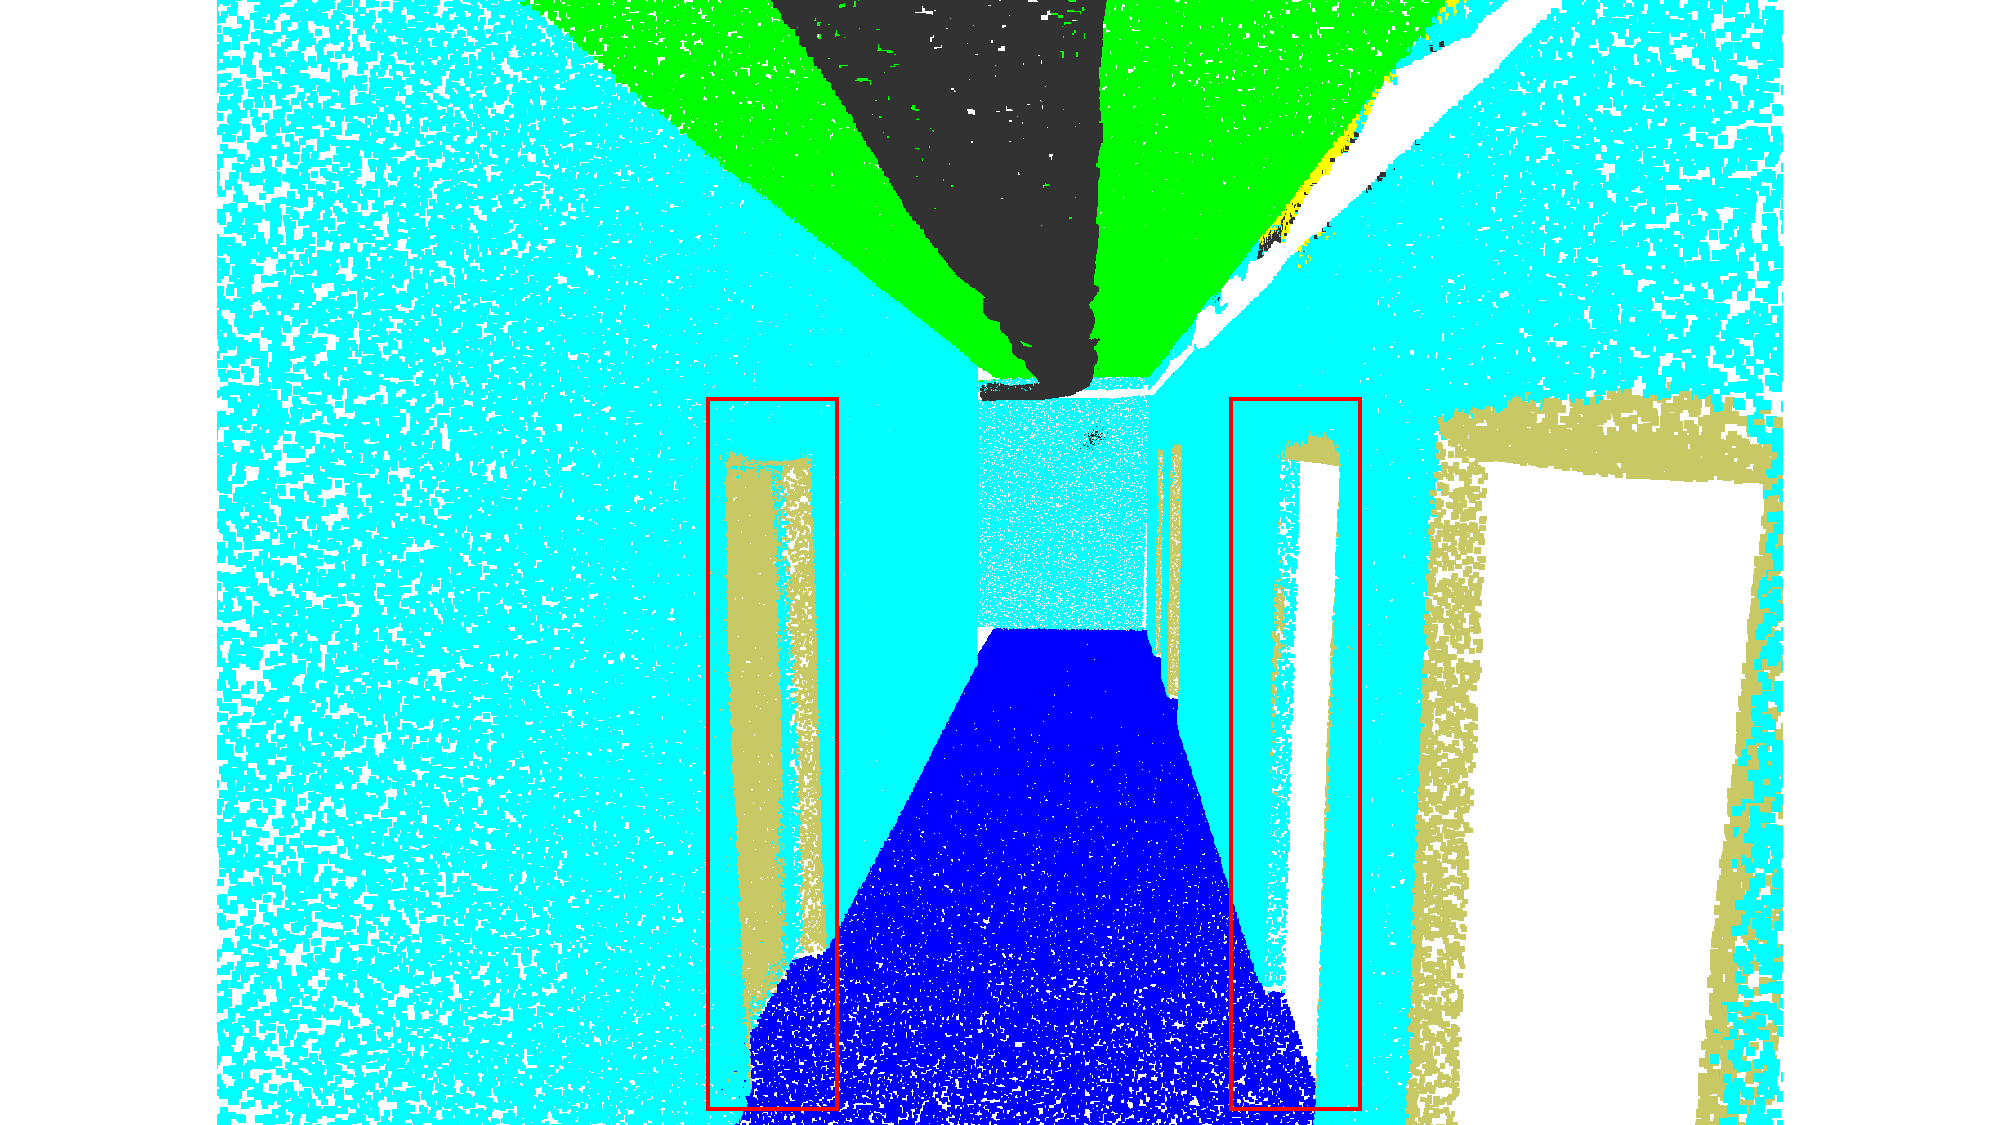
\includegraphics[width=\textwidth]{fig/supplement/semantic_segmentation/hallway_10/PPT_hallway_10.pdf}
    \end{minipage}
    \hfill
    \begin{minipage}{0.22\textwidth}
        \centering
        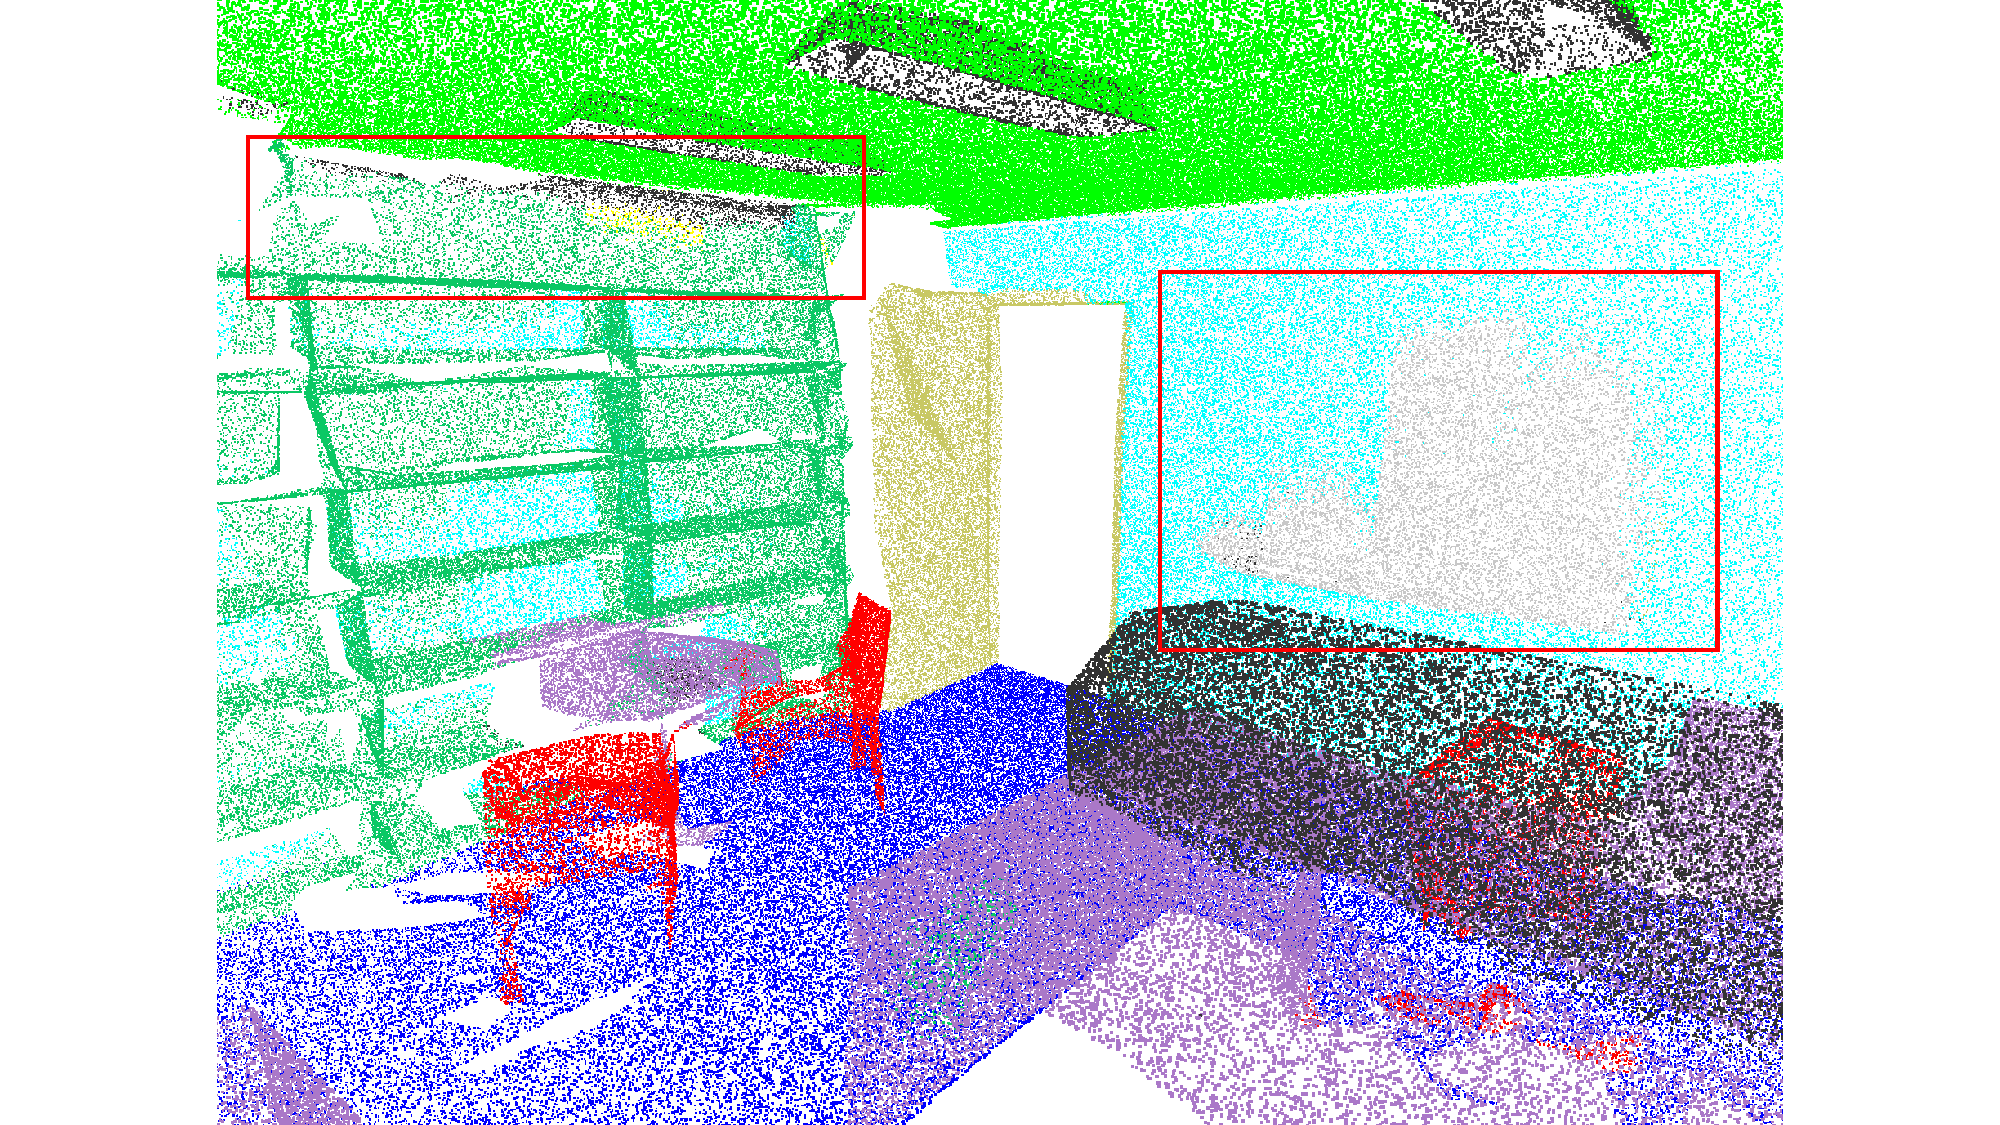
\includegraphics[width=\textwidth]{fig/supplement/semantic_segmentation/office_35/PPT_office_35.pdf}
    \end{minipage}
    \hfill
    \begin{minipage}{0.22\textwidth}
        \centering
        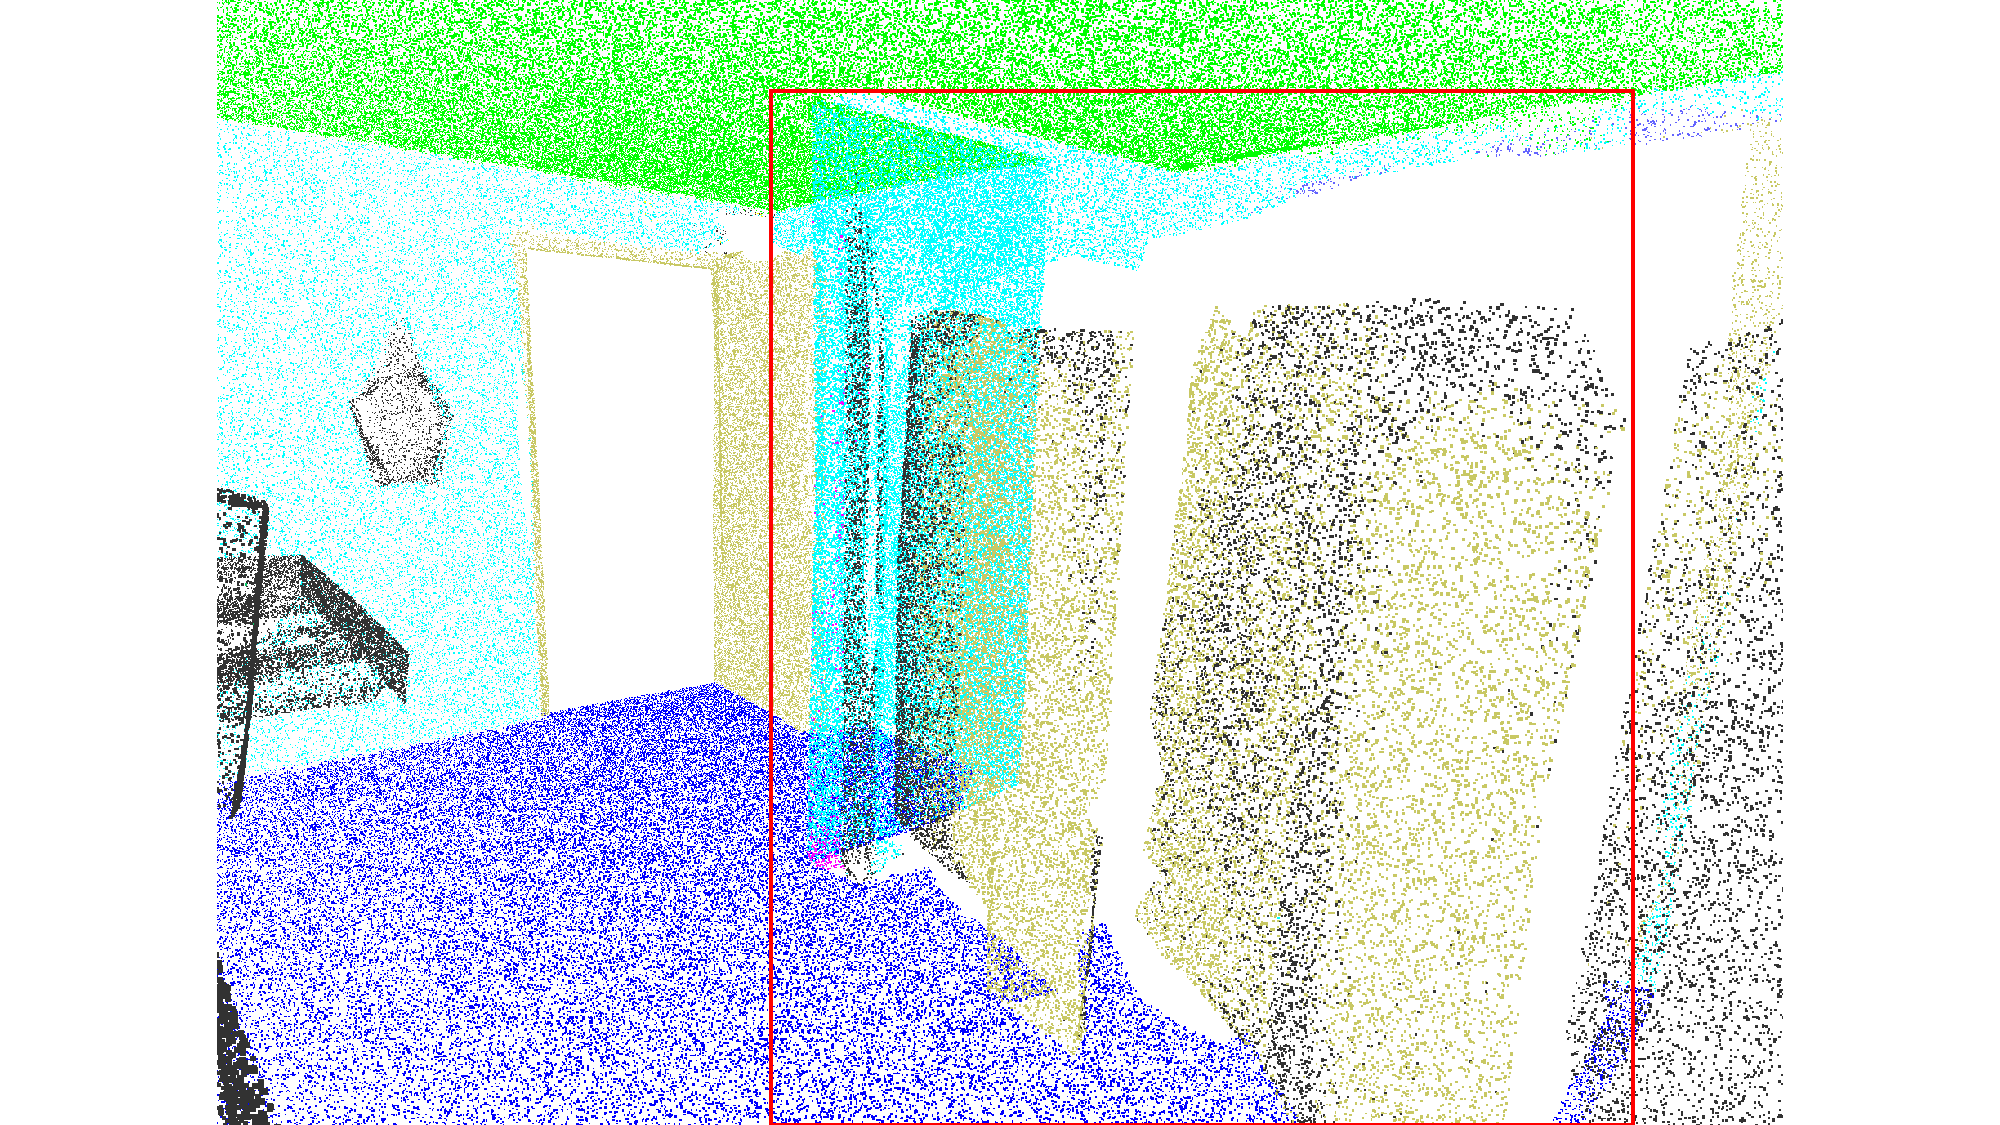
\includegraphics[width=\textwidth]{fig/supplement/semantic_segmentation/wc_2/PPT_wc_2.pdf}
    \end{minipage}
    \hfill

    % 换行
    \vspace{0.5em}

    % 第五行左侧的竖排标签
    \begin{minipage}{0.09\textwidth}
        \centering
        PointGST
    \end{minipage}
    \hfill
    % 第五行图片
    \begin{minipage}{0.22\textwidth}
        \centering
        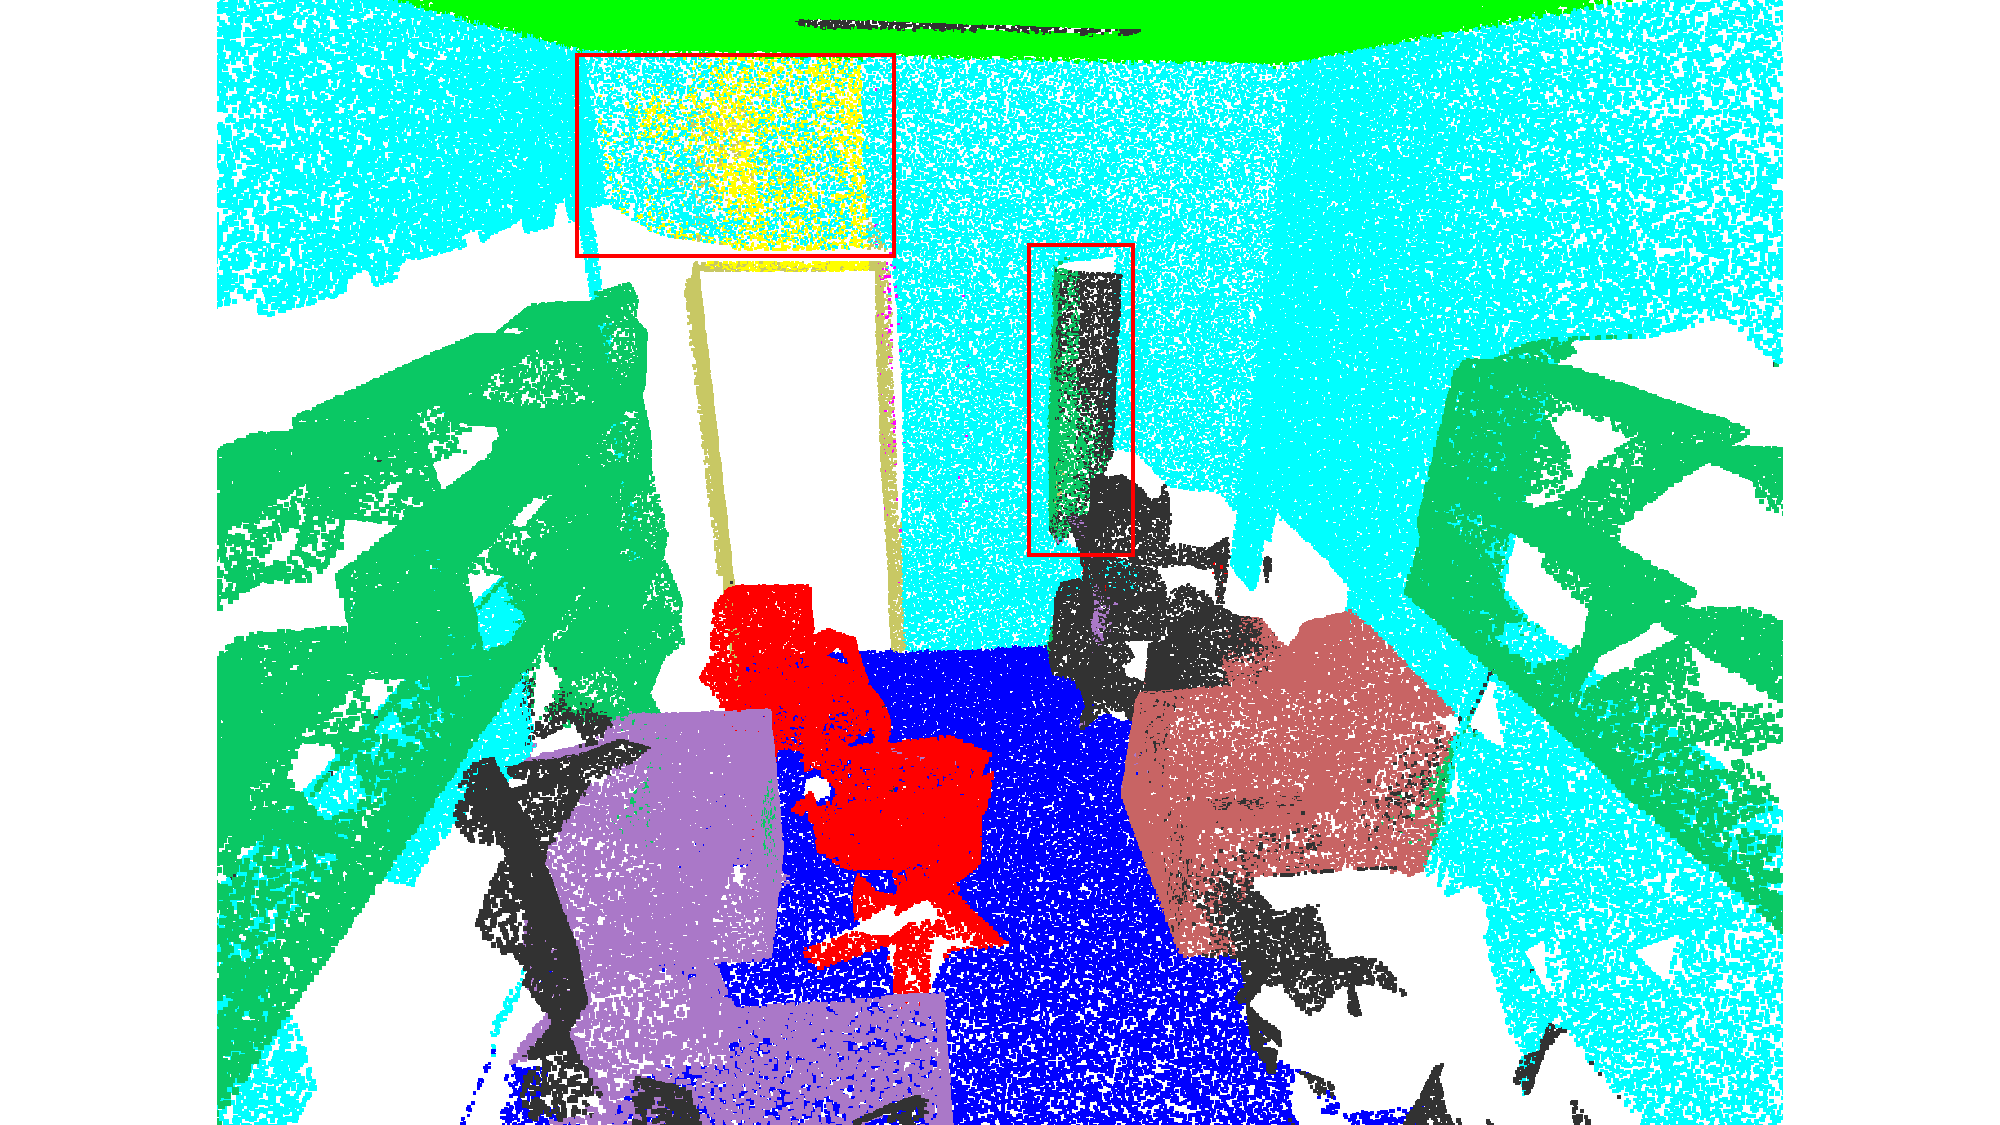
\includegraphics[width=\textwidth]{fig/supplement/semantic_segmentation/office_9/PointGST_office_9.pdf}
    \end{minipage}
    \hfill
    \begin{minipage}{0.22\textwidth}
        \centering
        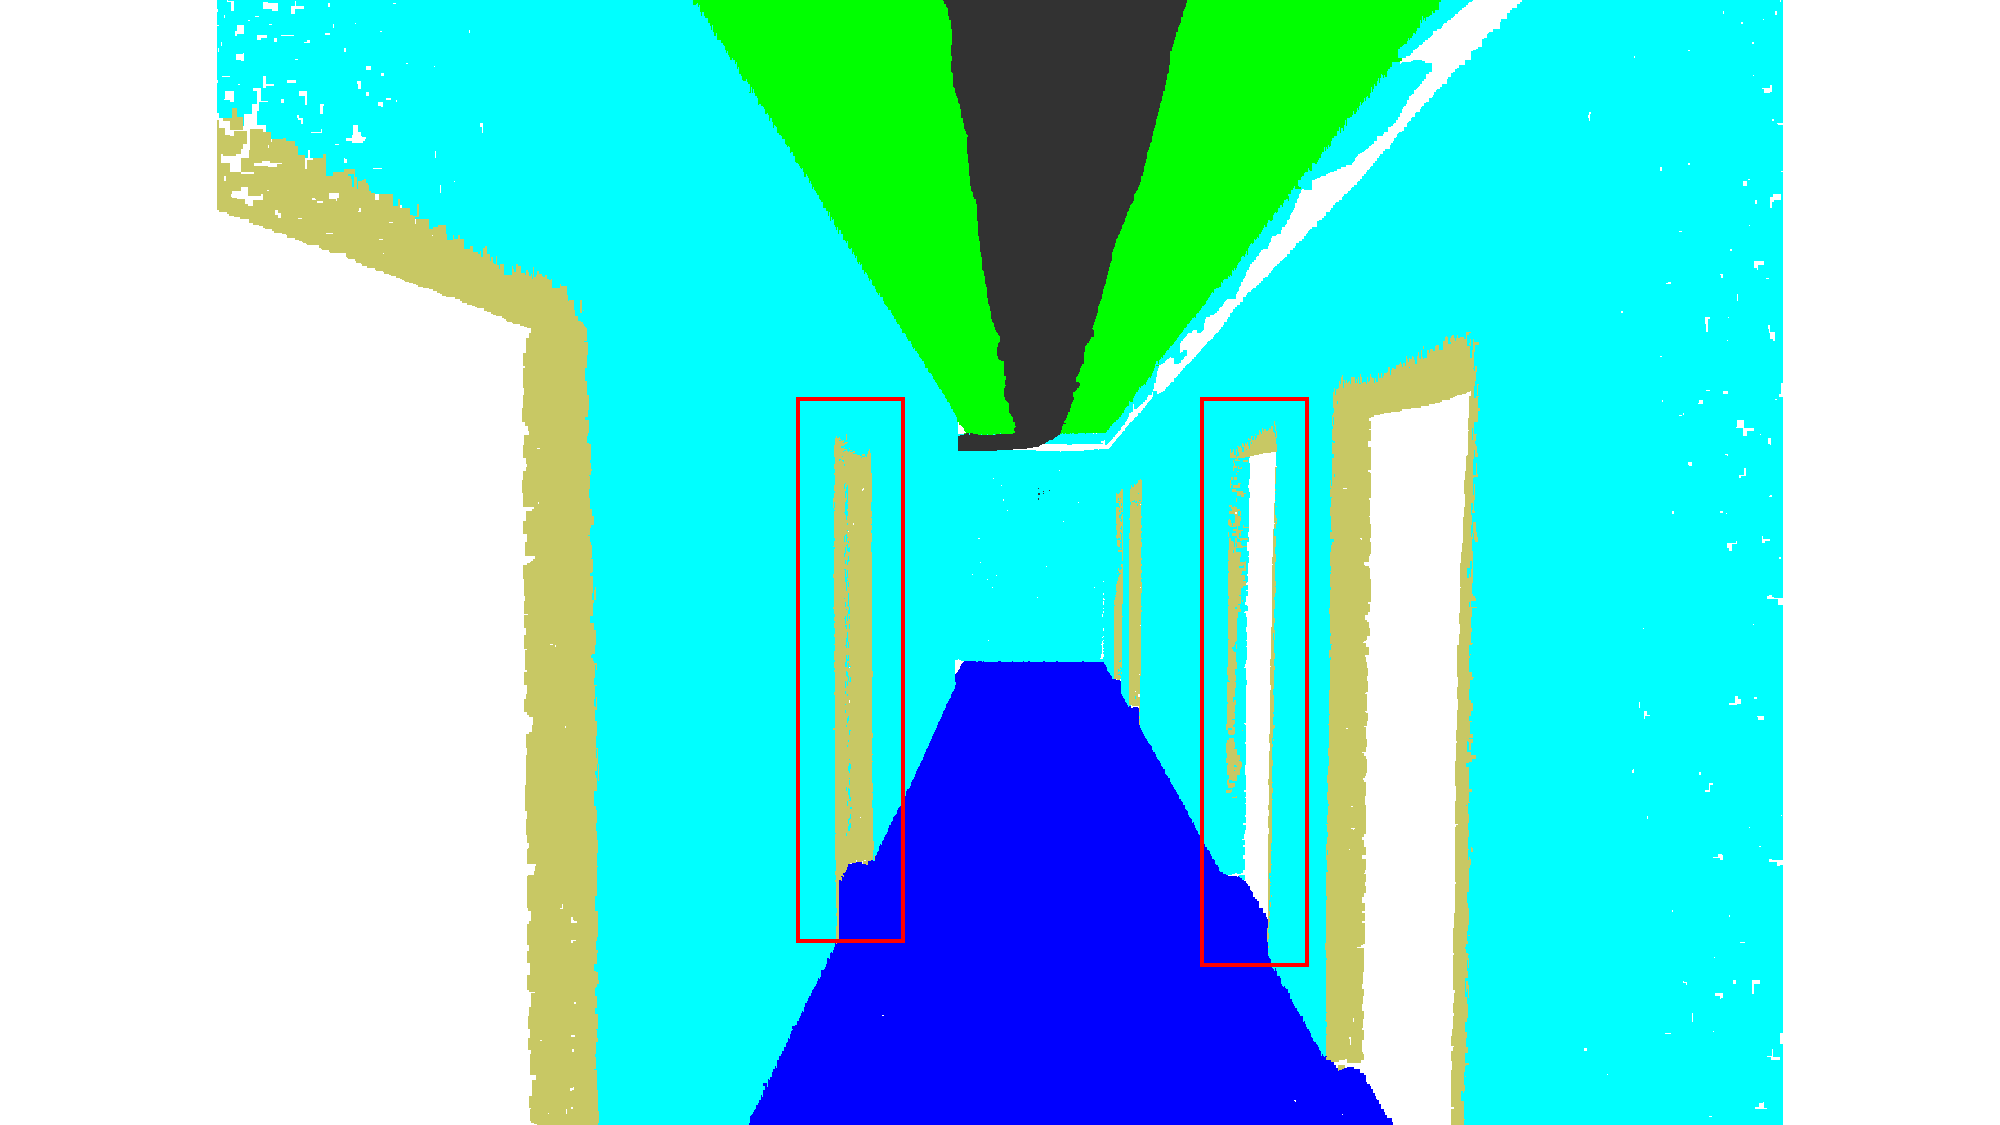
\includegraphics[width=\textwidth]{fig/supplement/semantic_segmentation/hallway_10/PointGST_hallway_10.pdf}
    \end{minipage}
    \hfill
    \begin{minipage}{0.22\textwidth}
        \centering
        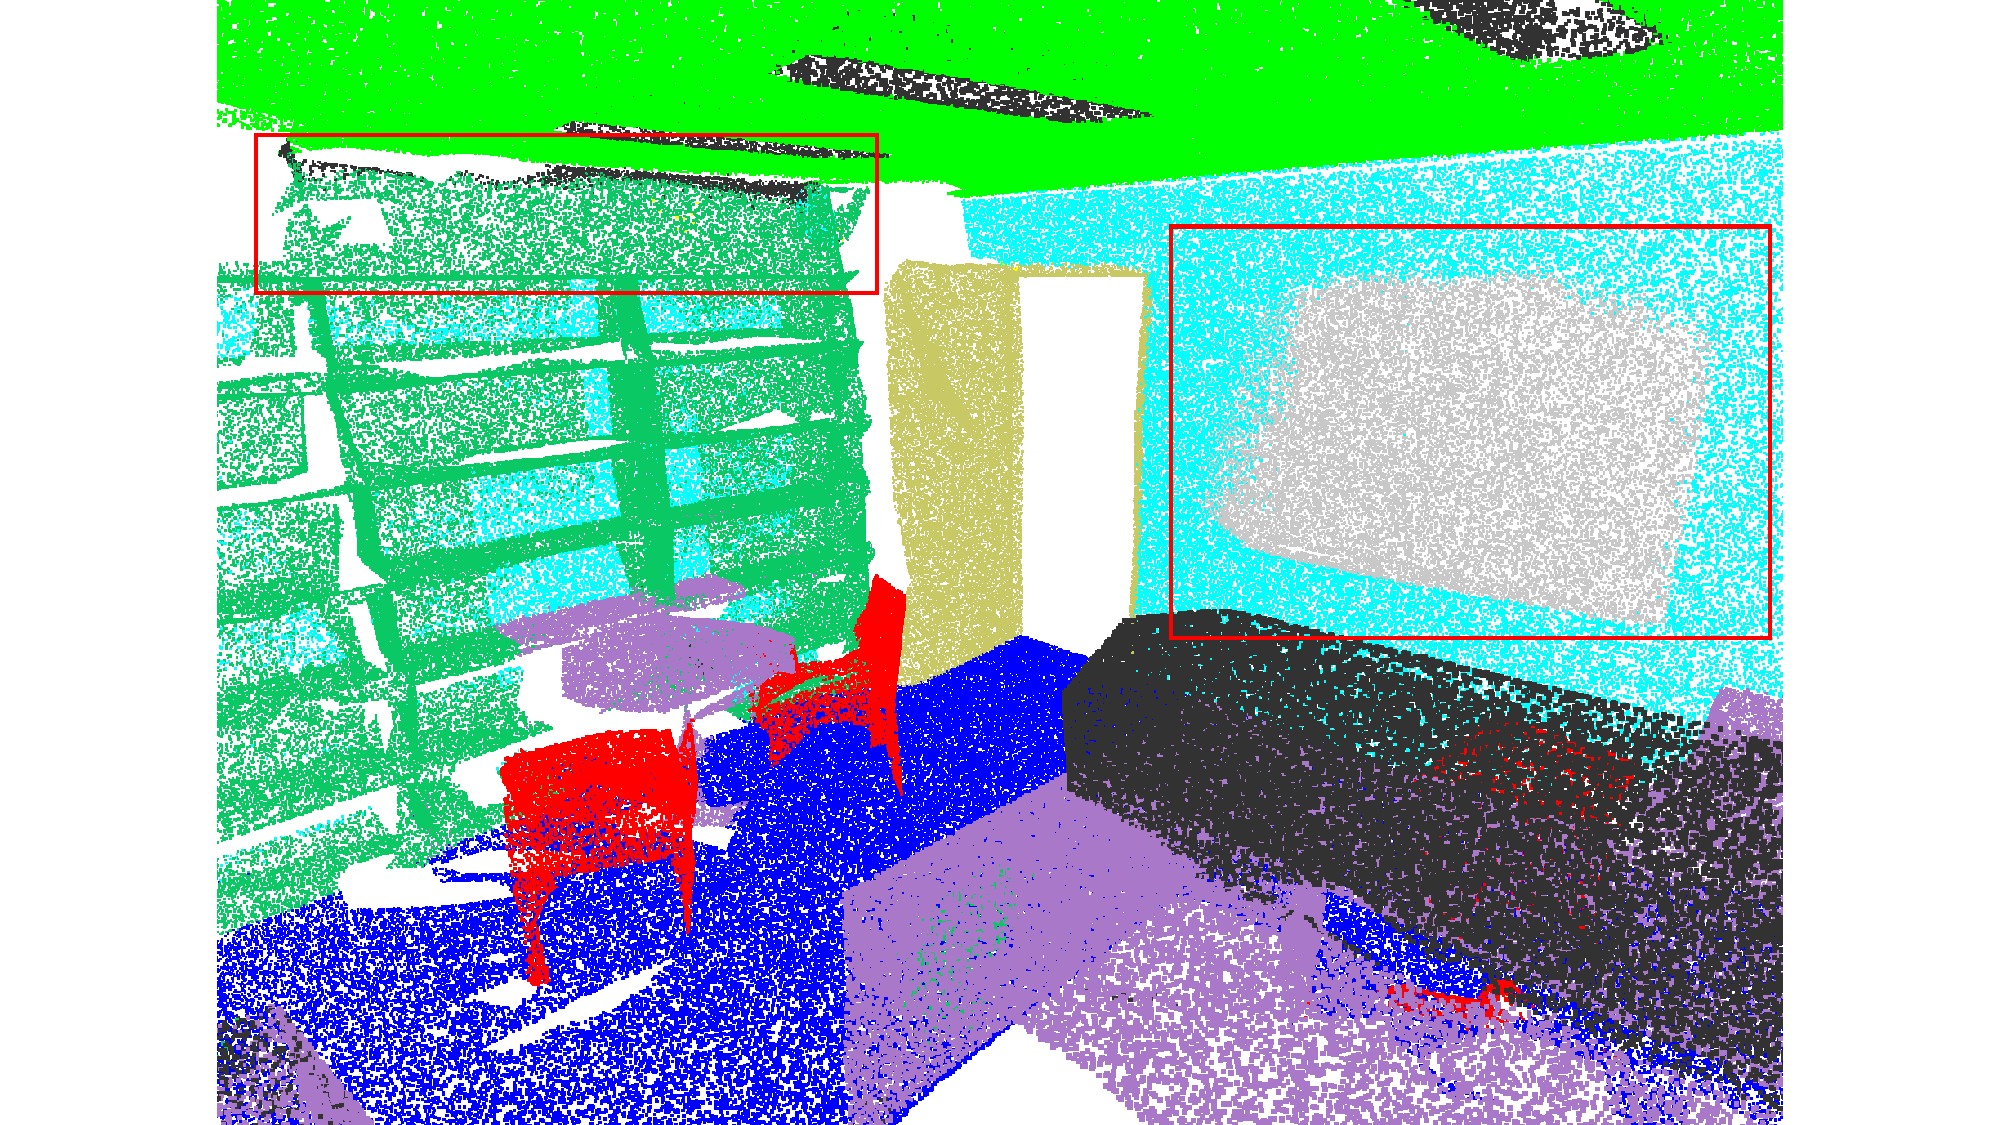
\includegraphics[width=\textwidth]{fig/supplement/semantic_segmentation/office_35/PointGST_office_35.pdf}
    \end{minipage}
    \hfill
    \begin{minipage}{0.22\textwidth}
        \centering
        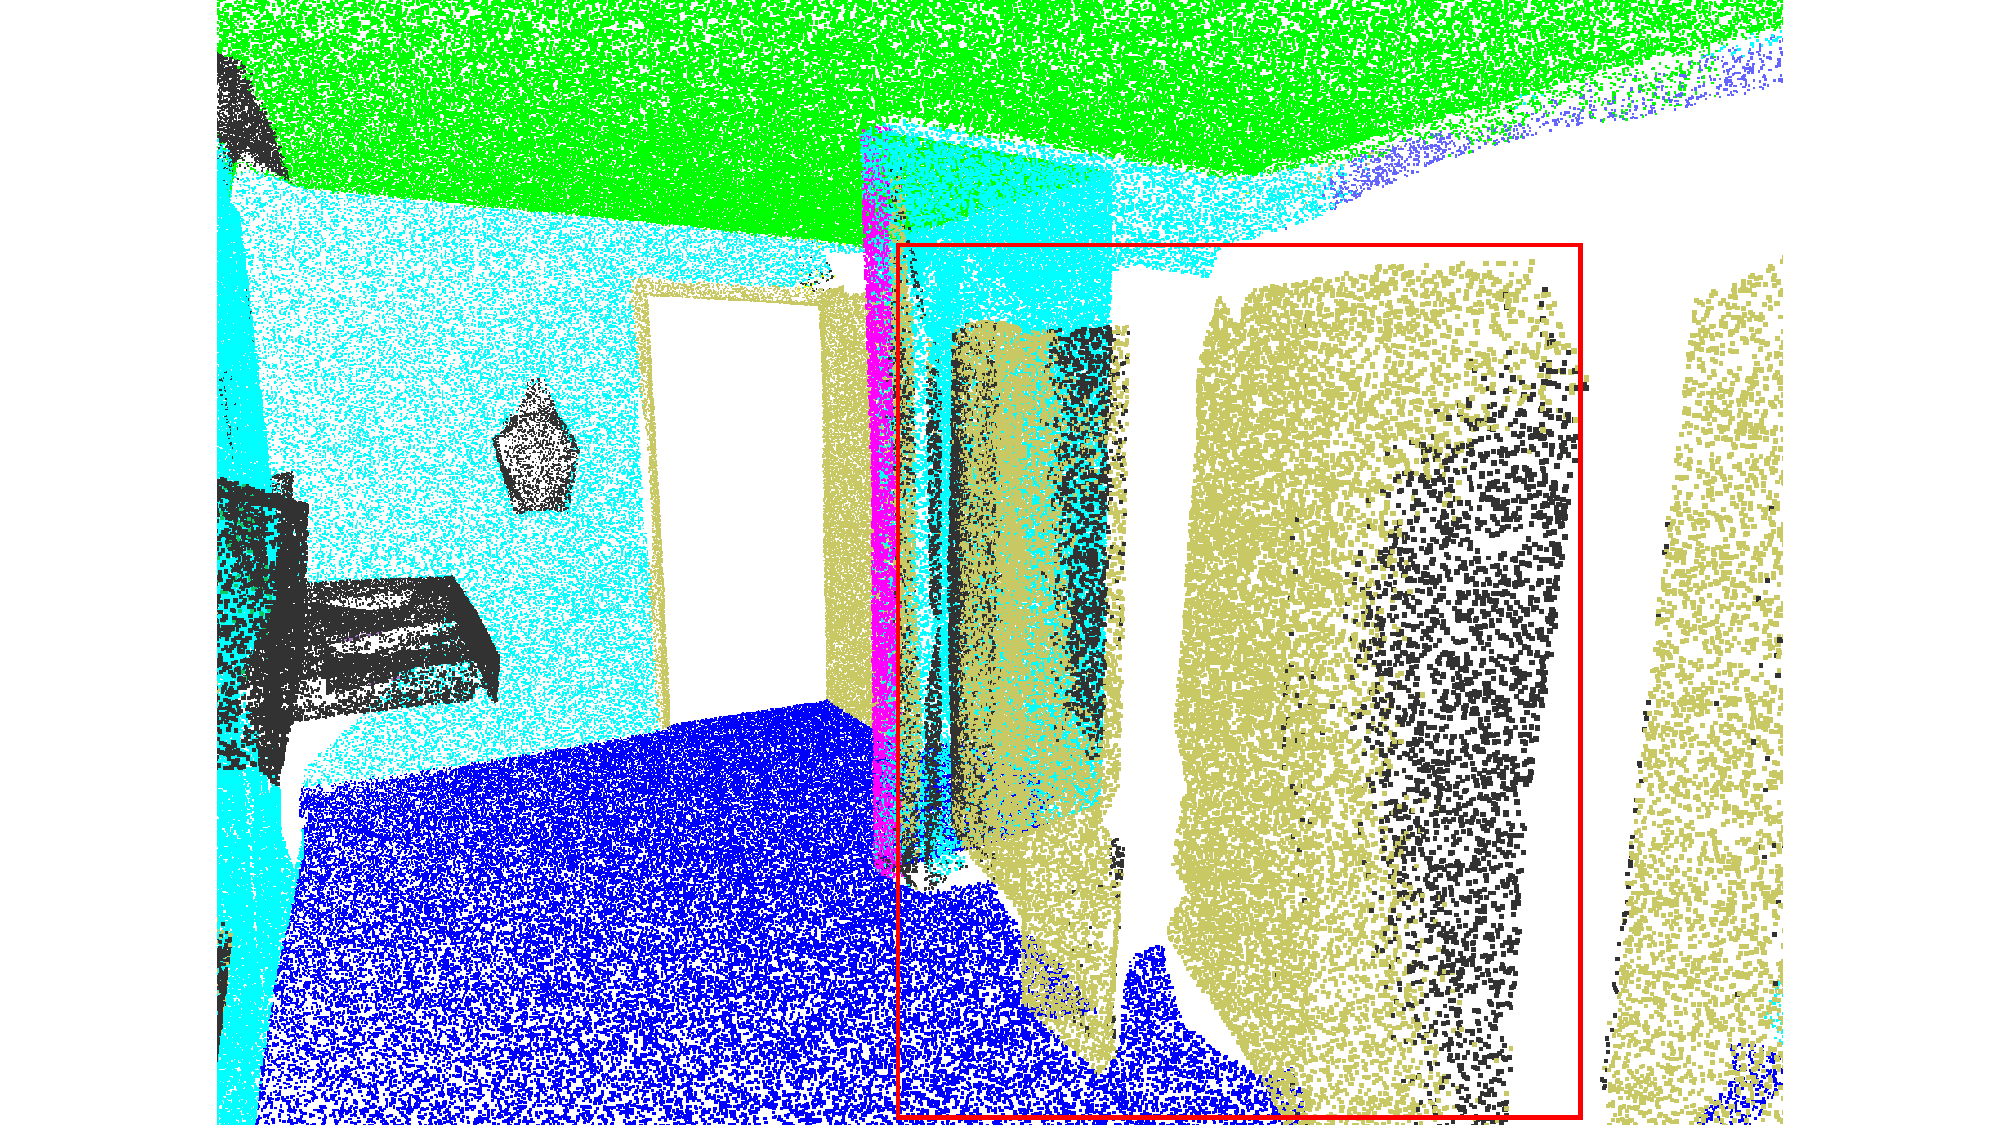
\includegraphics[width=\textwidth]{fig/supplement/semantic_segmentation/wc_2/PointGST_wc_2.pdf}
    \end{minipage}
    \hfill

    % 换行
    \vspace{0.5em}

    % 第六行左侧的竖排标签
    \begin{minipage}{0.09\textwidth}
        \centering
        PLT (Ours)
    \end{minipage}
    \hfill
    % 第六行图片
    \begin{minipage}{0.22\textwidth}
        \centering
        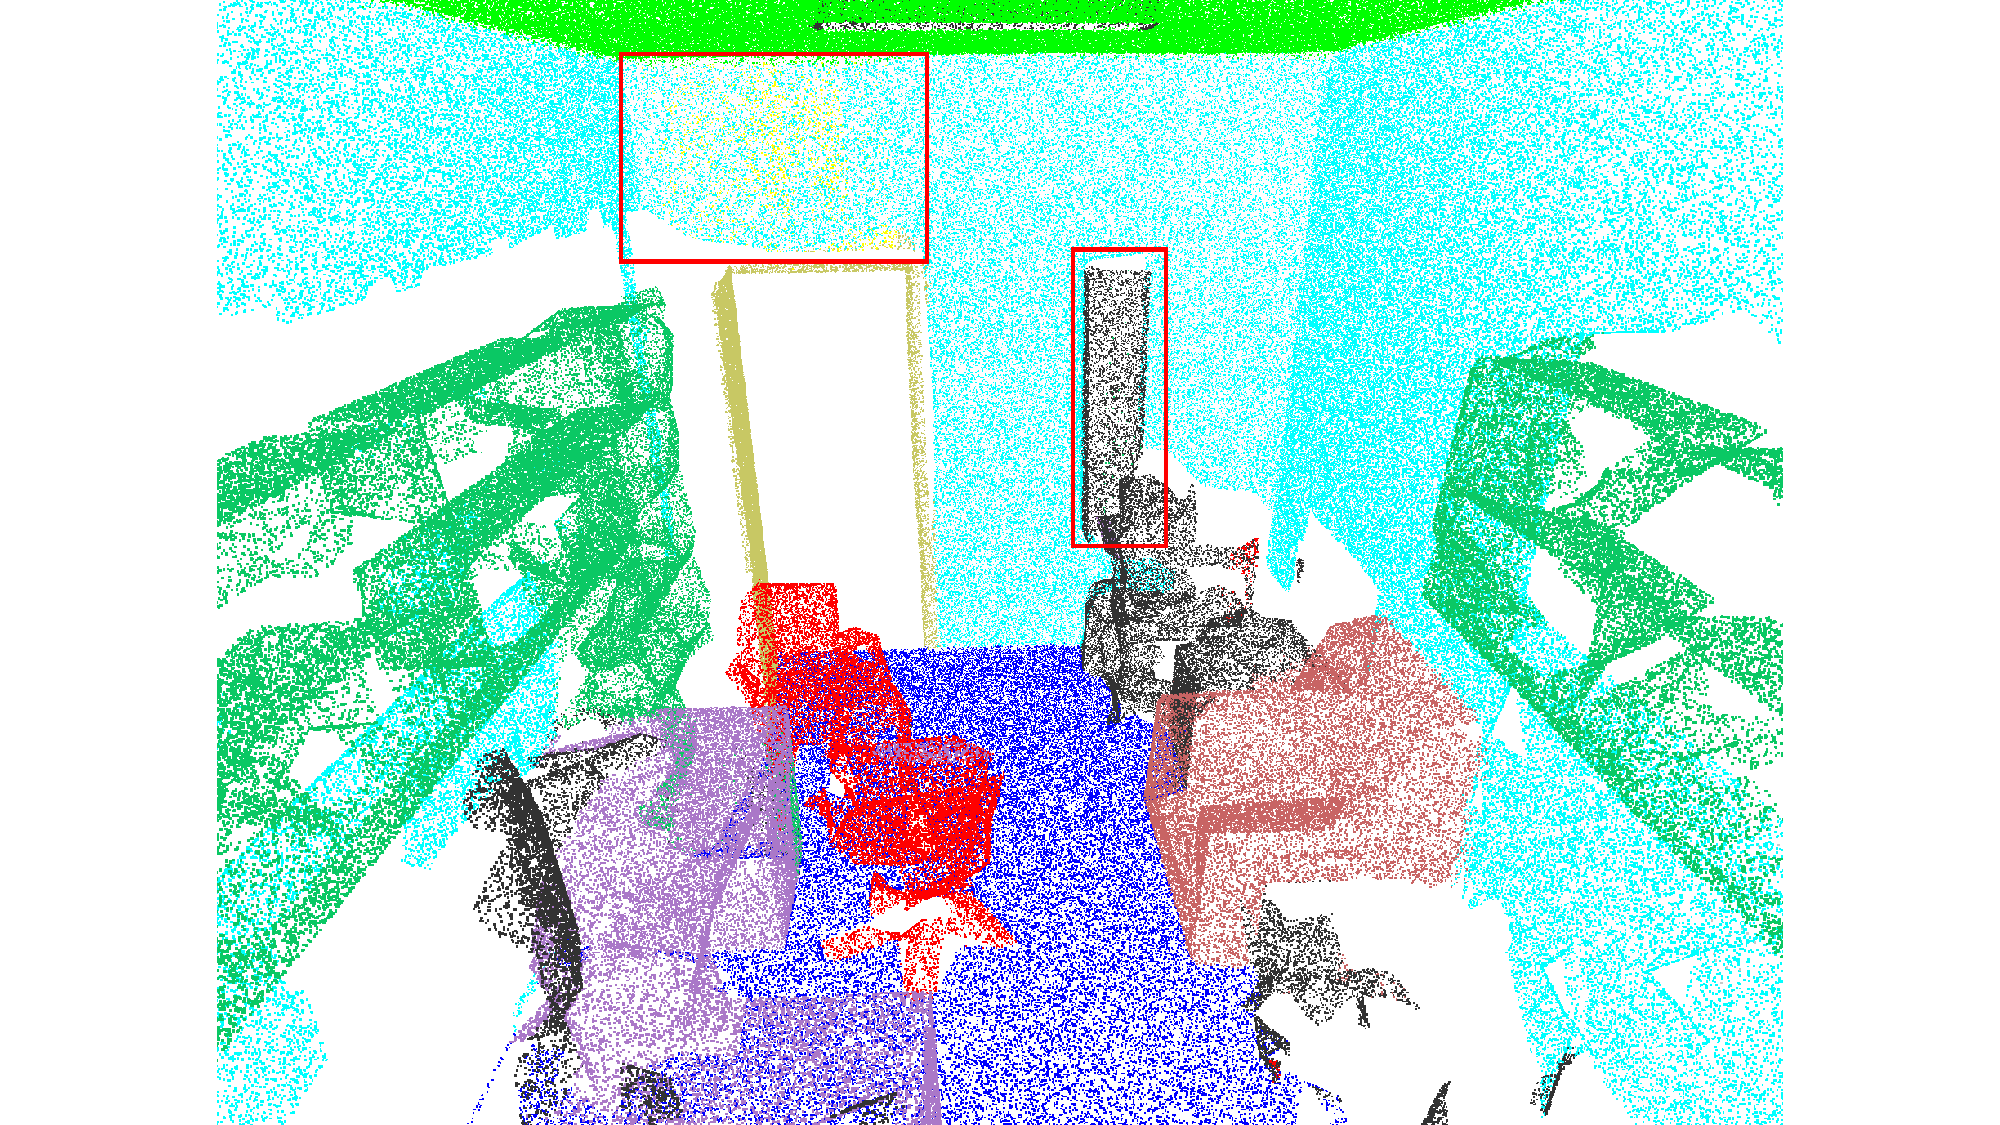
\includegraphics[width=\textwidth]{fig/supplement/semantic_segmentation/office_9/PLT_office_9.pdf}
    \end{minipage}
    \hfill
    \begin{minipage}{0.22\textwidth}
        \centering
        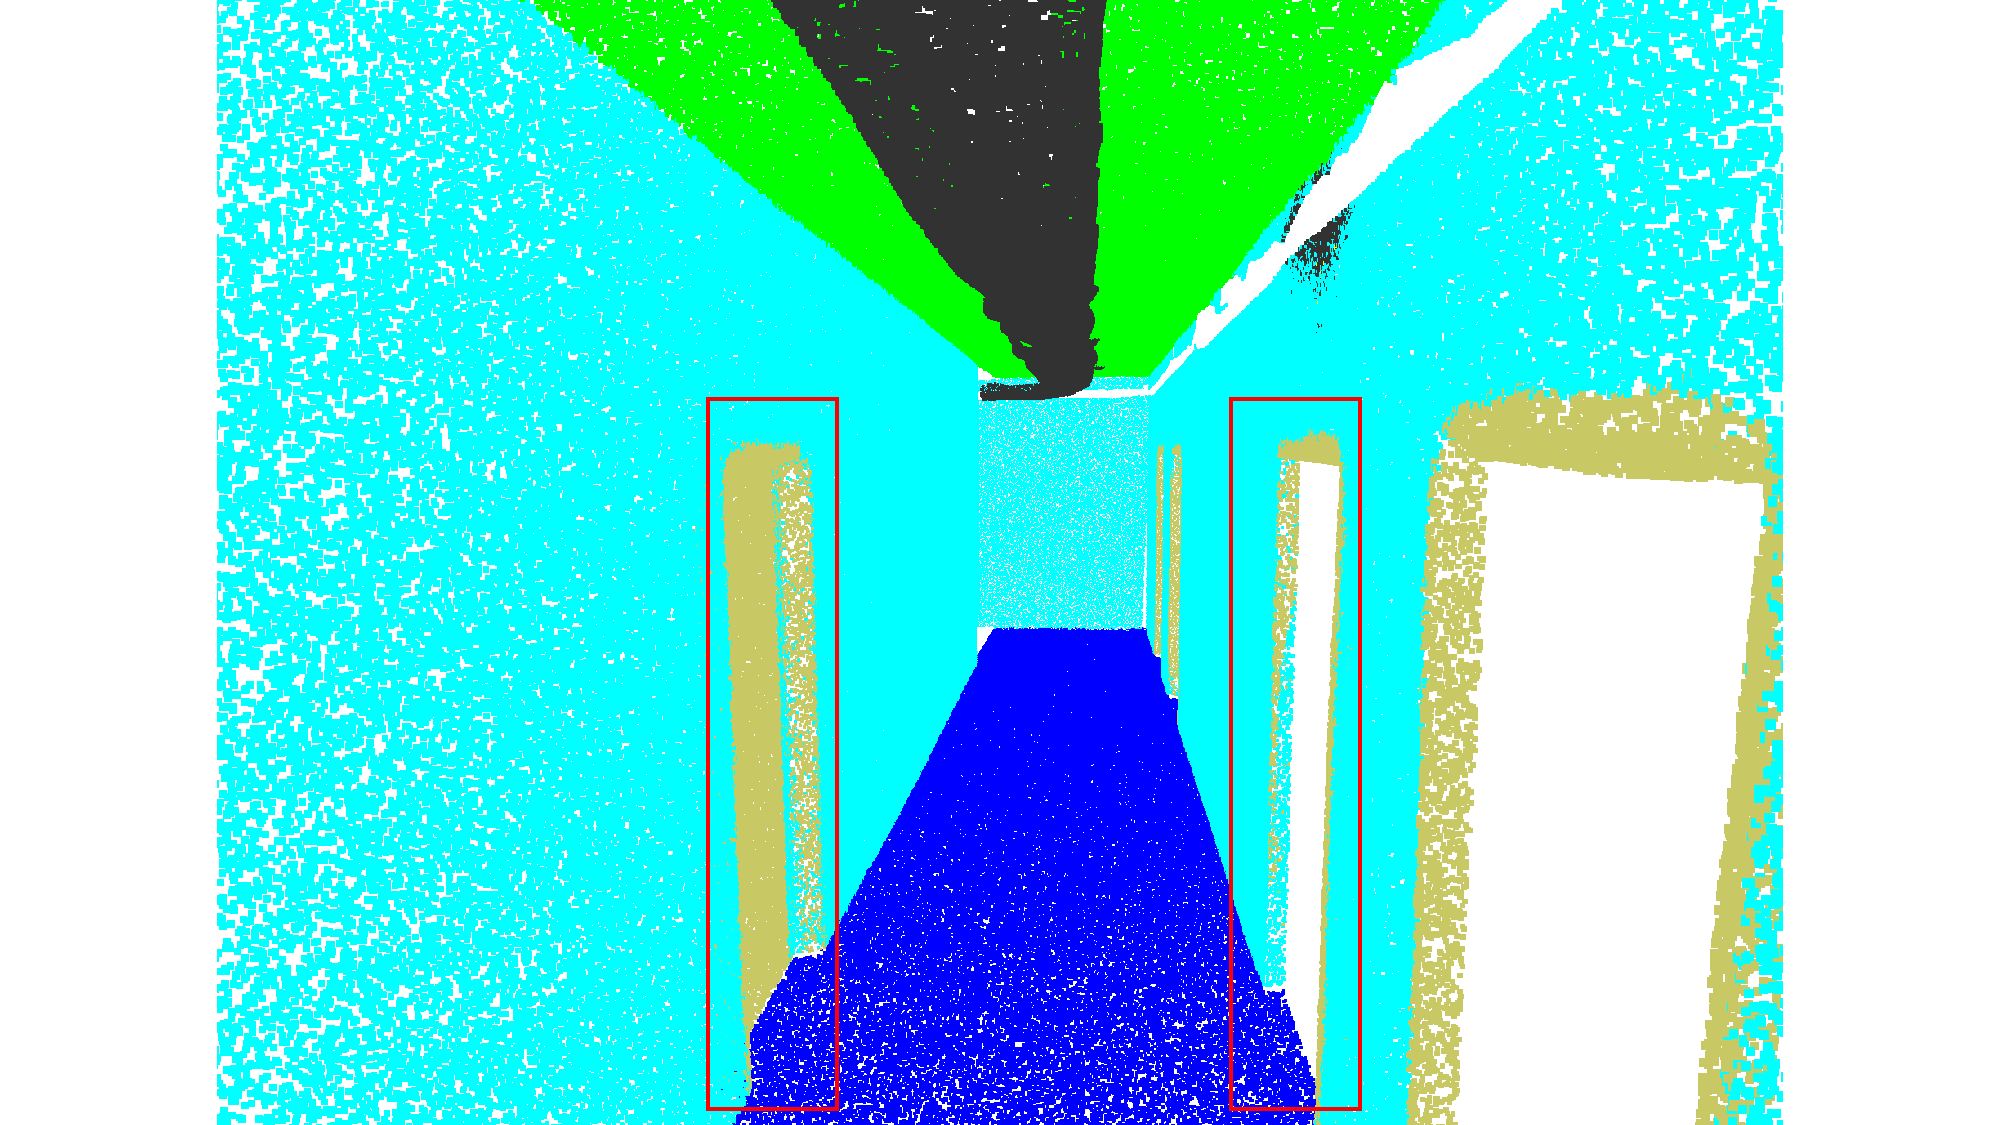
\includegraphics[width=\textwidth]{fig/supplement/semantic_segmentation/hallway_10/PLT_hallway_10.pdf}
    \end{minipage}
    \hfill
    \begin{minipage}{0.22\textwidth}
        \centering
        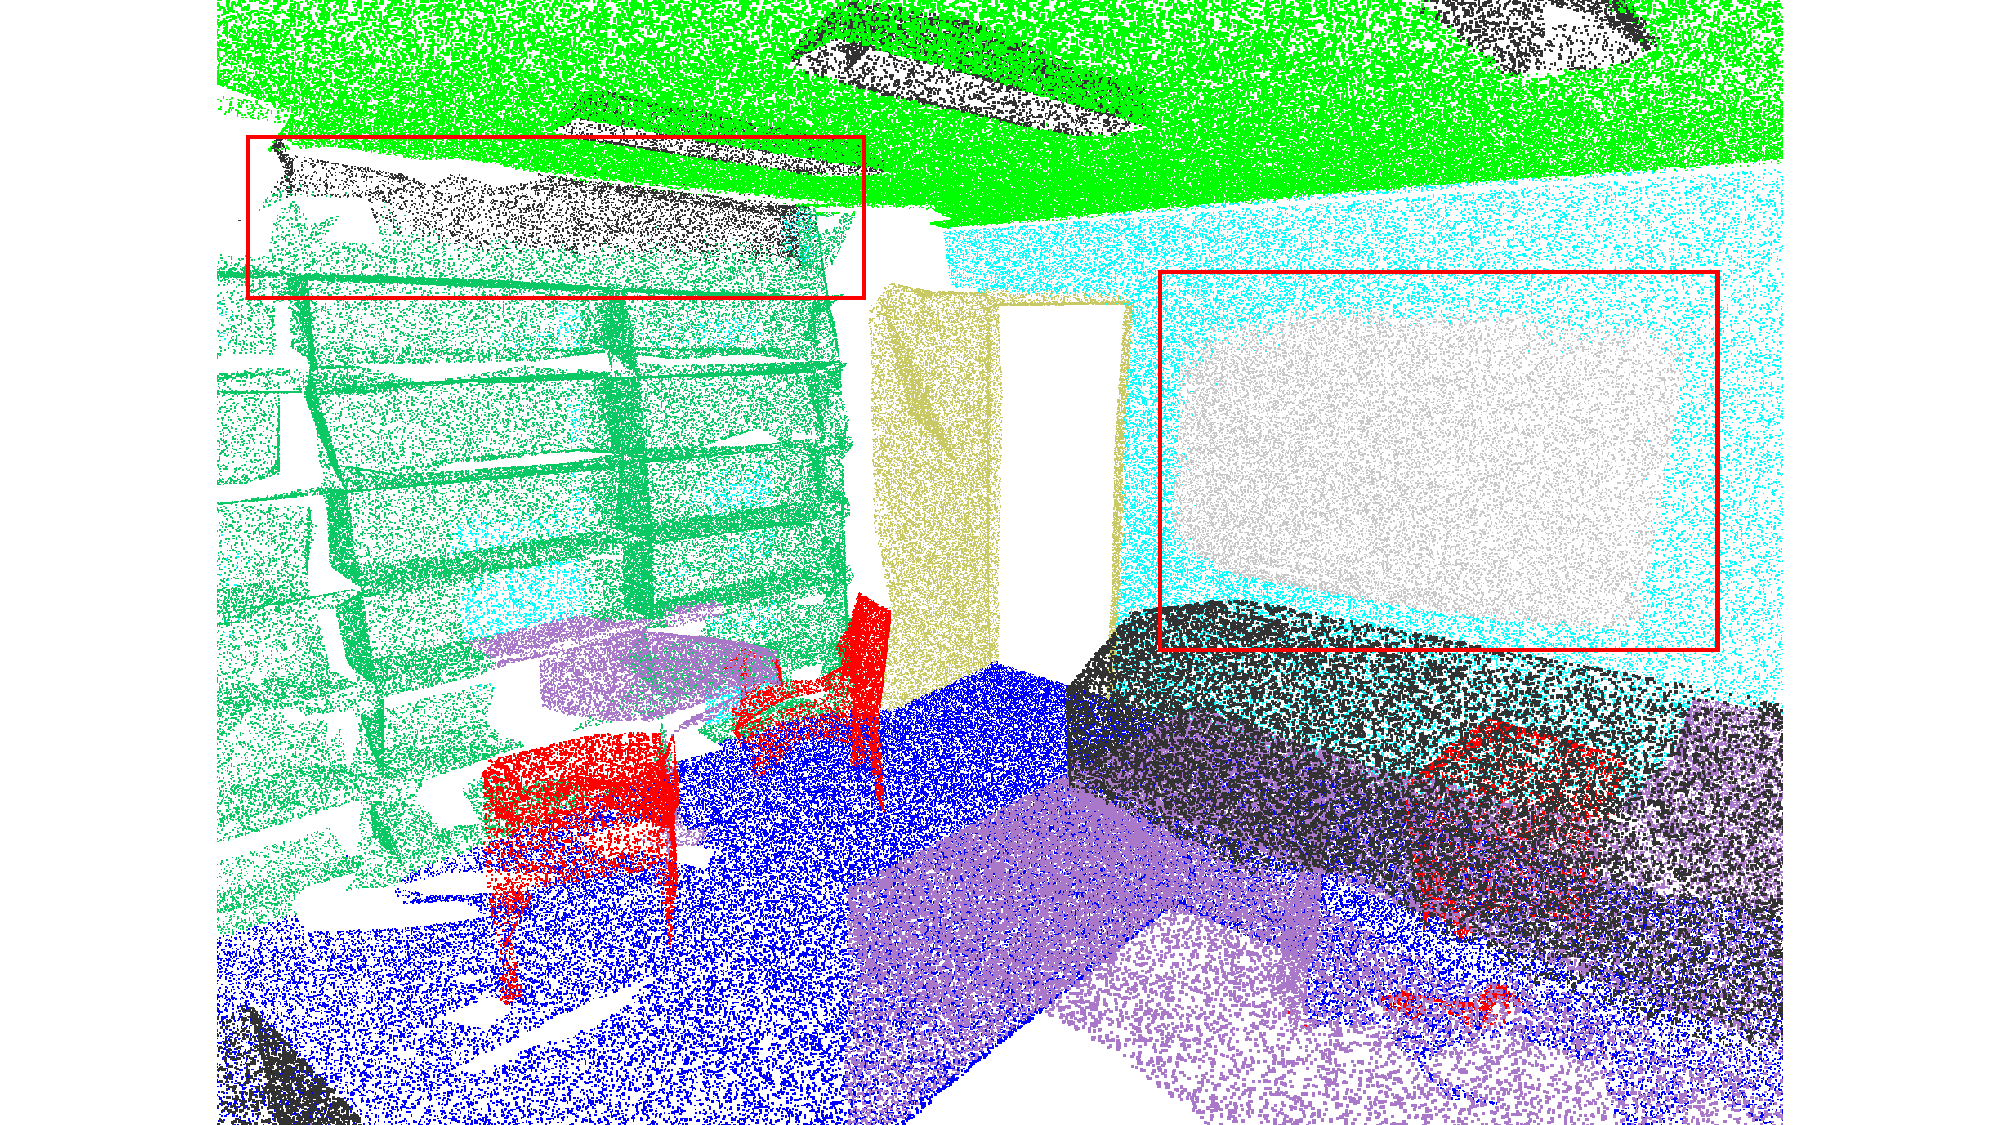
\includegraphics[width=\textwidth]{fig/supplement/semantic_segmentation/office_35/PLT_office_35.pdf}
    \end{minipage}
    \hfill
    \begin{minipage}{0.22\textwidth}
        \centering
        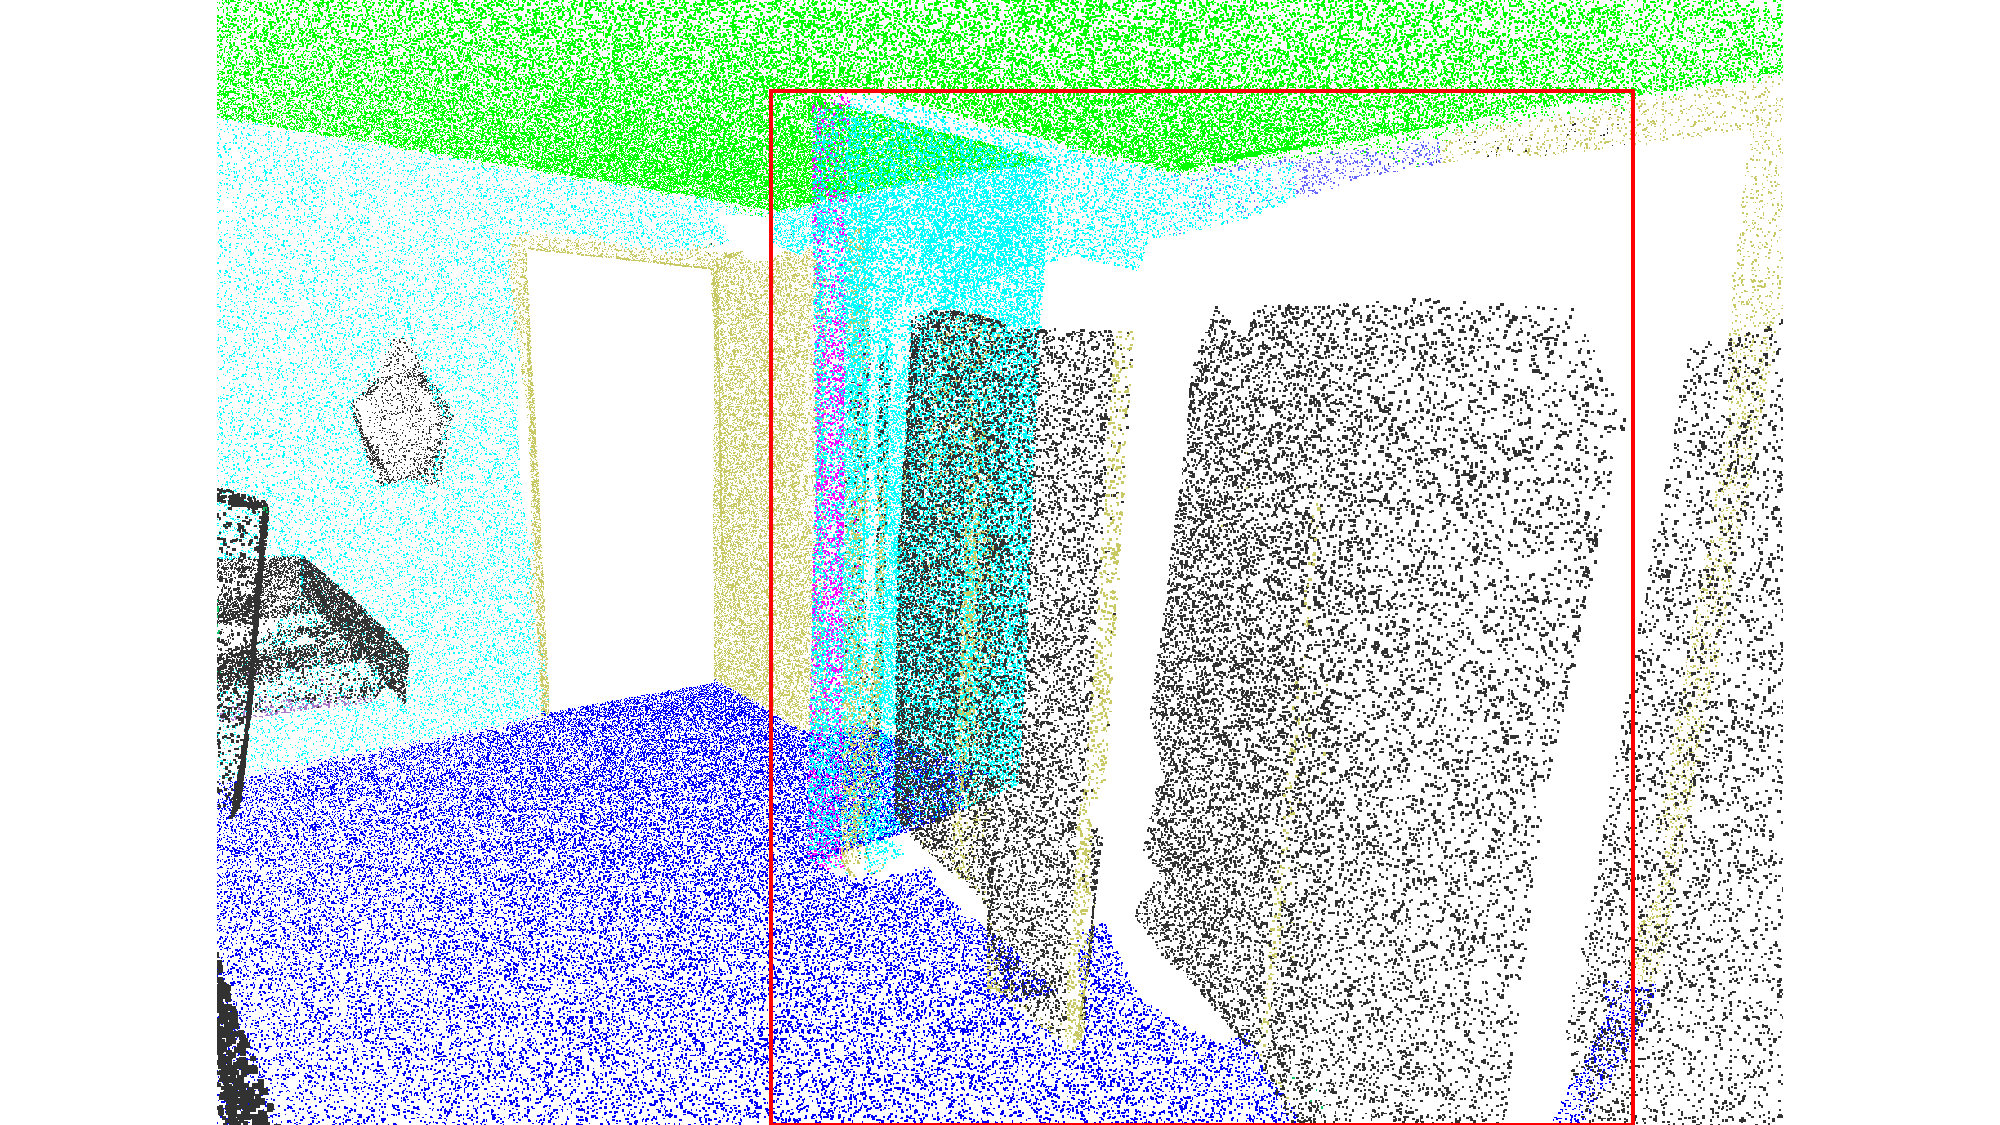
\includegraphics[width=\textwidth]{fig/supplement/semantic_segmentation/wc_2/PLT_wc_2.pdf}
    \end{minipage}
    \hfill

    % 换行
    \vspace{0.5em}

    % 第七行左侧的竖排标签
    \begin{minipage}{0.09\textwidth}
        \centering
        GT
    \end{minipage}
    \hfill
    % 第七行图片
    \begin{minipage}{0.22\textwidth}
        \centering
        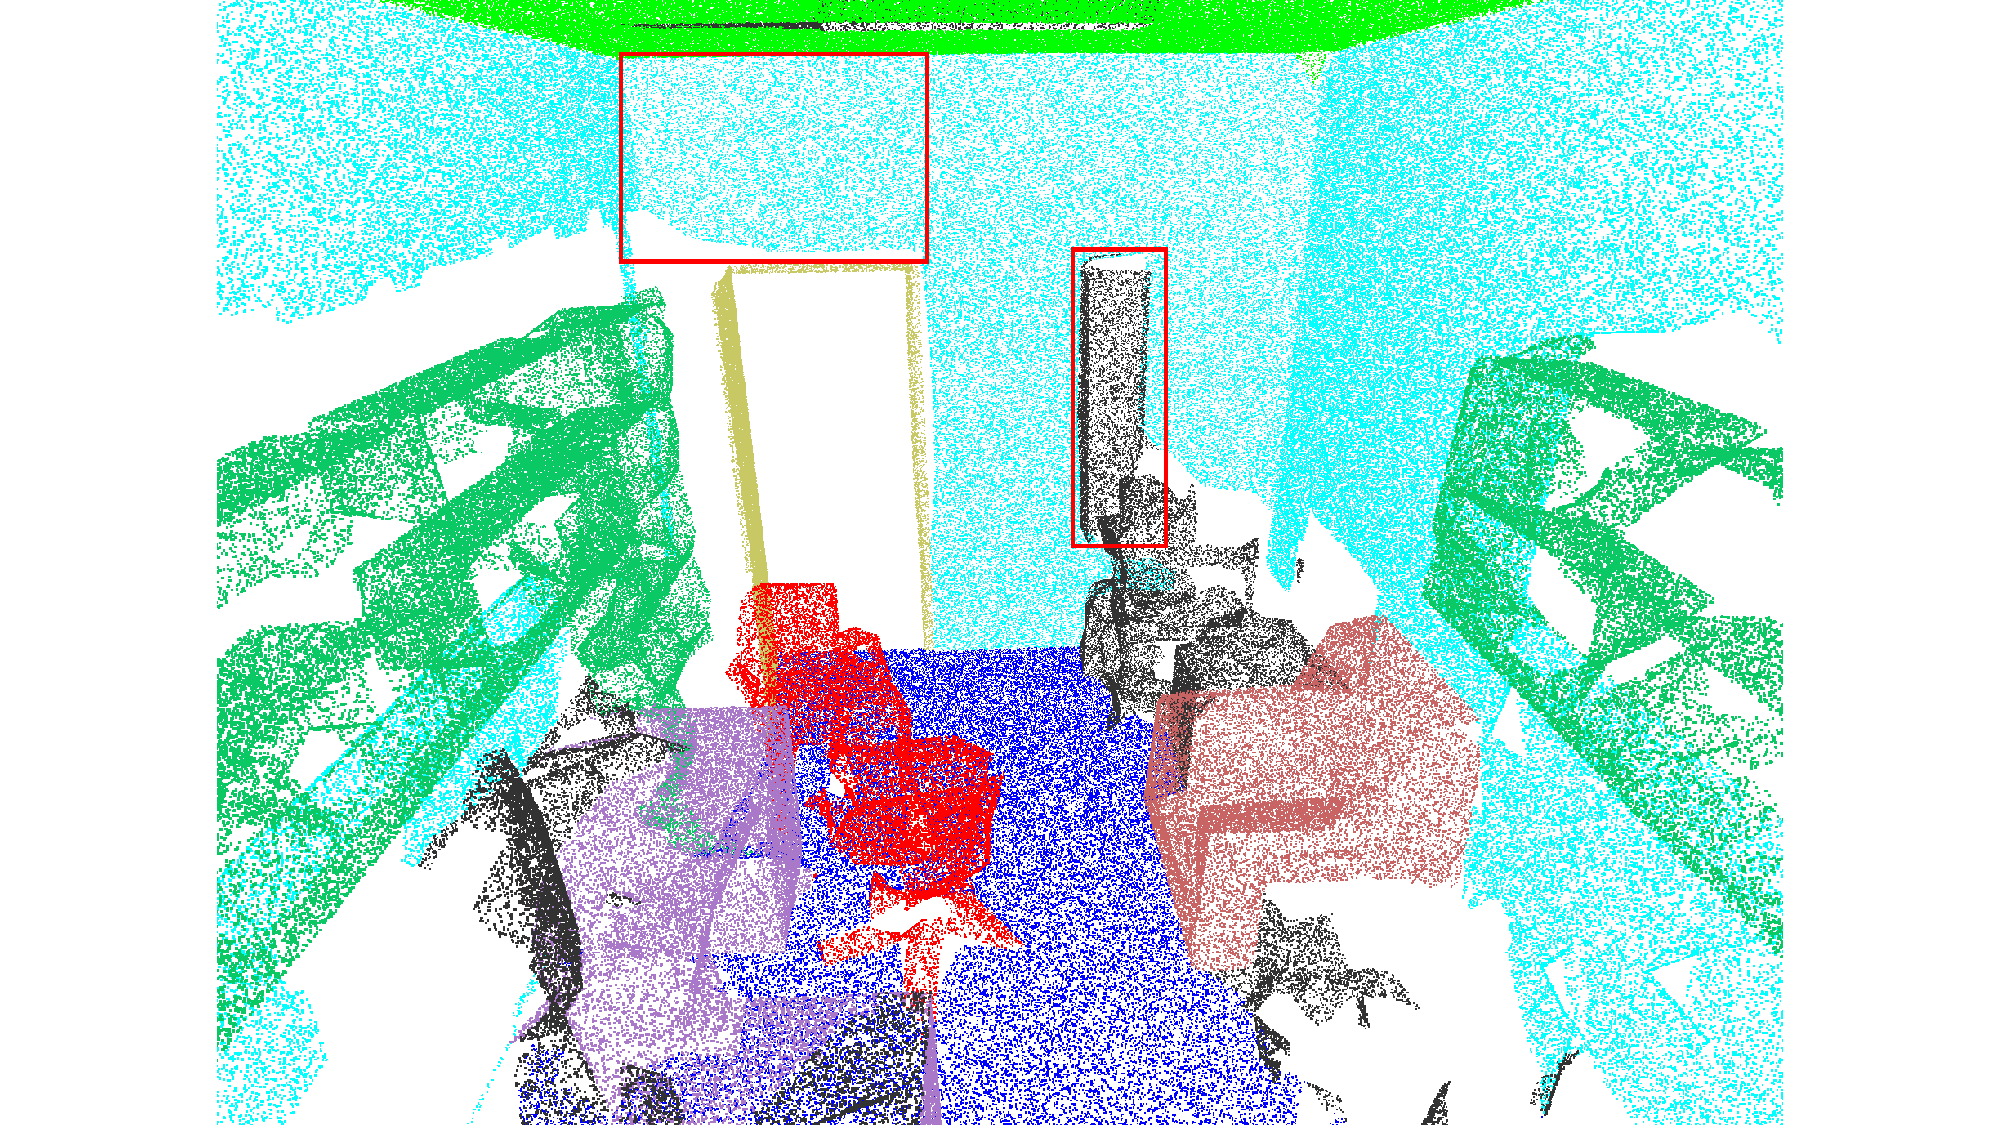
\includegraphics[width=\textwidth]{fig/supplement/semantic_segmentation/office_9/GT_office_9.pdf}
    \end{minipage}
    \hfill
    \begin{minipage}{0.22\textwidth}
        \centering
        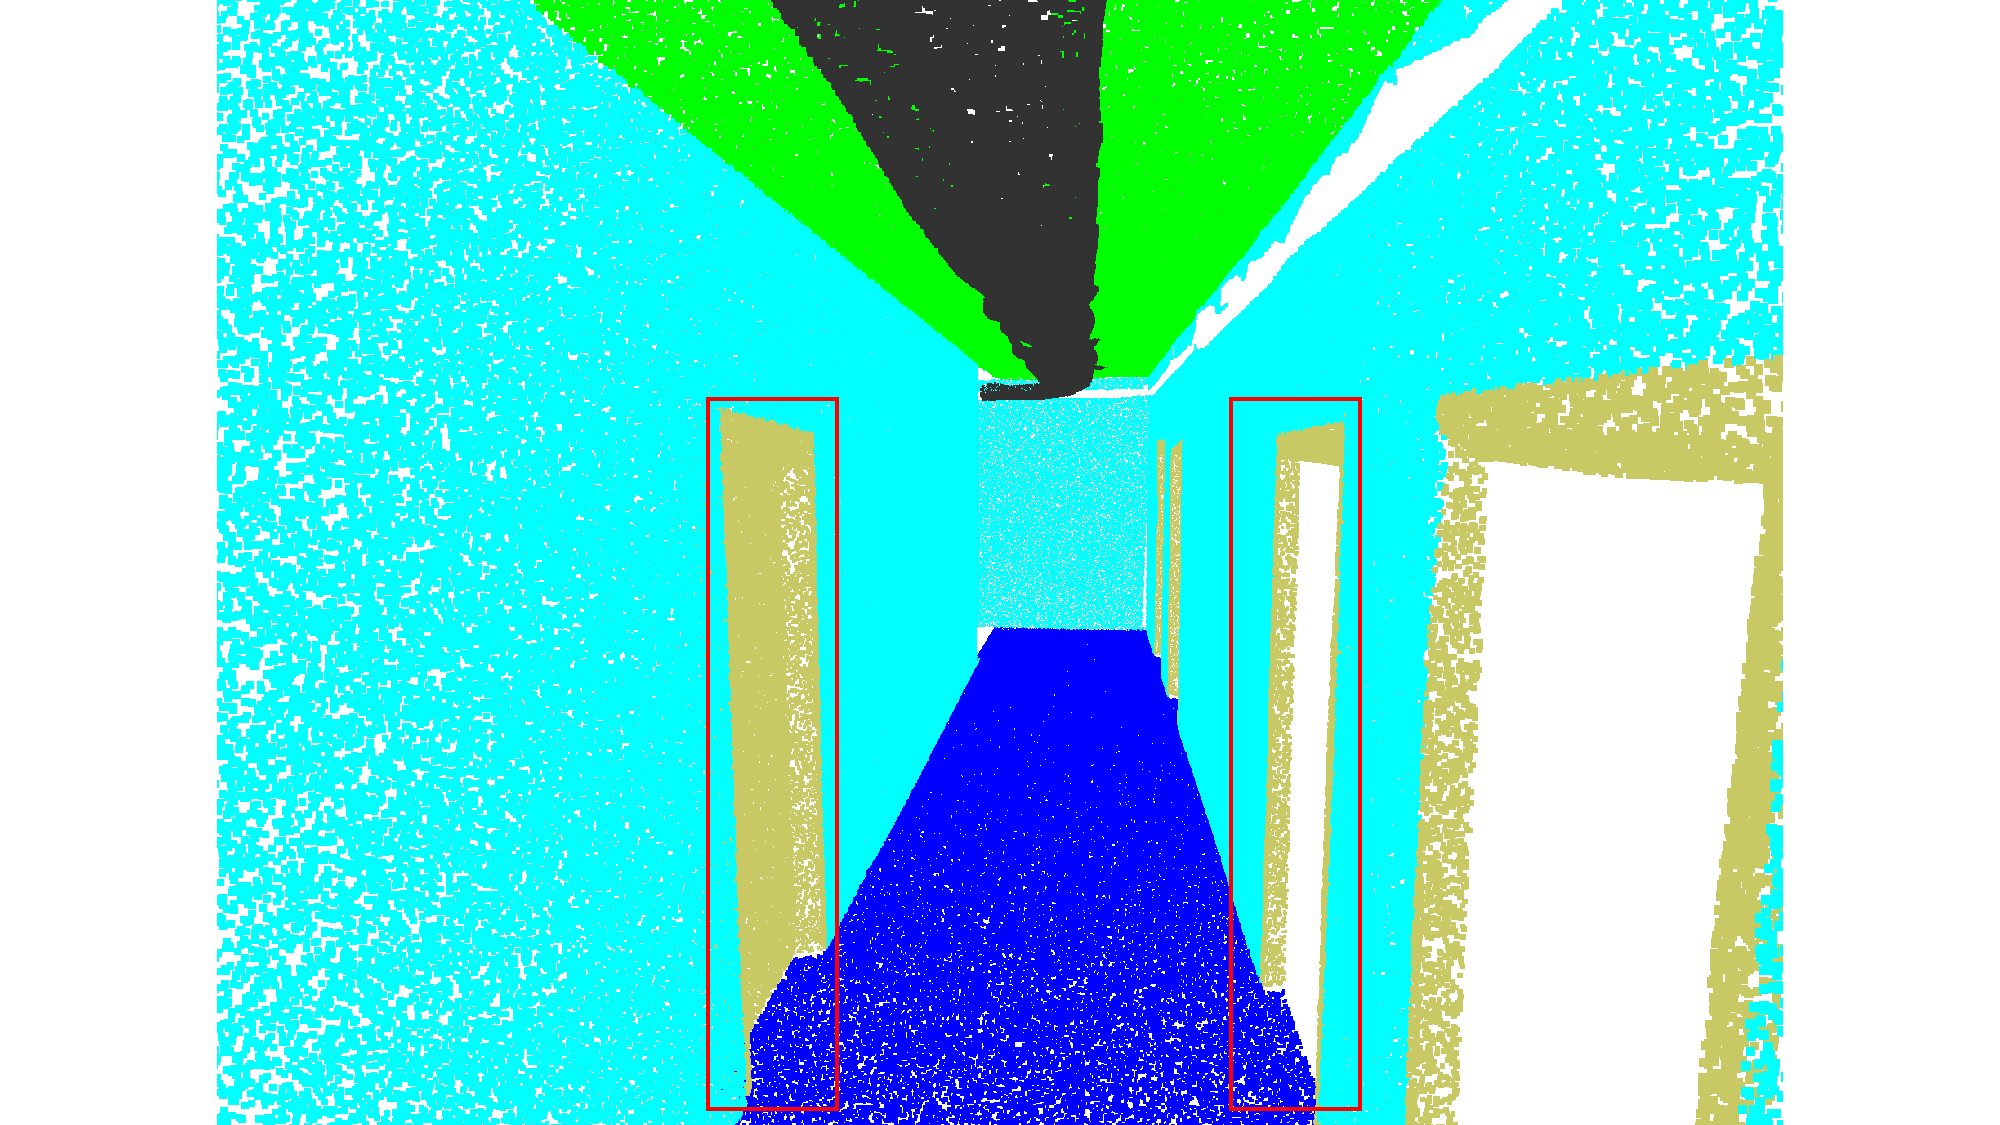
\includegraphics[width=\textwidth]{fig/supplement/semantic_segmentation/hallway_10/GT_hallway_10.pdf}
    \end{minipage}
    \hfill
    \begin{minipage}{0.22\textwidth}
        \centering
        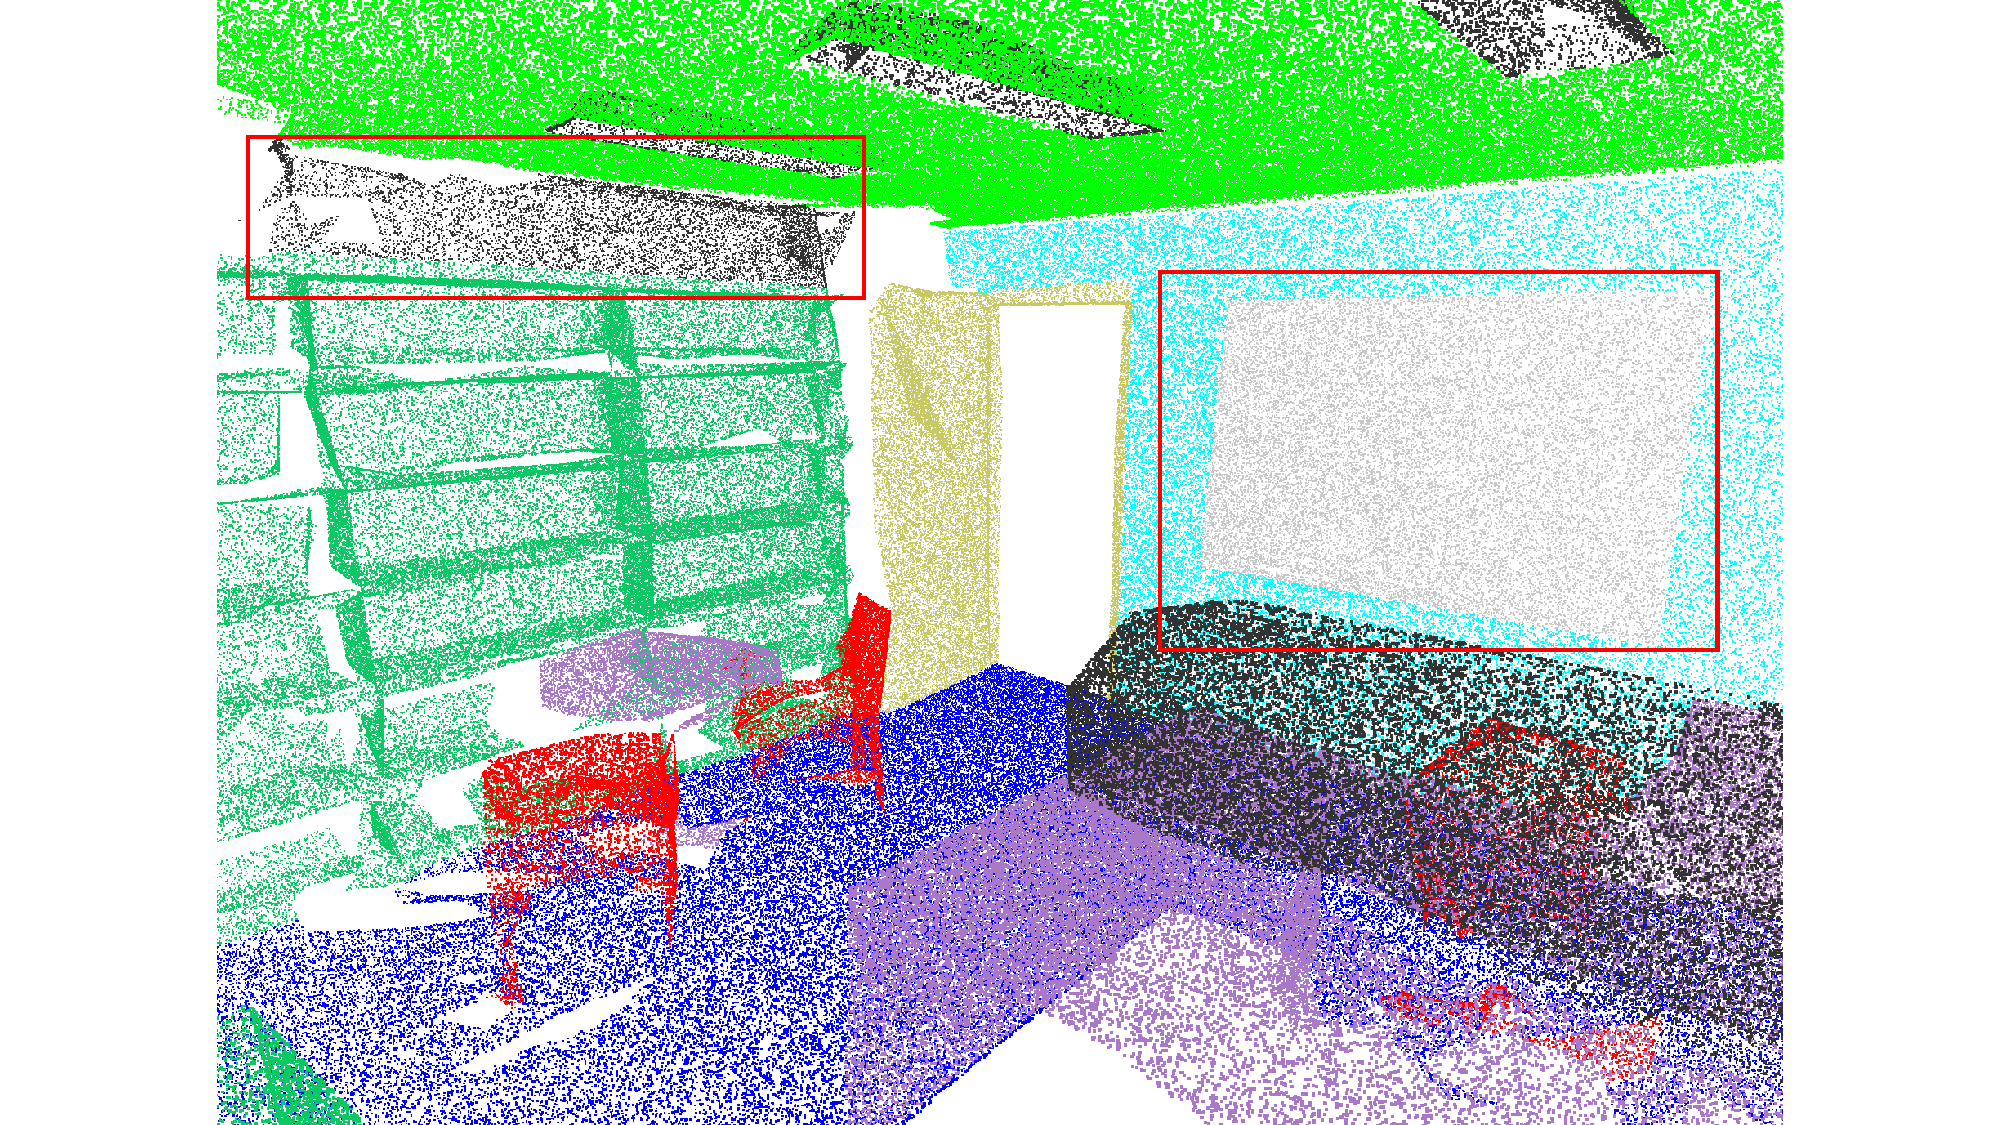
\includegraphics[width=\textwidth]{fig/supplement/semantic_segmentation/office_35/GT_office_35.pdf}
    \end{minipage}
    \hfill
    \begin{minipage}{0.22\textwidth}
        \centering
        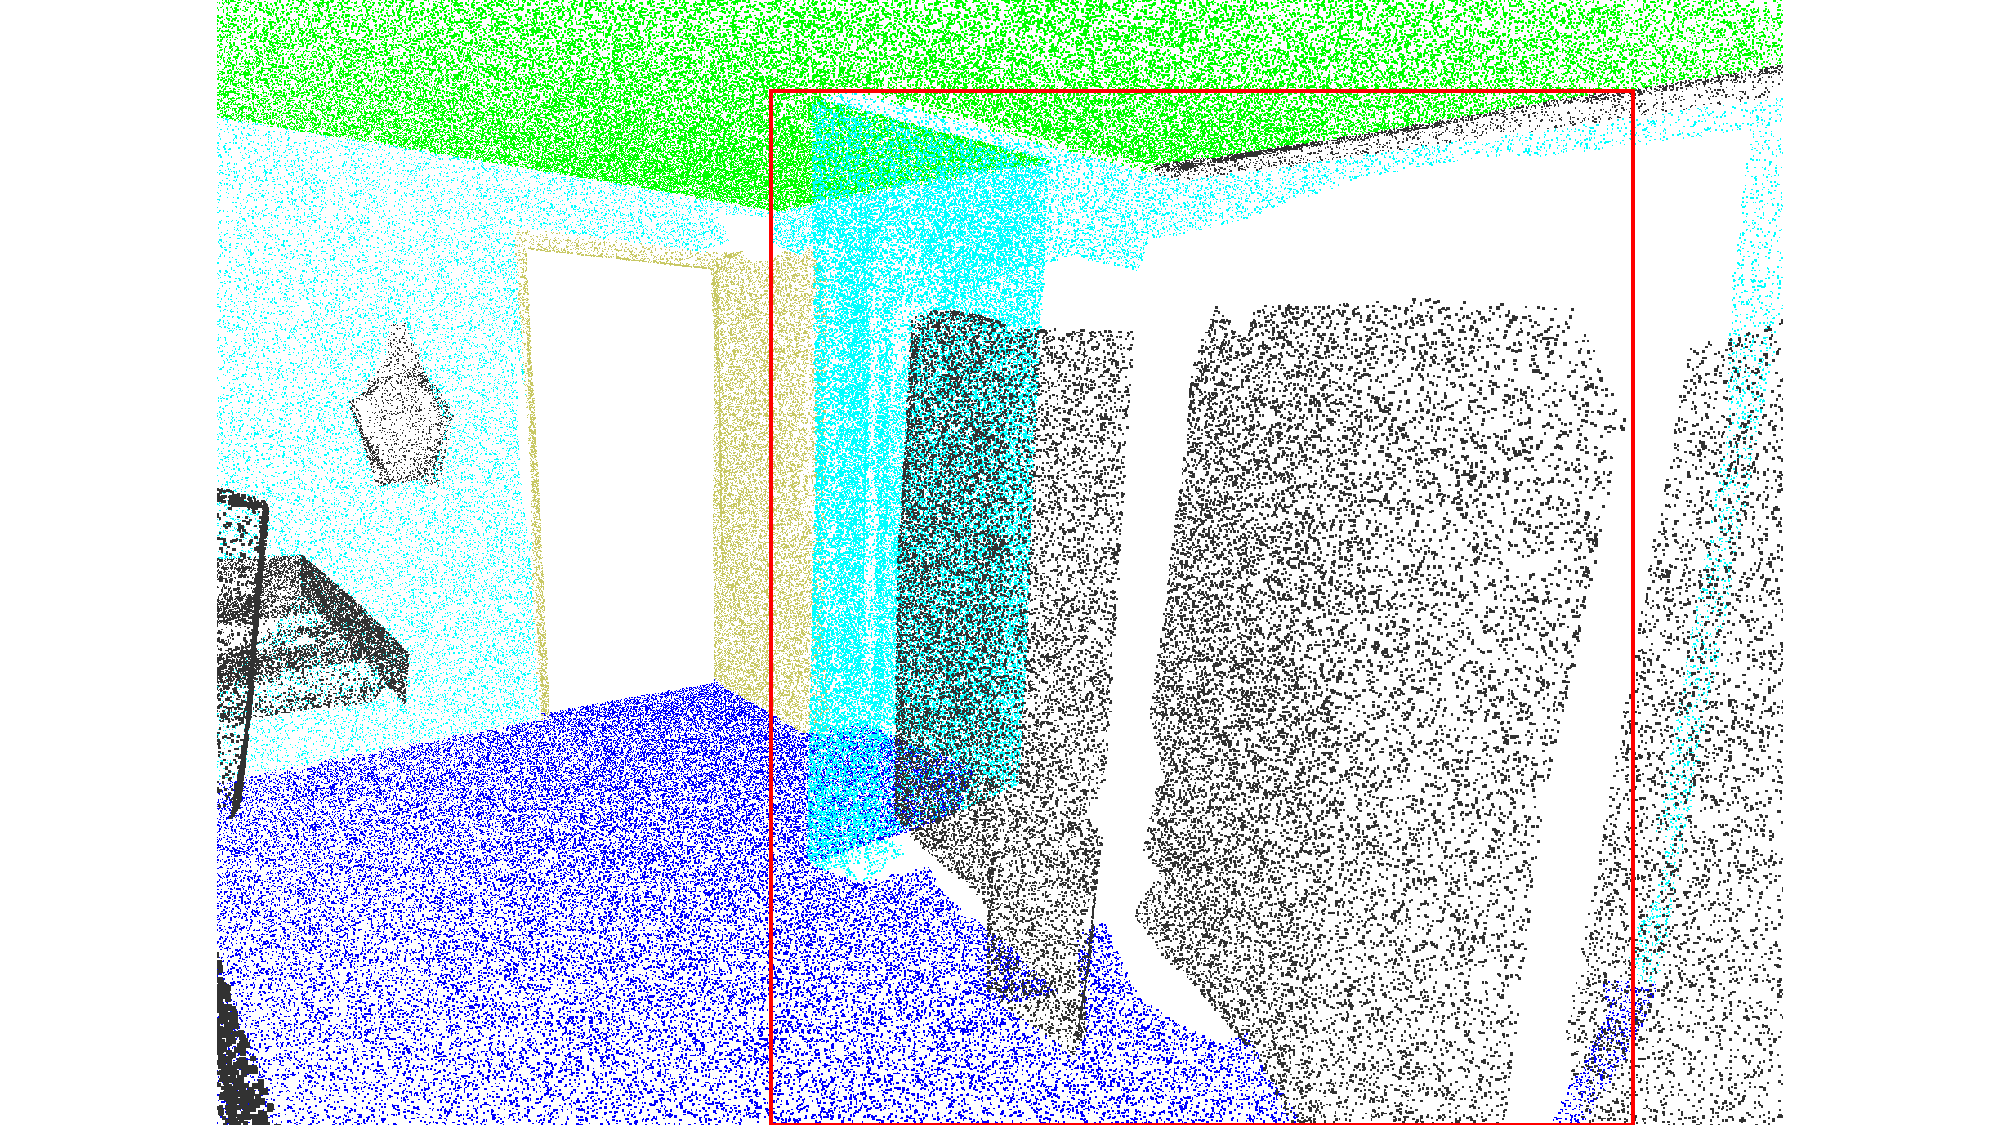
\includegraphics[width=\textwidth]{fig/supplement/semantic_segmentation/wc_2/GT_wc_2.pdf}
    \end{minipage}
    \hfill
    
    %下方的标签
    \vspace{0.5em}
    \begin{minipage}{0.09\textwidth} % 左侧空白区域
        \color{white}{12}
    \end{minipage}
    \hfill
    \begin{minipage}{0.22\textwidth} % 第2列标题
        \centering
        office\_9
    \end{minipage}
    \hfill
    \begin{minipage}{0.22\textwidth} % 第1列标题
        \centering
        hallway\_10
    \end{minipage}
    \hfill
    \begin{minipage}{0.22\textwidth} % 第3列标题
        \centering
        office\_35
    \end{minipage}
    \hfill
    \begin{minipage}{0.22\textwidth} % 第3列标题
        \centering
        wc\_2
    \end{minipage}
    \hfill
    \caption{The visualization of qualitative results for point cloud semantic segmentation. We compare our PLT with previous methods on Area 5 of the S3DIS dataset~\cite{armeni20163d}.}
    \label{fig:s3dis_1}

\end{figure*}


\begin{table}[!t]
\scriptsize
\setlength{\tabcolsep}{4.5mm}
\centering
 % \footnotesize
\caption{The effect of each component of our LST. SSF and DP represent Scale\&Shift Fine-tuning and Dynamic Prompt respectively. The tunable parameters (\#TP) and the overall accuracy (\%) on the hardest variant of ScanObjectNN\cite{uy2019revisiting} are reported.}
\label{tab:part}

\begin{tabular}{ ccccc }
   \toprule
 SSF & DP & HLN &  \#TP (M) & PB\_T50\_RS \\
\midrule
\multicolumn{3}{c}{Full fine-tuning}  &22.1 & 85.18 \\
\multicolumn{3}{c}{Linear Probing}  &0.27 & 75.99 \\
\midrule
&\ding {52} &\ding {52}& 0.49 & 84.52 \\
\ding {52}  & &\ding {52}& 0.60 &84.66 \\
\ding {52}  & & & 0.37 & 83.34\\
\rowcolor{linecolor!40}\ding {52}  &\ding {52} &\ding {52}  & 0.60 & \textbf{85.53} \\
\bottomrule
\end{tabular}
\end{table}

\begin{table}[!t]
\scriptsize
\setlength{\tabcolsep}{7.3mm}
\centering
\caption{Fusion way for local and global information in point clouds. The tunable parameters (\#TP) and the overall accuracy (\%) on the hardest variant of ScanObjectNN\cite{uy2019revisiting} are reported.}
\vspace{-10pt}
\label{tab:fusion_way}

\begin{tabular}{ccc}
\toprule
Fusion Way & \#TP (M) & PB\_T50\_RS \\
\midrule
Add & 0.58 & 85.01 \\
Concat & 0.62 & 84.63 \\
Only Global & 0.56 & 84.52 \\
Only Local & 0.56 & 82.86 \\
LGA with Sigmoid & 0.59 & 84.59 \\
\rowcolor{linecolor!40}LGA with Softmax & 0.60 & \textbf{85.46} \\
\bottomrule
\end{tabular}
% \vspace{-10pt}
\end{table}


\begin{table}[!t]
\scriptsize
\setlength{\tabcolsep}{7.8mm}
\centering
\caption{Comparison between HLN and PLT. The tunable parameters (\#TP) and the overall accuracy (\%) on the hardest variant of ScanObjectNN are reported. }
\vspace{-10pt}
\label{tab:sidenet}

\begin{tabular}{ccc}
\toprule
Method & \#TP (M) & PB\_T50\_RS \\
\midrule
Point-MAE & 22.1 & 85.18 \\
% Linear probing & 0.3 & 75.99 \\
HLN & 0.2 & 80.74 \\
\rowcolor{linecolor!40} PLT(Ours) & 0.6 & \textbf{85.46} \\
\bottomrule
\end{tabular}
% \vspace{-15pt}
\end{table}


\subsection{Ablation Study}

\textbf{Analysis of Each Component.} We conduct experiments to evaluate the effectiveness of the proposed components in PLT. As shown in Tab.~\ref{tab:part}, the performance on PB T50 RS reaches 85.46\% when all modules are included. However, removing any single module results in a performance decrease, emphasizing the importance of each component.

\textbf{Hyperparameter Ablation for Hierarchical Ladder Network.} We further explore the hyperparameters of the Hierarchical Ladder Network (HLN), as displayed in Tab.~\ref{tab:ablation}. Results indicate that optimal performance is achieved with 3 layers, feature dimensions of [16, 32, 64, 128], and neighbor counts of [16, 8, 4].

\textbf{Fusion Strategy for Local and Global Information.} In Tab.~\ref{tab:fusion_way}, we assess various fusion methods and observe that the proposed Local-Global Fusion (LGF) with Softmax yields the best results. Notably, using only local information performs worse than using only global information, possibly because local features are learned from scratch, whereas global features leverage pre-trained prior knowledge.

\textbf{Comparison Between HLN and PLT.} Tab.~\ref{tab:sidenet} shows that training with HLN alone leads to a substantial performance drop of 4.72\% compared to full fine-tuning, likely due to the lack of pre-trained global priors. However, integrating HLN with the backbone network through PLT results in higher performance than full fine-tuning.

%\subsection{Ablation Study}

%\textbf{Analysis on each component.}We conduct experiments to prove the effectiveness of the proposed components of Our PLT. As shown in the Tab.~\ref{tab:part}, when all modules are used, the performance on PB T50 RS reaches 85.46\%. However, removing any of the proposed modules leads to performance degradation, further highlighting the necessity of each module.

%\textbf{Ablation on hyper-parameters.} We conduct an in-depth exploration of the hyperparameters of Hierarchical Ladder Network (HLN), as shown in the Tab.~\ref{tab:ablation}, and found that the performance is optimal when the number of layers is 3, with feature dimensions of [16, 32, 64, 128], and the number of neighbors set to [16, 8, 4].

%\textbf{Fusion way for or local and global information in point clouds.} As shown in the Tab.~\ref{tab:fusion_way}, we explored various fusion methods and found that the proposed LGF with Softmax achieved the best performance. Additionally, when using only local information, the performance was worse than using only global information. This may be due to the fact that local information is learned from scratch, while global information benefits from pre-trained prior knowledge.

%\textbf{Comparison between HLN and PLT.} As shown in the Tab.~\ref{tab:sidenet}, when training with only HLN, we observed a significant performance drop of 4.72\% compared to full fine-tuning, likely due to the absence of pre-trained global prior information. However, by using our proposed PLT to integrate the features of both HLN and the backbone network, we achieved superior performance than full fine-tuning.

% \subsection{Visualization}